%%%%%%%%%%%%%%%%%%%%%%%%%%%%%%%%%%%%%%%%%
% Masters/Doctoral Thesis 
% LaTeX Template
% Version 1.43 (17/5/14)
%
% This template has been downloaded from:
% http://www.LaTeXTemplates.com
%
% Original authors:
% Steven Gunn 
% http://users.ecs.soton.ac.uk/srg/softwaretools/document/templates/
% and
% Sunil Patel
% http://www.sunilpatel.co.uk/thesis-template/
%
% License:
% CC BY-NC-SA 3.0 (http://creativecommons.org/licenses/by-nc-sa/3.0/)
%
% Note:
% Make sure to edit document variables in the Thesis.cls file
%
%%%%%%%%%%%%%%%%%%%%%%%%%%%%%%%%%%%%%%%%%

%----------------------------------------------------------------------------------------
%	PACKAGES AND OTHER DOCUMENT CONFIGURATIONS
%----------------------------------------------------------------------------------------

\documentclass[11pt, oneside]{Thesis} % The default font size and one-sided printing (no margin offsets)

\graphicspath{{Pictures/}} % Specifies the directory where pictures are stored

\usepackage{comment}
\usepackage[square, numbers, comma, sort&compress]{natbib} % Use the natbib reference package - read up on this to edit the reference style; if you want text (e.g. Smith et al., 2012) for the in-text references (instead of numbers), remove 'numbers' 
\hypersetup{urlcolor=blue, colorlinks=true} % Colors hyperlinks in blue - change to black if annoying
\title{\ttitle} % Defines the thesis title - don't touch this

\begin{document}

\frontmatter % Use roman page numbering style (i, ii, iii, iv...) for the pre-content pages

\setstretch{1.3} % Line spacing of 1.3

% Define the page headers using the FancyHdr package and set up for one-sided printing
\fancyhead{} % Clears all page headers and footers
\rhead{\thepage} % Sets the right side header to show the page number
\lhead{} % Clears the left side page header

\pagestyle{fancy} % Finally, use the "fancy" page style to implement the FancyHdr headers

\newcommand{\HRule}{\rule{\linewidth}{0.5mm}} % New command to make the lines in the title page

% PDF meta-data
\hypersetup{pdftitle={\ttitle}}
\hypersetup{pdfsubject=\subjectname}
\hypersetup{pdfauthor=\authornames}
\hypersetup{pdfkeywords=\keywordnames}

%----------------------------------------------------------------------------------------
%	TITLE PAGE
%----------------------------------------------------------------------------------------

\begin{titlepage}
\begin{center}
\textsc{\LARGE \univname}\\[1.5cm] % University name
\textsc{\Large Master Thesis}\\[0.5cm] % Thesis type

\HRule \\[0.4cm] % Horizontal line
{\huge \bfseries \ttitle}\\[0.4cm] % Thesis title
\HRule \\[1.5cm] % Horizontal line
 
\begin{minipage}{0.4\textwidth}
\begin{flushleft} \large
\emph{Author:}\\
\href{http://www.johnsmith.com}{\authornames} % Author name - remove the \href bracket to remove the link
\end{flushleft}
\end{minipage}
\begin{minipage}{0.4\textwidth}
\begin{flushright} \large
\emph{Supervisor:} \\
\href{http://soa.cmu.edu/nina-baird/}{\supname} % Supervisor name - remove the \href bracket to remove the link  
\end{flushright}
\end{minipage}\\[3cm]
 
\large \textit{A thesis submitted in fulfilment of the requirements\\ for the degree of \degreename}\\[0.3cm] % University requirement text
\textit{in the}\\[0.4cm]
\groupname\\\deptname\\[2cm] % Research group name and department name
 
{\large \today}\\[4cm] % Date
%\includegraphics{Logo} % University/department logo - uncomment to place it
 
\vfill
\end{center}

\end{titlepage}

%----------------------------------------------------------------------------------------
%	DECLARATION PAGE
%	Your institution may give you a different text to place here
%----------------------------------------------------------------------------------------

\Declaration{

\addtocontents{toc}{\vspace{1em}} % Add a gap in the Contents, for aesthetics

I, \authornames, declare that this thesis titled, '\ttitle' and the work presented in it are my own. I confirm that:

\begin{itemize} 
\item[\tiny{$\blacksquare$}] This work was done wholly or mainly while in candidature for a research degree at this University.
\item[\tiny{$\blacksquare$}] Where any part of this thesis has previously been submitted for a degree or any other qualification at this University or any other institution, this has been clearly stated.
\item[\tiny{$\blacksquare$}] Where I have consulted the published work of others, this is always clearly attributed.
\item[\tiny{$\blacksquare$}] Where I have quoted from the work of others, the source is always given. With the exception of such quotations, this thesis is entirely my own work.
\item[\tiny{$\blacksquare$}] I have acknowledged all main sources of help.
\item[\tiny{$\blacksquare$}] Where the thesis is based on work done by myself jointly with others, I have made clear exactly what was done by others and what I have contributed myself.\\
\end{itemize}
 
Signed:\\
\rule[1em]{25em}{0.5pt} % This prints a line for the signature
 
Date:\\
\rule[1em]{25em}{0.5pt} % This prints a line to write the date
}

\clearpage % Start a new page

\begin{comment}
%----------------------------------------------------------------------------------------
%	QUOTATION PAGE
%----------------------------------------------------------------------------------------

\pagestyle{empty} % No headers or footers for the following pages

\null\vfill % Add some space to move the quote down the page a bit

\textit{``My passion and great enjoyment for architecture, and the reason the older I get the more I enjoy it, is because I believe we - architects - can effect the quality of life of the people."}

\begin{flushright}
Richard Rogers
\end{flushright}

\vfill\vfill\vfill\vfill\vfill\vfill\null % Add some space at the bottom to position the quote just right

\clearpage % Start a new page
\end{comment}

%----------------------------------------------------------------------------------------
%	ABSTRACT PAGE
%----------------------------------------------------------------------------------------

\addtotoc{Abstract} % Add the "Abstract" page entry to the Contents

\abstract{\addtocontents{toc}{\vspace{1em}} % Add a gap in the Contents, for aesthetics

  The project aims at implementing a Dynamic Energy Demand Map that
  holds, visualizes and analyzes high spatial (each building, building
  group and the community) temporal (hourly) resolution energy demand
  data of a community with the focus on creating a highly integrated
  visualization and an interface is designed to serve this
  purpose. The target user of the interface is researchers in energy
  related fields with the basic abilities of map reading,
  understanding moderately complicated map legend and data plot and
  understanding building energy performance attributes and their
  implications. A general purpose design is created to provide both
  qualitative and quantitative information and to suit different
  research interest of this user group.

  The approach is demonstrated with a conceptual community model
  created in CityEngine based on the land use pattern of a mixed-use
  redevelopment project at Lower Hill District, Pittsburgh, PA. The
  hourly energy demand profile is retrieved from the simulation of DOE
  Commercial Prototype Building ASHRAE90.1-2013.
  
\clearpage % Start a new page

\begin{comment}
%----------------------------------------------------------------------------------------
%	ACKNOWLEDGEMENTS
%----------------------------------------------------------------------------------------

\setstretch{1.3} % Reset the line-spacing to 1.3 for body text (if it has changed)

\acknowledgements{\addtocontents{toc}{\vspace{1em}} % Add a gap in the Contents, for aesthetics

\par I would like to thank my advisor Prof. Volker Hartkopf for the guidance and help in establishing many connections.
\par I would like to thank Ms. Anne-Marie Lubenau for the kindly
sharing of her previous design of a Senior Community Center in the
proposed site.
\par I would like to thank Dr. Sharon Carver and Miss Allison Drash
from the children's school of Carnegie Mellon University who provided
valuable insights on the project.
\par I would like to thank Ms. Lyn Decker from Osher Lifelong Learning
Institute for her kindly help in helpping me understand more about the
life of the elderly and the potential opportunities and challenges.
\par I would like to thank Prof. Kristen Kurland for her comments and
ideas about the project and a list of valuable connections.
\par I would also like to thank Prof. Sean Qian for his guidance of me
through the GIS tools and the analysis method.  }
\clearpage % Start a new page

\end{comment}
%----------------------------------------------------------------------------------------
%	LIST OF CONTENTS/FIGURES/TABLES PAGES
%----------------------------------------------------------------------------------------

\pagestyle{fancy} % The page style headers have been "empty" all this time, now use the "fancy" headers as defined before to bring them back

\lhead{\emph{Contents}} % Set the left side page header to "Contents"
\tableofcontents % Write out the Table of Contents

\lhead{\emph{List of Figures}} % Set the left side page header to "List of Figures"
\listoffigures % Write out the List of Figures

\lhead{\emph{List of Tables}} % Set the left side page header to "List of Tables"
\listoftables % Write out the List of Tables

%----------------------------------------------------------------------------------------
%	ABBREVIATIONS
%----------------------------------------------------------------------------------------

\clearpage % Start a new page

\setstretch{1.5} % Set the line spacing to 1.5, this makes the following tables easier to read

\lhead{\emph{Abbreviations}} % Set the left side page header to "Abbreviations"
\listofsymbols{ll} % Include a list of Abbreviations (a table of two columns)
{
  \textbf{CMU} & \textbf{C}arnegie \textbf{M}ellon \textbf{U}niversity \\
  \textbf{GHG} & \textbf{G}reen\textbf{H}ouse\textbf{G}as\\
  \textbf{DOE} & the U.S. \textbf{D}epartment \textbf{O}f\textbf{E}nergy\\
  \textbf{HTPR} & \textbf{H}eat\textbf{T}o\textbf{P}ower \textbf{R}atio\\
  \textbf{EPM} & \textbf{E}nergy\textbf{P}otential\textbf{M}apping\\
  \textbf{EMIOFN} &\textbf{E}nergy \textbf{M}apping to \textbf{I}dentify \textbf{O}pportunities for \textbf{F}uture\\
%\textbf{Acronym} & \textbf{W}hat (it) \textbf{S}tands \textbf{F}or \\
}

\begin{comment}
%----------------------------------------------------------------------------------------
%	PHYSICAL CONSTANTS/OTHER DEFINITIONS
%----------------------------------------------------------------------------------------
\clearpage % Start a new page

\lhead{\emph{Physical Constants}} % Set the left side page header to "Physical Constants"

\listofconstants{lrcl} % Include a list of Physical Constants (a four column table)
{
Speed of Light & $c$ & $=$ & $2.997\ 924\ 58\times10^{8}\ \mbox{ms}^{-\mbox{s}}$ (exact)\\
% Constant Name & Symbol & = & Constant Value (with units) \\
}
\end{comment}

%----------------------------------------------------------------------------------------
%	SYMBOLS
%----------------------------------------------------------------------------------------


\clearpage % Start a new page
\lhead{\emph{Symbols}} % Set the left side page header to "Symbols"

\listofnomenclature{lll} % Include a list of Symbols (a three column table)
{
$THR$ & condenser total heat of rejection & Btuh \\
$RE $ & net refrigeration effect & Btuh \\
$f  $ & Heat Rejection Factor & 1 \\
% Symbol & Name & Unit \\

& & \\ % Gap to separate the Roman symbols from the Greek

% Symbol & Name & Unit \\
}
\begin{comment}
%----------------------------------------------------------------------------------------
%	DEDICATION
%----------------------------------------------------------------------------------------

\setstretch{1.3} % Return the line spacing back to 1.3

\pagestyle{empty} % Page style needs to be empty for this page

\dedicatory{Dedicated to my family, friends and my instructors\ldots} % Dedication text

\addtocontents{toc}{\vspace{2em}} % Add a gap in the Contents, for aesthetics

\end{comment}
%----------------------------------------------------------------------------------------
%	THESIS CONTENT - CHAPTERS
%----------------------------------------------------------------------------------------

\mainmatter % Begin numeric (1,2,3...) page numbering

\pagestyle{fancy} % Return the page headers back to the "fancy" style

% Include the chapters of the thesis as separate files from the Chapters folder
% Uncomment the lines as you write the chapters

% Chapter 1

\chapter{General Introduction} % Main chapter title

\label{Chapter1} % For referencing the chapter elsewhere, use \ref{Chapter1}

\lhead{Chapter 1. \emph{General Introduction}} % This is for the header on each page - perhaps a shortened title

%----------------------------------------------------------------------------------------

\section{Project Overview}
The burning of fossil fuels produces green house gases (GHG) and
causes significant global climate changes including global sea level
rise, temperature rise, ocean warming, ice sheet melting and extreme
weather events~\cite{NASA2015}. Fossil fuels are finite: studies have
shown that if the consumtion rate of fossil fuels remain the same, the
major fossil fuels including oil, gas and coal will run out by the end
of this century~\cite{Ecotricity2015, Kathryn2015}. Governments have
begun to make reducing GHG as one of their major development goals: UK
launched the ``Climate Change Act'' that aims at reducing GHG
emissions by 80\% comparing to 1990 by 2050~\cite{carbonBudgetUK}; the
City of Calgary aims at reducing CO$_2$ emission rate by 50\% by
2050~\cite{aacip2009}. In the U.S., the Climate Action Plan was
lauched by President Obama in Jun. 2013. The plan has set the GHG
reduction goal to 26 to 28\% by 2025 comparing with the 2005 level of
emissions~\cite{ghgReduce2014}.

Reducing GHG emissions and fossil fuel consumption also takes place at
the community level. Community Energy Management (CEM) is a
combination of community level design strategies and energy management
strategies aiming at providing quality of life in an urban environment
with minimized energy consumption and environmental
impact~\cite{Jaccard19971065}. It contains ``land use planning'',
``transportation management'', ``site planning'' and ``local energy
supply and delivery planning''~\cite{Jaccard19971065}. Community level
energy planning and management achieves GHG reduction by means of :1)
improving energy efficiency, 2) limiting the use of high quality
energy and 3) using renewable energy source ~\cite{StDenis20092088}.

Energy Mapping makes community energy planning alternatives visible to
planners and policy makers~\cite{baird2014} and thus becomes
increasingly popular with the increasing attention to community energy
planing. Emerging explorations of the role and power of Energy Mapping
in assisting community energy planning are taking place all over the
world. The City of Calgary carried out an Energy Mapping Study that
aims to ``encourage the use of alternative energy systems, through
considerations such as the design of buildings and encouragement of
more compact, mixed-use and high density
communities.''~\cite{baird2014}. The ``London Heat Map'' project helps
developers and planners to ``identify opportunities for decentralized
energy projects''~\cite{londonHeatMap}.

Energy mapping is still a developing field with variations in the
information included and its display. The Calgary Energy Mapping study
depicts annual average energy use intensity and alternative renewable
energy supply regions~\cite{aacip2009}. The London Heat Map contains
mainly heating energy related features: high heating energy consumers,
suppliers and district heating networks. The Dutch Heat Map, an
application of the Energy Potential Mapping (EPM) method developed by
Dobbelsteen et al.\ ~\cite{Dobbelsteen2013}, contains information of
annual heating energy demand (or demand density), heating energy
supply (or supply density), the infrastructure network layout and CHP
and biomass plant locations.

However, as suggested by Baird et al.\ , existing Energy Mapping
practices are mainly static, i.e. the time-dependent changes of energy
demand and supply information is not included in these Energy Maps nor
do they support more advanced community energy system analysis and
comparison. Thus the concept of ``Dynamic Energy
Mapping''~\cite{baird2014} was brought about. A dynamic energy map can:
\begin{enumerate}[i.]
\item Act as a geo-database that efficiently holds
  \begin{itemize}
  \item hourly energy profile data for each building and the
    aggregated energy profile data for the whole
    community~\cite{baird2014};
  \item hourly energy supply data of community~\cite{baird2014}.
  \end{itemize}
\item Visually display the dynamic energy demand and supply changes
  with high spatial and temporal resoltion~\cite{baird2014}.
\item Allow data analysis and support district system
  sizing~\cite{baird2014}.
\item Be connected to simulation tools that can support instant
  performance analysis~\cite{baird2014}.
\end{enumerate}
 
With a Dynamic Energy Map, the temporal behavior of the demand and
supply of heating, cooling and electricity can be revealed and
compared, analyzed and updated. One can see how well the supply meets
the demand over time. One can also use it as a key component of
Geo-design that encompasses ``geo-spatial modeling, impact
simulations, and real-time feedback to facilitate holistic designs and
smart decisions''~\cite{esriGeodesign2012}. The development of
data-driven approaches and machine learning methods could also be
coupled with the Energy Map to allow more complicated analysis of the
spatial-temporal behavior of energy data and provide more informative
design or management support.

\section{Objective and Problem Definition}
An initial instance of Dynamic Energy Map was created by Johnstone and
Baird and described in ~\cite{baird2014}. The map consists of two
parts: a geo-database that holds general building information annual
and monthly energy usage information; and an Excel screening tool that
holds hourly energy usage information of each building and district
system components and pricing data. It performs analysis and
alternative system comparison of a district energy
system~\cite{baird2014}.

In ~\cite{baird2014}, the GIS map realized the function of holding
spatial-temporal (although with low temporal resolution) energy data
by processing the energy simulation data with Microsoft excel and
importing the csv file including ``building name, total conditioned
area, energy use intensity, annual and monthly peak demand''. The high
temporal resolution 8760 hourly energy demand profile of each building
and the whole community is held in the screening tool. One goal of the
current project is to make the geo-database (GIS map) hold higher
resolution energy data, i.e. the 8760 hourly energy data of each
building and the whole community will be contained in the dynamic
energy map.

The function of connecting to building simulation data is also
realized by importing simulation result csv files to the geo-database
(although with low temporal resolution).

The function of data analysis, the feasibility analysis of a district
energy system is performed in a stand-alone excel
tool~\cite{baird2014} but it is possible that the analysis result
could be linked in to the geo-database with using the same approach as
aggregation of energy simulation result.

For the function visualization, the spatial and temporal information
are visualized separately in the GIS Map and the screening
tool~\cite{baird2014}: the geo-database visualizes only spatial
information: 3D building geometry and location could be visually
inspected in the geo-database but not the hourly energy consumption
information; The Excel-based screening tool visualizes only the
temporal information: hourly energy demand is visualized as 3D data
plot but no spatial context is present.

I thus identified the crucially missing function: the
visualization of such a spatial-temporal changing of energy behavior
as the major goal of the current project.

The objective of the project is thus to:
\begin{enumerate}
\item Implement a Dynamic Energy Demand Map with the focus on creating
  a high-resolution spatial-temporal visualization of hourly energy
  demand (thermal energy and electricity) data for each building,
  major building sectors and the whole community
\item Demonstrate how such a Dynamic Energy Demand Map can support
  \begin{enumerate}
  \item Identification of energy recovery opportunities of single
    buildings or building groups
  \item Helping the understanding of the heating and electricity
    demand over time on the level of single buildings, building groups
    and the whole community and help. Helping the sizing of a district
    energy system CHP plant.
  \end{enumerate}
\end{enumerate}

The community model is created in City Engine~\cite{cityEngine2015}
based on the land use pattern of a mixed-use redevelopment project at
Lower Hill District, Pittsburgh, PA~\cite{Ramesh2013}. The model
contains 68 buildings, comparable to a typical service area of a
district thermal energy system (combined heating and cooling), about
50 to 150 buildings~\cite{IDEA2005}.

The hourly heating cooling and electricity energy consumption profile
is retrieved from the simulation DOE Commercial Prototype Building of
ASHRAE90.1-2013 ~\cite{DOEprototype}.

An interface was designed to combine the 8760 heating-cooling (or
heating-power) energy choropleth map images from City Engine and the
8760 hourly heating-cooling (or heating-power) energy data from
EnergyPlus to form a Dynamic Energy Map. The interface provides users
with the functions of navigating through the dynamic map images and
dynamic data plots of heating cooling and electricity demand on the
level of single buildings, building sectors and the whole community.

\section{Related Concepts}\label{concept}
Some related key concepts will be discussed in this section: the
district energy system, the Energy Map and the Dynamic Energy Map.

\subsection{District Energy System}
A district energy system is one form of decentralized energy system, a
``local or sub-regional supply of energy from a local
source.''~\cite{lhmreport2012}. It brings the energy generation near
to the end users and reduces the energy transmission and
distribution loss~\cite{decentralHeatMap2011}.

A district energy system produces thermal energy and possibly
electricity in a local plant. It delivers the thermal energy to nearby
buildings through a closed-loop pipe network. Thermal energy is
delivered in the form of steam, hot water, chilled
water~\cite{baird2014}. The central power plant can take on one of the
following forms: 1) thermal plant that generates thermal energy, which
can be heating and/or cooling energy 2) co-generation system, or
combined heat and power (CHP) system, that generates electricity and
reuses the reject heat from electricity generation to provide space
heating and service hot water demand of local
buildings~\cite{IDEA2005} 3) tri-generation system, where the local
plant uses the heat to produce chilled water
and supply both heating and cooling energy ~\cite{cchp2015}.

A district energy system reduces community level GHG emissions as
follows:
\begin{itemize}
\item A district energy system with thermal energy and electricity
  generation has high energy generation efficiency

  Higher energy generation efficiency means with the same amount of
  input energy, more useful energy is produced and less is
  wasted. Buildings' electricity supply are mainly from centralized
  power plant that are far away from cities. Heat produced in power
  generation is normally dumped into oceans and lakes~\cite{baird2014,
    IDEA2012}. It not only causes negative environmental
  impact~\cite{wasteHeatEnviron}, but also reduces the energy
  generation efficiency to only about 1/3~\cite{IDEA2012}. District
  Energy System has high energy generation efficiency as a result of
  1) it can utilize high efficiency large-scale energy generation
  equipment~\cite{IDEA2005} and 2) it is closer to the energy end user
  which reduces the energy loss due to transmission and
  distribution~\cite{IDEA2012}.

\item A districty energy system can have better exergy performance 

  The quality of energy is usually described with exergy. It is
  defined as ``maximum useful work possible during a process that
  brings the system into equilibrium with a heat
  reservoir''~\cite{exergyWiki2015}. It represents the energy one can
  get out of the system. One example of a District Energy system helps
  improving exergy performance and better match the thermal energy
  supply and the low and medium-quality building energy demand
  ~\cite{Dobbelsteen2013} is the low-temperature (or low-energy)
  district heating system~\cite{Tol2012551} which has a supply
  temperature of around 50~$^o$C and return temperature of around
  25$^o$~C~\cite{Tol2012551}.

\item A district energy system has multiple fuel choices including
  renewable energy sources

  The local plant of a district energy system can use a broad range
  of fuel choices including natural gas, oil, coal, waste, and
  renewable energy sources including geothermal, solar thermal and
  biomass, in the generation of thermal energy. This makes the switch
  to large scale renewable energy source possible. It also makes the
  district thermal energy system more flexible and more competitive in
  the market and increases the energy system
  resilience~\cite{IDEA2005, IDEA2012}.

\end{itemize}

Apart from the environmental benefits, a district energy system also
reduces the space and cost dedicated to installation and maintenance
of HVAC systems in single buildings. It also reduces harmful gas
emission of NO$_x$, SO$_x$ by using non-combustion energy sources as
lake body and by filtering~\cite{IDEA2012} the flue
gas~\cite{veolia2014}.

\subsection{Heat Map}
Although ``heat map'' is generally accepted as ``graphical
representation of data where the individual values contained in a
matrix are represented as colors''~\cite{HeatmapWiki}, with respect to
buildings, a ``heat map'' may be defined as ``a spatial plan of
existing and planned building heat demand, and decentralized energy
networks and generation equipment''~\cite{decentralHeatMap2011}. It is
also a GIS ``live database'' that allows new development information
to be incorporated. It is a key component to the decentralized energy
master plan~\cite{decentralHeatMap2011}. Heat Mapping is one of the
most common instance of Energy Mapping and there are many existing
examples in Europe such as the ``London Heat
Map''~\cite{londonHeatMap}, the ``National Heat
Map''~\cite{heatMap2015} in UK, the Dutch Heat
Map~\cite{Dobbelsteen2013} and the Scotland Heat
Map~\cite{scotlandHeatmap}.

\subsection{Energy Map}
International District Energy Association (IDEA) define Energy Map as:
``a tool that can be used to organize/present data as the basis for
defining energy character areas as part of energy
planning''~\cite{IDEA2012}. It is a ``GIS based system'' that can be
used to develop energy strategies, prioritize project, identify
potential growth opportunities and impose planning
restrictions~\cite{IDEA2012}. Dobbelsteen et al.\ adopted the term
``Energy Potential Mapping (EPM)''~\cite{Dobbelsteen2013}. EPM assists
the development and plan of a sustainable built environment. It is a
method that ``visualizes local energy potentials and demand in order
to support spatial planning towards more energy-efficient urban or
rural environment''~\cite{Dobbelsteen2013}. UK used the
``Decentralized Energy Masterplanning'' as a method that helps local
authorities identify low carbon strategies that ``maximises the
opportunity for large-scale schemes to capture and use waste heat from
major energy sources''~\cite{decentralHeatMap2011}.

With respects to the various definitions above, an Energy Map could be
understood as a generalization of a heat map that includes energy
supply, demand and infrastructure information of various energy forms
and technologies. Some existing use cases suggest an Energy Map could
be used to visualize the community or city level energy demand
reduction with high performance building design~\cite{aacip2009} or
adoption of alternative energy supply technologies such as the Calgory
Map~\cite{aacip2009}. It can be used in supporting district heating
system design such as the London Heat Map and Scotland Heat
Map~\cite{decentralHeatMap2011, Finney2012165, scotlandHeatmap} by
visualizing the heat sources and sinks, and how they can be
efficiently connected to reduce GHG emissions and energy cost. It can
also be used to assess the energy potential of renewable energy
sources such as NYC Solar Map~\cite{NYCSolarMap} and ``Find My Solar
Suitability'' map ~\cite{findSolar2015}.

\subsection{Dynamic Energy Map}
According to the study of Baird et al.\ , a Dynamic Energy Map is an
Energy Map equipped with high resolution temporal energy information
of energy supply and demand. This is the key difference between Static
and Dynamic Energy Map. It enables spatial-temporal comparison,
aggregation and query of energy demand and supply. It is coupled with
energy simulation tools, and design alternatives would be evaluated
and compared at each given time spot or time
period~\cite{baird2014}. By performing advanced data analysis method,
the dynamic map makes patterns that are omitted in static maps visible
and analyzable. Both aspects enable more detailed energy analysis and
design support.

\section{Why ``time'' dimension is important}
\subsection{Strong Temporal Variation of Energy Demand}
Different building types often indicates different energy demand
profile. For example, the residential building heat demand profile has
two major peaks, morning and evening, and is relatively low for the
rest of the day. For office buildings, there is a peak heat demand in
the morning and a relatively high heat demand through the day time but
drops in the evening. Hospitals usually have a more flattened demand
throughout the day. Within a mixed-used urban environment, the arrival
of peak demand for different buildings are usually not
simultaneous~\cite{decentralHeatMap2011}.

In the design of a district energy system, mixing building types with
different time-of-use energy profile can be helpful in creating a less
variate aggregated energy demand. This allows the central CHP plant in
a district energy system to a have higher utilization rate and reduces
the need for backup plant that accounts for high peak
demand~\cite{decentralHeatMap2011}.

\begin{figure}[h!]
  \centering
  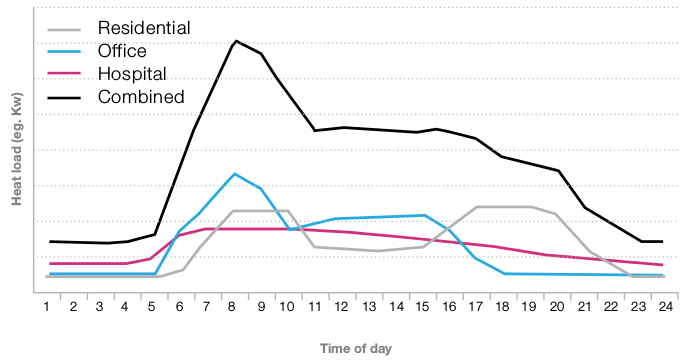
\includegraphics[width=0.5\linewidth]{mixLoad.png}
  \caption[Mixing Load Graph]{Mixing Load of Different Building
    Type~\cite{decentralHeatMap2011}}
  \label{fig:mixLoad}
\end{figure}

\subsection{More Detailed Description of Energy Behavior Supports
  Better Design}
A simple annual or monthly average cannot effectly represent the real
energy consumption behavior of an individual building and the whole
urban environment. In order to present this complicated behavior of
time-dependent energy demand, the time dimension is necessary.

This can be explained in a concrete example. Hospitals are usually
constant heat consumers with very stable heat demand throughout a year
(see \fref{fig:HG}), while a performance center is, on the other hand,
an occasional huge heat consumer with very high peak demand occuring
occasionally at event time and with almost zero demand in the
remaining time. It is reasonable to apply different energy planning
strategy for building groups involving one of these two types of
buildings. However, if time dimension is omitted, one has to choose
some aggregated description of the energy consumption of the two
building types, be it average, maximum, minimum or annual total. For
most cases, annual total demand is used for representing a building's
energy demand, especially in the case of District System design. With
this approach, the different energy usage pattern of a hospital and a
performance center might look the same, which results in a simplified
energy plan decision.

\subsection{Aggregation of Peak Value Becomes Tricky for Data with
  Time Variation}
One common mistake for sizing a district thermal energy system is to
add up the peak demand of each terminal users. Since the peak demand
of individual buildings do not occur at the same time, the end result
of summing up the peak demand at each end point exceeds the actual
total demand peak of the community. Hence with this approach, the
whole district system becomes excessively over-sized, which reduces
the whole system efficiency. A Dynamic Energy Map can reveal the
problem of such approaches by directly providing the aggregated
thermal energy and electricity demand for single buildings, building
sectors or the whole community. It allows a side by side comparison of
single building demand and aggregated demand and eliminates the
misunderstanding of the demand aggregation. With the direct
information of aggregated thermal energy and electricity demand, it
also assists actually sizing a district thermal energy system.




% Chapter 3

\chapter{Related Works} % Main chapter title

\label{Chapter2} % For referencing the chapter elsewhere, use \ref{Chapter1} 

\lhead{Chapter 2. \emph{Related Works}} % This is for the header on each page - perhaps a shortened title

%----------------------------------------------------------------------------------------

This section provide an overview of the existing instances of static
energy maps and dynamic energy maps. \sref{staticEnergyMap} and
\sref{dynamicMap} presents a general information of the energy mapping
instanceses. Then the summary of demand side information, supply side
information and techniques used to produce these Static and Dynamic
Energy Map instances are shown in \sref{summaryMap}.

\section{Static Energy Map}\label{staticEnergyMap}
\subsection{London Heat Map}
Under the goal of supplying 25\% of the total energy with
decentralized energy (DE) by the year 2025, the Decentralised Energy
Master Planning Program (DEMaP) was conducted between 2008 to 2010 to
``identify opportunities for district heating networks through heat
mapping and energy masterplanning''~\cite{londonHeatMap}. In this
study, the term DE only refers to ``combined heat and power systems
connected to district heating
networks''~\cite{decentralHeatMap2011}. 

London Heat Map is a publicly accessible interactive map developed as
part of the DEMaP project. It is completed for the London Boroughs in
2012. It can act as a starting point of Energy Master Plan for local
authorities, and can assist developers to make connections to existing
DE networks to meet policy requirements (London Plan DE
policy)~\cite{decentralHeatMap2011, londonHeatMap}. Point features of
high heating energy consumers and suppliers, existing and emerging
energy networks are depicted on the interactive map. High DE potential
regions (``focus area''~\cite{decentralHeatMap2011}) are identified
and depicted on the map to highlight the opportunities of utilizing
the heat supply in the community planning and development
(\fref{fig:londonHeat}). The ``live-database'' property of London Heat
Map allows new data of energy consumption be uploaded by users.

The criteria applied for identifying focus area include: 1) near to
existing or emerging DE network, 2) high heat demand density 3) anchor
load building, 4) diverse heating demand profile 5) has public
ownership with policy concerns to make connections to the DE
network~\cite{decentralHeatMap2011}. The physical constraint are also
considered in finalizing the high DE potential regions.

\begin{figure}[h!]
  \centering
  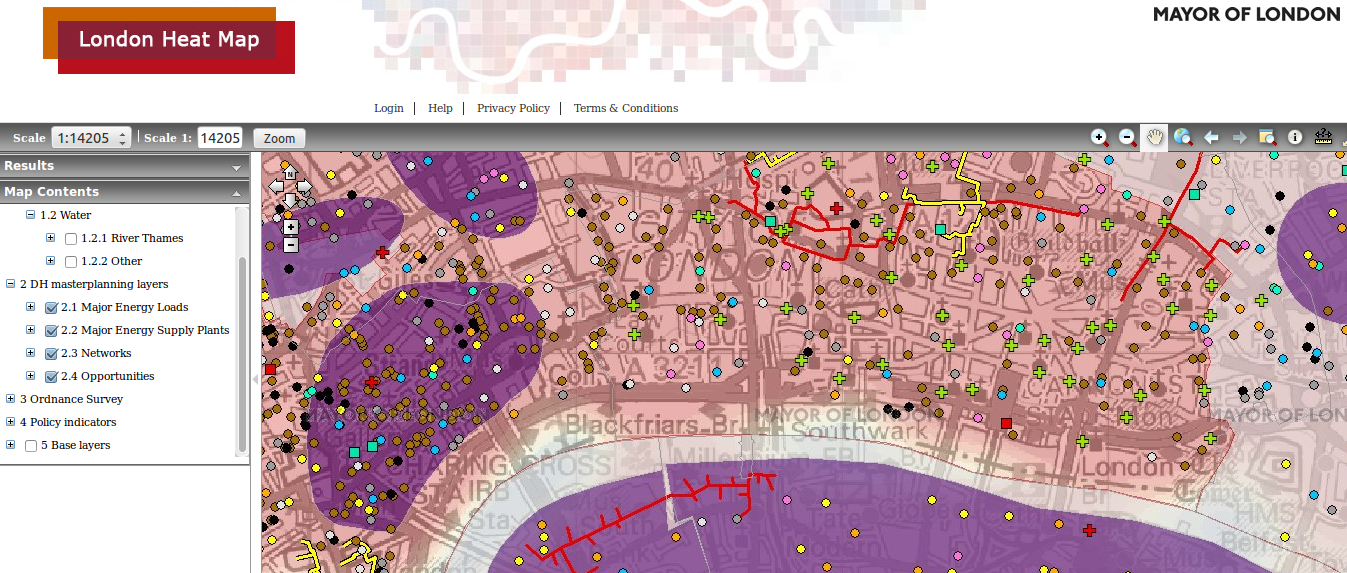
\includegraphics[width=0.7\linewidth]{londonHeat.png}
  \caption[London Heat Map]{London Heat Map~\cite{londonHeatMapMap}}
  \label{fig:londonHeat}
\end{figure}

\subsubsection{National Heat Map}
National Heat Map (\fref{fig:nhm}) is another UK energy mapping
project that focuses more on the industry
side~\cite{decentralHeatMap2011}. It is a ``high resolution
web-based'' heating energy interactive map, developed by the
Department of Energy and Climate Change (DECC). It aims at ``support
planning and deployment of local low-carbon energy projects in
England''~\cite{heatMap2015}. Power plant developers can use this map
to consider the feasibility for a CHP plant under policy
requirements~\cite{decentralHeatMap2011}. Heating demand density
($kWh/m^2$) of four major building sectors: public buildings,
commercial buildings, industry buildings and residential buildings,
together with the total demand is plotted on the map as a 2D raster
image with a discrete color scheme from blue to red representing low
to high heating demand. Heat source of CHP stations and thermal power
stations are plotted as point features in the map. Address level heat
demand data in csv format is also available for local authorities upon
request~\cite{heatMapLocal2012}.

\begin{figure}[h!]
  \centering
  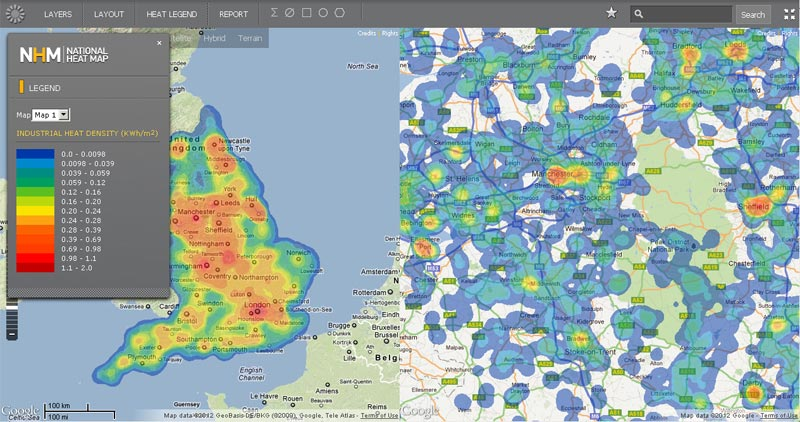
\includegraphics[width=0.5\linewidth]{nhm.jpeg}
  \caption[National Heat Map]{National Heat Map~\cite{heatMap2012}}
  \label{fig:nhm}
\end{figure}

\subsubsection{Water Source Heat Map}
The ``Water Source Heat Map'' (\fref{fig:waterMap}) is an added layer
group to the existing National Heat Map with information about the the
heat potential of the 4041 waterways in England. Heat potential of
waterways are represented in temperature, surface area, flow rate and
heat capacity ($kJ/m^3$ for coastal and estuary, $kW$ for canal, river
and settlement). It aims at supporting the plan of water-based thermal
system as water-based heat pump~\cite{waterHeatMap}. The map revealed
the large thermal capacity of water bodies that could serve over one
million buildings in the UK~\cite{waterHeatMap}.

\begin{figure}[h!]
  \centering
  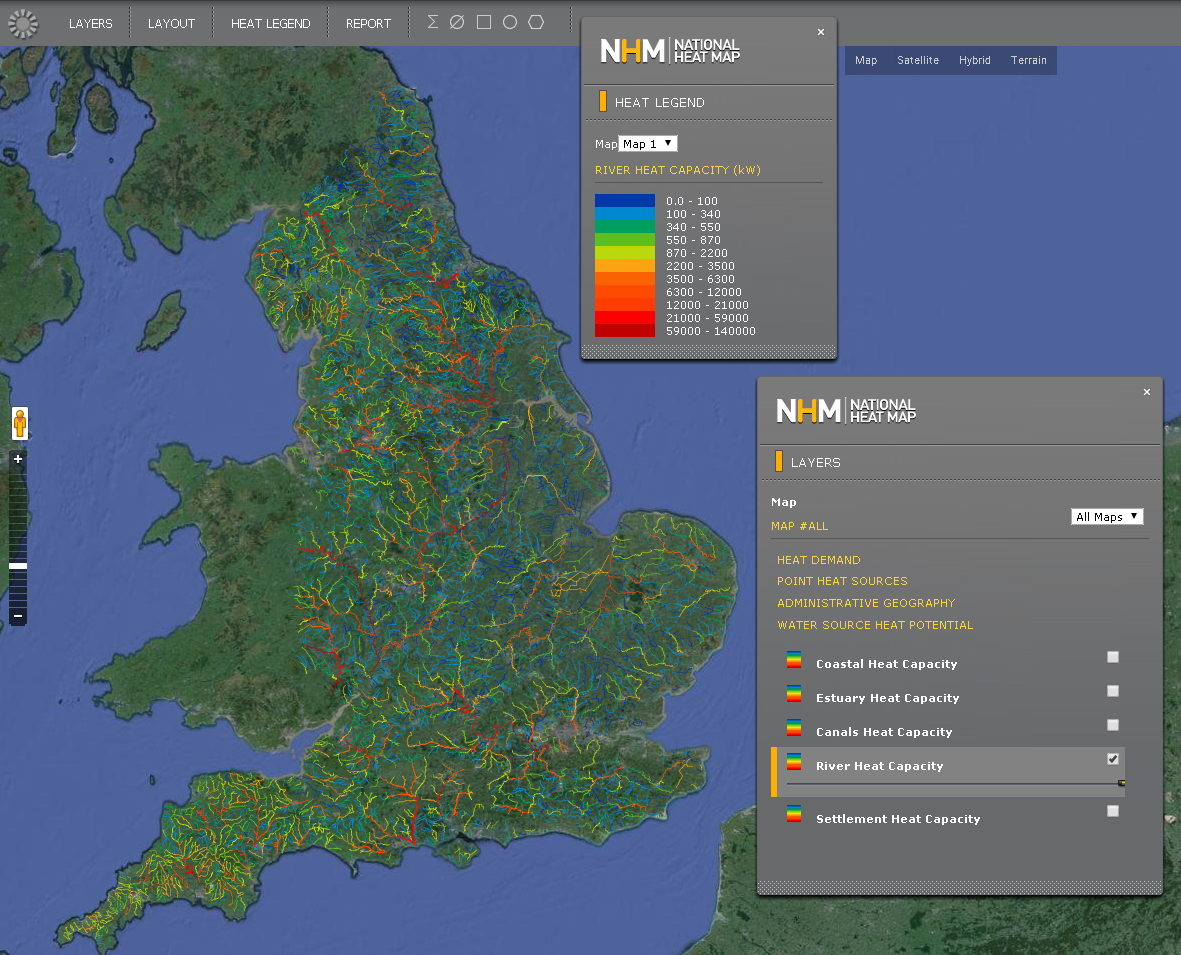
\includegraphics[width=0.5\linewidth]{waterMap.png}
  \caption[Water Heat Map]{Water Source Heat Map~\cite{waterHeatMap}}
  \label{fig:waterMap}
\end{figure}

\subsection{Calgary Energy Map}
One of the early instances of Static Energy Mapping is the Energy
Mapping Study of City of Calgary in 2008, carried out by Canadian
Urban Institute. It aims at providing insights to achieve the goal of
reducing 50\% of Green House Gas (GHG) emissions by
2050~\cite{aacip2009}. It depicts 1) how building design strategies
and land use planning can influence the city level energy use
intensity 2) the availability of alternative energy sources and the
opportunities to combine building level sustainable design technology
with the community level energy system design.

Calgary energy map first compares energy use intensity (the annual
total demand for thermal energy of space heating cooling, hot water
and electricity per unit area~\cite{aacip2009}) in GJ/ha between two
development cases: ``business as usual'' case and ``ultra-high
efficiency'' case (\fref{fig:calgaryCmp}). The comparison demonstrated
a 34\% reduction in energy use intensity from the former to the
latter~\cite{aacip2009}.

\begin{figure}[h!]
  \centering
  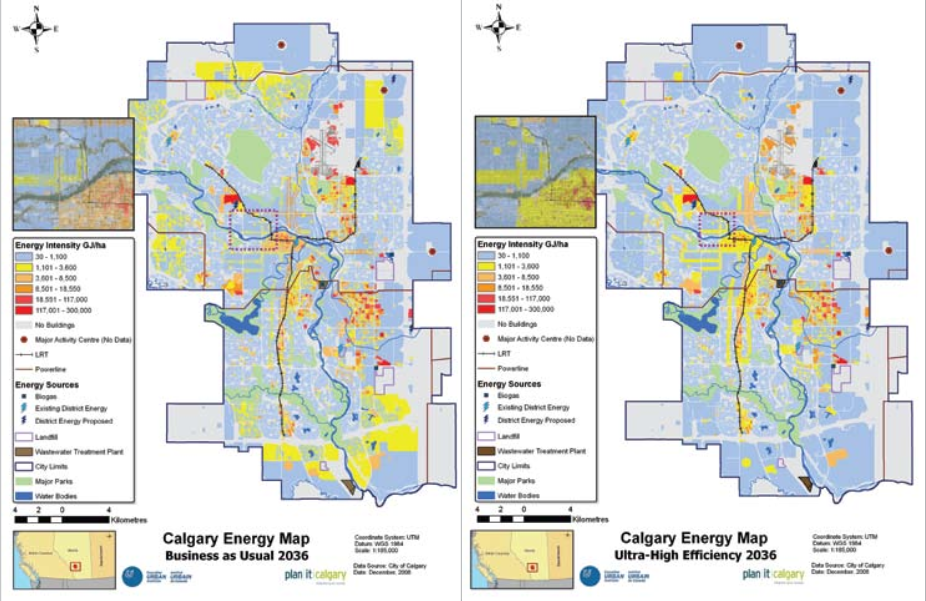
\includegraphics[width=0.6\linewidth]{calgaryCmp.png}
  \caption[Calgary Energy Demand Map]{Calgary Energy Map (Business as Usual, Ultra-High
    Efficiency)~\cite{aacip2009}}
  \label{fig:calgaryCmp}
\end{figure}

It also shows alternative energy sources of district energy, solar hot
water, solar air, energy sharing and PV installation on the map
(\fref{fig:calgaryAlter}). By overlaying the alternative technology
map and the ``ultra-high efficiency'' map, it highlights the
opportunities of using alternative renewable energy sources and
district energy system to further improve the energy performance of
high energy demand areas after high performance building design was
applied~\cite{aacip2009}.

\begin{figure}[h!]
  \centering
  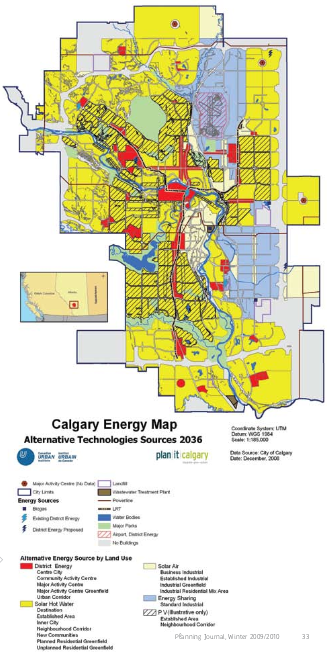
\includegraphics[width=0.3\linewidth]{calgaryAlter.png}
  \caption{Calgary Energy Map Alternative Energy Source~\cite{aacip2009}}
  \label{fig:calgaryAlter}
\end{figure}

\subsection{Energy Potential Mapping}
Dobbelsteen et al. described a framework of Energy Potential Mapping
(EPM) that aggregates information of energy supply, demand and
infrastructure on the same map with demand and supply represented in
the same unit of GJ or GJ/ha~\cite{Dobbelsteen2013}.

In 2010, a ``Heat Mapping'' study under the framework of EPM was
launched by TU Delft aiming at visualizing heat demand and supply and
infrastructure with the same unit that facilitates easy comparison and
facilitates the matching of supply and
demand~\cite{Dobbelsteen2013}. The map is presented with aggregated
supply and demand in a 3D Heat Map. The absolute quantity of each type
of demand and supply is represented with extruded height in the 3D
map. Demand is represented with a transparent 3D feature, and each
supply source is represented with solid 3D feature in a different
color~\cite{Dobbelsteen2013}.

\begin{figure}[htbp]
  \centering
  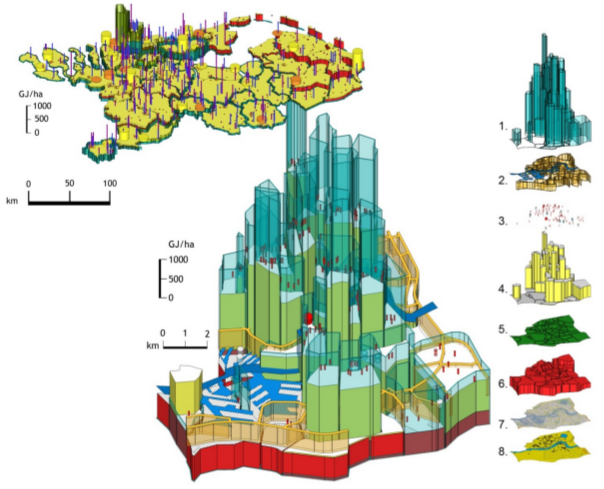
\includegraphics[width=0.7\linewidth]{heatmapNL.png}
  \caption[Rotterdam Heat Map]{Heat Mapping of Netherlands and
    Rotterdam~\cite{Dobbelsteen2013}}
  \label{fig:heatmapNL}
\end{figure}

\section{Dynamic Energy Map}\label{dynamicMap}
Per definition of Dynamic Energy Map in the introduction, there are
not instances that fully realized all the desired functions yet. In
this section, some valuable attempts towards realizing and exploring
the power of dynamic energy mapping will be discussed.

\subsection{Lower Hill District Dynamic Mapping Project}
In 2011 to 2012, the Dynamic Energy Map of the Lower Hill District,
Pittsburgh, PA was created. It is designed to conduct feasibility
analysis and comparison of alternative energy supply techniques of a
district energy system~\cite{baird2014, Ramesh2013}. A geo-data base
was created with ArcMap, ArcScene and Sketchup. In the database, each
building, represented as a 3D feature, contains attributes of its
building name, annual energy consumption, energy use intensity (EUI),
and annual and monthly peak demand. The map is online accessible via
GIS Cloud (\fref{fig:mellonArenaGIS}).

\begin{figure}[h!]
  \centering
  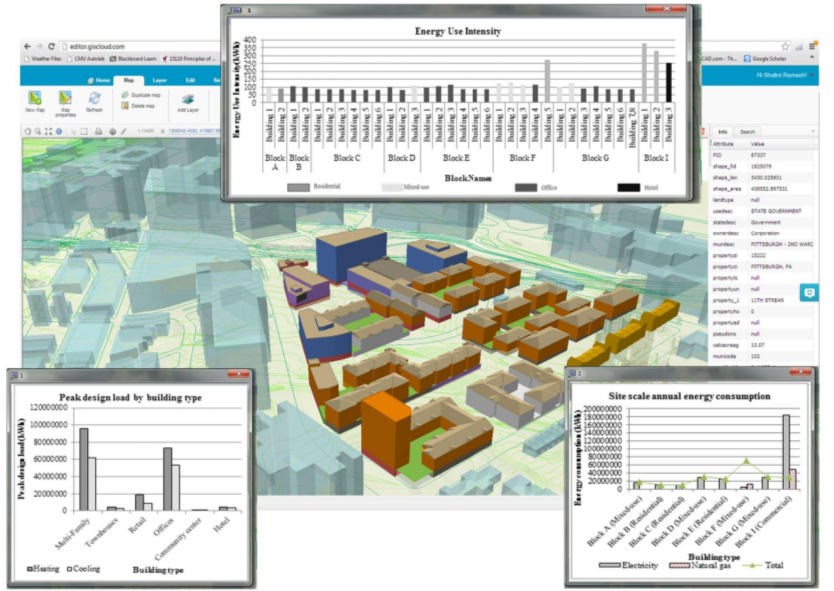
\includegraphics[width=0.7\linewidth]{mellonArenaGIS.png}
  \caption[Lower Hill District 3D GIS Map]{Online Accessible GIS-database with GIS
    Cloud~\cite{baird2014, Ramesh2013}}
  \label{fig:mellonArenaGIS}
\end{figure}

The feasibility analysis and temporal data display are separated from
the geo-database and is performed in a excel screening tool. The tool
takes input of energy cost rate, building type and size, development
phase and central plant types and feature and produces a feasibility
analysis and related temporal graphs (\fref{fig:3dexcel}) of annual
hourly energy consumption for each building type and the aggregated
demand of natural gas, cooling use electricity and total electricity.

\begin{figure}[h!]
  \centering
  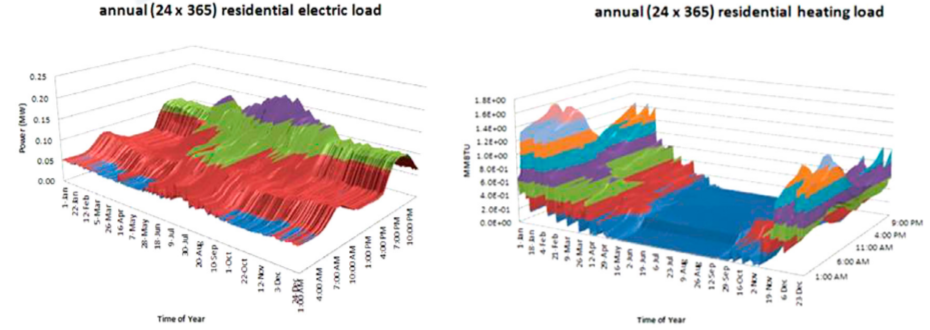
\includegraphics[width=0.7\linewidth]{3dexcel.png}
  \caption[Heating/Electricity Residential]{Heating Load and
    Electricity Load for Residencial Building~\cite{baird2014}}
  \label{fig:3dexcel}
\end{figure}

\subsection{Energy Mapping to Identify Opportunities for Future
  Networks Project (EMIOFN)}
Another instance of energy demand dynamic map with high spatial
resolution was found in the project ``Energy Mapping to Identify
Opportunities for Future Networks''~\cite{Diaz2013}. The aim of the
project is to ``analyze the spatial and temporal distribution of
energy consumption'' and support decision making and design of energy
network: more specifically, to identifiy opportunities of District
Heating, CHP plant development and Building Design
Improvement~\cite{Diaz2013}.

Energy Demand Maps of three different resolutions were created using
QGIS: campus level, community level and city level. Energy data was
retrieved from both metered data (used in campus level map) and HEM
simulation (used in community and city level map). HEM is a tool for
``mapping the possiblemapping the possible carbon and energy
performance of a dwelling. It has pre-simulated results embedded as a
data table in the tool and applies the appropriate system and context
calculations to provide instant energy, carbon and cost results''~\cite{HEMesru2015}.

For the campus level map, the heat demand density (heat demand over
conditioned area) were depicted to identify ``outliers'': the
buildings with high heat demand~\cite{Diaz2013campus}. These outliers
were potential buildings need to be improved in building insulation
level or HVAC system efficiency. They claim a spatial map is
sufficient for this outlier identification process
(\fref{fig:heatGlasgow}). They also created a temporal spatial map of
monthly heat consumption that is in the form of both small multiples
(\fref{fig:seqheatGlasgow}) and non-interactive animated map
(\fref{fig:animeheatGlasgow}). With the dynamic map, they identified
two campus buildings with high heat demand through the whole year
(anchor load building) and concluded that the two buildings could
connect to a district heating system. They also created two animated
maps with electricity and natural gas. By comparing these two animated
maps, consistent high consumers for electricity and gas were
identified as potential candidate building for a micro-CHP
system~\cite{microCHP}.

\begin{figure}[h!]
  \centering
  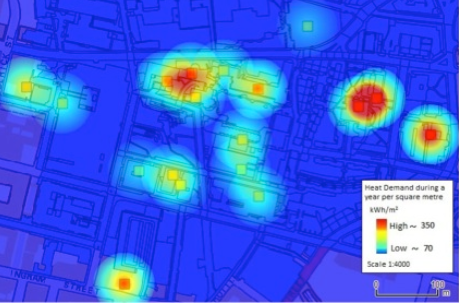
\includegraphics[width=0.5\linewidth]{heatGlasgow.png}
  \caption[Heat Demand Density]{Campus Level Heat Demand Density Map~\cite{Diaz2013campus}}
  \label{fig:heatGlasgow}
\end{figure}

\begin{figure}[h!]
  \centering
  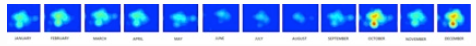
\includegraphics[width=0.5\linewidth]{seqheatGlasgow.png}
  \caption[Monthly Heat Demand (Small Multiple)]{Campus Level Monthly Heat Demand Map in Small Multiples\cite{Diaz2013campus}}
  \label{fig:seqheatGlasgow}
\end{figure}

\begin{figure}[h!]
  \centering
  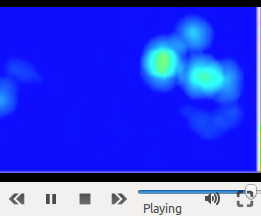
\includegraphics[width=0.3\linewidth]{animeheatGlasgow.png}
  \caption[Campus Animated Map]{Campus Level Monthly Heat Demand Map in Animation\cite{Diaz2013campus}}
  \label{fig:animeheatGlasgow}
\end{figure}

The community level spatial and temporal GIS analysis undertook a
similar process as the campus level except for the energy data is
retrieved from HEM simulation. By comparing the four different
building types: ``Traditional Build, New Build, Council Estate, High
Rise Flat'', they identified the consistent high gas and electricity
demand of High Rise Flat buildings. They also discovered that the
improvement of building design could adjust the heat to power ratio
(HTP) and could make applying CHP option feasible~\cite{Diaz2013com}.

\section{Summary}\label{summaryMap}
\subsection{Demand Side Information}
\tref{tab:demandInfo} summarizes the energy demand topics of the cases
presented in this section. The demand information presented in all
cases is heat demand except that the Calgary map has information of
the total energy demand: the sum of heating cooling and electricity
demand. The demand time resolution is year (represented as annual
total or annual total density) or month (monthly peak or monthly
total) for almost all instances, except that the Lower Hill District
Project screening tool has hourly demand information in the screening
tool.

\begin{table}[h!]
\centering
\caption{Demand Side Input Information}
\label{tab:demandInfo}
\begin{tabular}{p{3cm}|p{3cm}|p{3cm}|p{3cm}}
  \hline
  Project                 & Demand Topic                                             & Time                                        & Unit                      \\
  \hline
  \hline
  London Heat Map         & heat demand                                              & annual total density                                & kWh/m2 per year           \\
  \hline
  National Heat Map       & heat demand                                              & annual total density                                & kWh/m2 per year           \\
  \hline
  Water Source Heat Map   & x                                                        & x                                           & x                         \\
  \hline
  Calgary Map             & sum of space heating, cooling, hot water and electricity & annual total density                                & GJ/ha per year            \\
  \hline
  Dutch Heat Map          & heat demand                                              & annual total density                                & GJ/ha per year            \\
  \hline
  Lower Hill District Map & heat demand and electricity demand                       & Geo-database: annual total density, annual total and monthly peak & kBtu/ft$^2/year$ for EUI, kBtu for annual total, Btu/hr for peak demand \\ 
  \cline{3-4}
                          &                                                          & Screening tool: hourly                      & MW for electricity demand, MMBtu for heat demand     \\
  \hline
  EMIOFN                  & heating and cooling demand                                              & annual total density and monhly total              & kWh/m2 per year          \\
  \hline
\end{tabular}
\end{table}

The information included in my dynamic energy map is similar to that
of Calgary energy map: space heating, cooling, hot water and
electricity demand are depicted on the map. Calgary map has a single
layer of total demand, while my dynamic energy map provide single
layers of heating, cooling and electricity demand over time, as well
as two bivariate map layers: a bivariate layer of space heating and
cooling demand and a bivariate layer of heating demand and electricity
demand. The bivariate layer of space heating and cooling demand can
help users identify energy recovery opportunities
(\fref{fig:heatcool}). The bivariate layer of heat and power
accompanied with the aggregated heating and electricity data plot can
help users identify help the sizing of community district system CHP
plant(\fref{fig:heatpower}). Data plot of heating, cooling and
electricity of the community and single buildings in the community are
also provided to anchor quantitative information
(\fref{fig:heatCoolElec}).

\begin{figure}[h!]
  \centering
  \begin{subfigure}{0.4\textwidth}
  \centering
  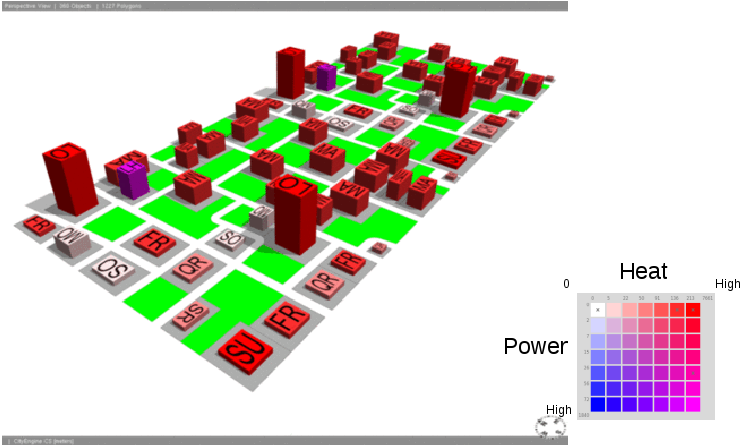
\includegraphics[width=\linewidth]{heatcool.png}
  \caption[Bivariate Layer of Heating and Cooling]{3D bivariate layer
    of space heating and space cooling demand}
  \label{fig:heatcool}
\end{subfigure}
~
\begin{subfigure}{0.4\textwidth}
  \centering
  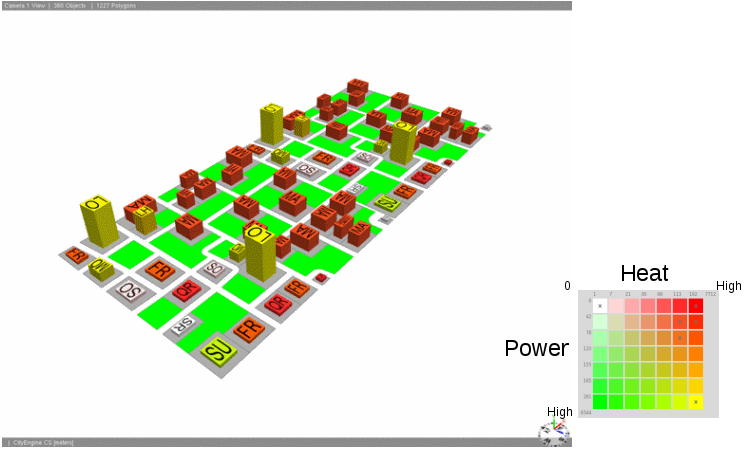
\includegraphics[width=\linewidth]{heatpower.png}
  \caption[Bivariate Layer of Heating and Electricity]{3D bivariate
    layer of heating and electricity demand}
  \label{fig:heatpower}
\end{subfigure}
\caption[Comparing Heating:Gas and Space Heating]{Comparing
  Heating:Gas and Space Heating}
\end{figure}

\begin{figure}[h!]
  \centering
  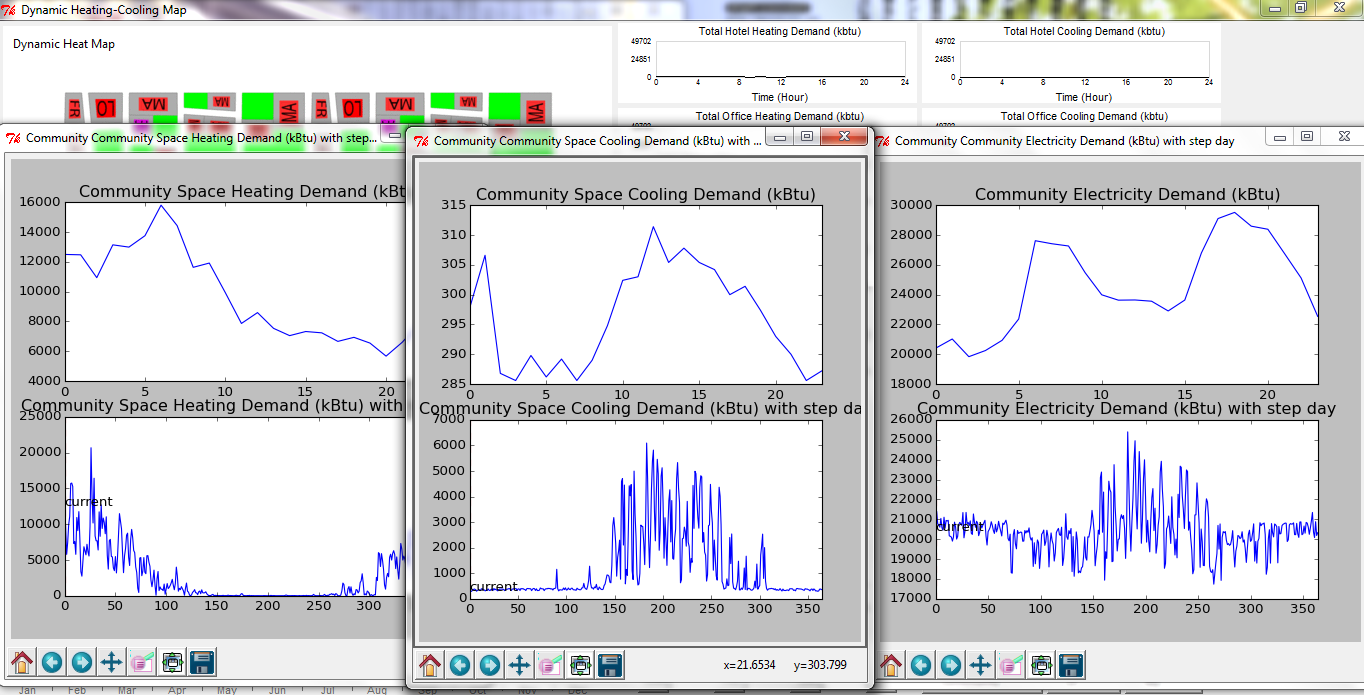
\includegraphics[width=0.5\linewidth]{heatCoolElec.png}
  \caption[Plot of Heating, Cooling and Electricity]{The example shows
    the plot of heating, cooling and electricity demand of the Large
    Office}
  \label{fig:heatCoolElec}
\end{figure}

Comparing with the static and dynamic map instances, which all use
annual / monthly total / total density as the indicator for energy
demand except that the screening tool in the Lower Hill District
Project has hourly demand information. My dynamic energy map adopts
the time resolution as the screening tool in the Lower Hill District
Project. It contains hourly energy demand data for every single
building and the community. Sizing of a district system requires peak
thermal energy demand of the community. This variable is missing from
all the existing static maps. My dynamic energy map shows the total
heat and electricity demand as plot on the interface and the users can
use this information to size a district energy system
(\fref{fig:CHPHeating}). 

% plot of aggregate demand (heating)
\begin{figure}[h!]
  \centering
  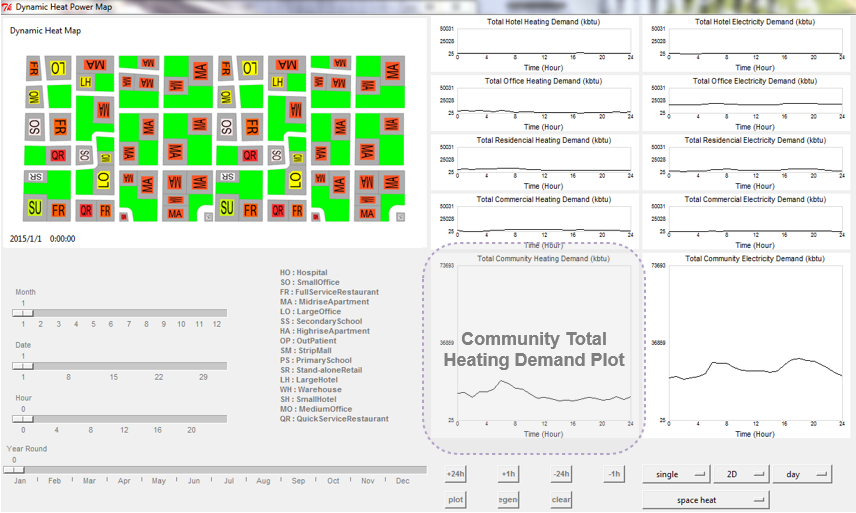
\includegraphics[width=0.7\linewidth]{CHPHeating.png}
  \caption[Plot of Heating, Cooling and Electricity]{Plot of Heating, Cooling and Electricity}
  \label{fig:CHPHeating}
\end{figure}

I chose to represent energy demand as absolute value rather than
density value in order to provide quantitative information for the
amount of energy that could be recovered within building groups or
communities and to provide information for the total thermal energy
demand in order to size system capacity of a CHP plant. 

My dynamic energy map also provide different forms of energy data
aggregation over the time dimension, such as total, peak and average
demand over a year, a month a week or a day (\fref{fig:aggOption}).
% plot of aggregate total, ave, peak etc.
\begin{figure}[h!]
  \centering
  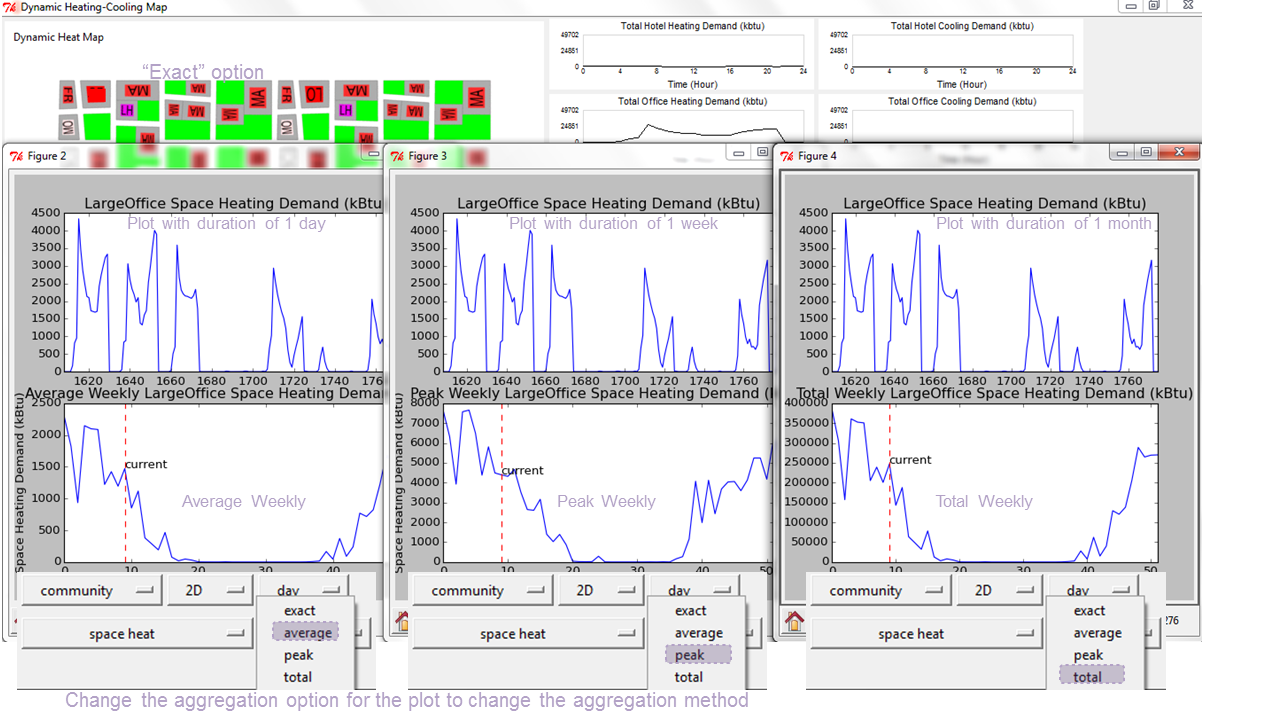
\includegraphics[width=0.7\linewidth]{aggOption.png}
  \caption[Plot of Different Energy Aggregation Method]{Plot of Different Energy Aggregation Method}
  \label{fig:aggOption}
\end{figure}

\subsection{Map Representation}\label{sec:mapRepre}
\tref{tab:mapRep} summarizes the data representation method used in
the cases presented in this section.

\begin{table}[h!]
\centering
\caption{Map Representation of Related Works}
\label{tab:mapRep}
\begin{tabular}{p{4cm}|p{4cm}|p{4cm}}
  \hline
  Project                 & Geometry                            & Quantity representation         \\
  \hline
  \hline
  London Heat Map         & point                               & graduated symbol size           \\
  \hline
  National Heat Map       & raster                              & discrete graduated color ramp (blue to red with red for high heat demand) \\
  \hline
  Water Source Heat Map   & x                                   & x                               \\
  \hline
  Calgary Map             & polygon                             & discrete graduated color ramp  (blue to red with red for high energy demand) \\
  \hline
  Dutch Heat Map          & extruded polygon                    & height of polygon               \\
  \hline
  Lower Hill District Map & Geo-database: 3D building and site  & Bar Chart                       \\
  \cline{2-3}
                          & Screen Tool: no geometry associated & Screening Tool: 3D height graph \\
  \hline
  EMIOFN                  & raster                              & continuous graduated color (blue to red with red for high heat demand) \\
  \hline
\end{tabular}
\end{table}

In London Heat Map, locations of potential heat consumers are
aggregated to point features on each building centroid. The annual
total heating energy demand (MWh per year) is represented with the
graduated size of the point symbol (\fref{fig:londonHeatMapDmd}).

In Calgary Energy Map, the total demand of heating, cooling, service
hot water and electricity are represented as area density in
$GJ/ha$. The demand layer is a polygon feature layer with energy
demand density represented as a graduated color symbol from blue to
red.

In National Heat Map and Water Source Heat Map, the heating demand in
$kWh/m^2$ is depicted with a raster density map layer. The same
approach of using the density raster layer to represent heating and
electricity demand is adopted by the EMIOFN project.  Raster density
maps are helpful in removing clutter in small-scale maps that depicts
large regions (\fref{fig:nhm4London}). For large-scale maps, the
National Heat Map provides multiple views so that the raster heat
demand density map can be visualize side by side with the satellite
view to provide the urban environment context.
\begin{figure}[h!]
  \centering
  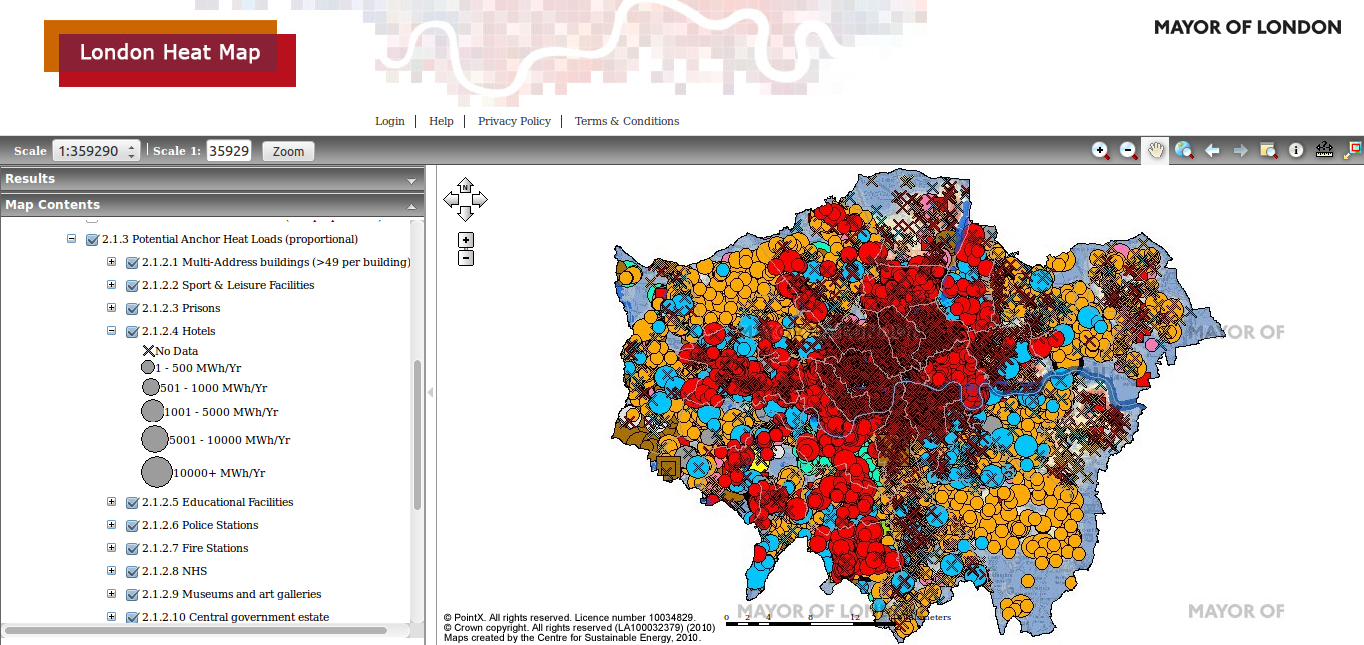
\includegraphics[width=0.7\linewidth]{londonHeatMapDmd.png}
  \caption[London Heat Map with Graduated Point Feature]{London Heat
    Map with Graduated Point Feature~\cite{londonHeatMapMap}}
  \label{fig:londonHeatMapDmd}
\end{figure}
~
\begin{figure}[h!]
  \centering
  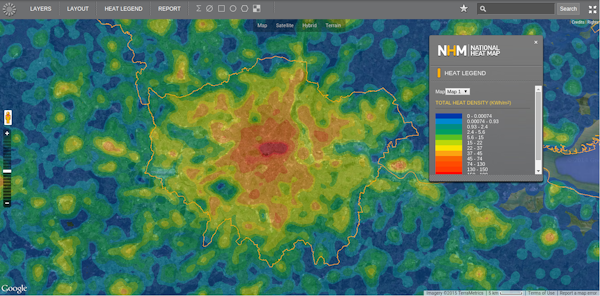
\includegraphics[width=0.7\linewidth]{nhm4London.png}
  \caption[National Heat Map for London]{National Heat Map that
    depicts the region of London~\cite{londonHeatMapMap}}
  \label{fig:nhm4London}
\end{figure}

Dutch heat map uses the same density map approach but the density is
not interpolated over space as in National Heat Map and EMIOFN. It is
represented as the height of the building or region.

The Lower Hill District Map does not directly represent energy demand
on the 3D map geometry, it uses an attribute table and bar chart to
visualize the demand quantity.

My dynamic energy map does not took the raster density map approach
because raster density map or graduated size symbol because the former
creates a 3D geometry layer and the latter create too much shape
distortion. Both approaches will impair my goal of representing a
realistic urban environment since the current map only contains one
map display window. These approaches could become valid in further
development of my current map so that it provide two side-by-side
window that shows the urban context and the energy demand layer in
different display window as in the example of National Heat Map
(\fref{fig:twoWindow}).

\begin{figure}[h!]
  \centering
  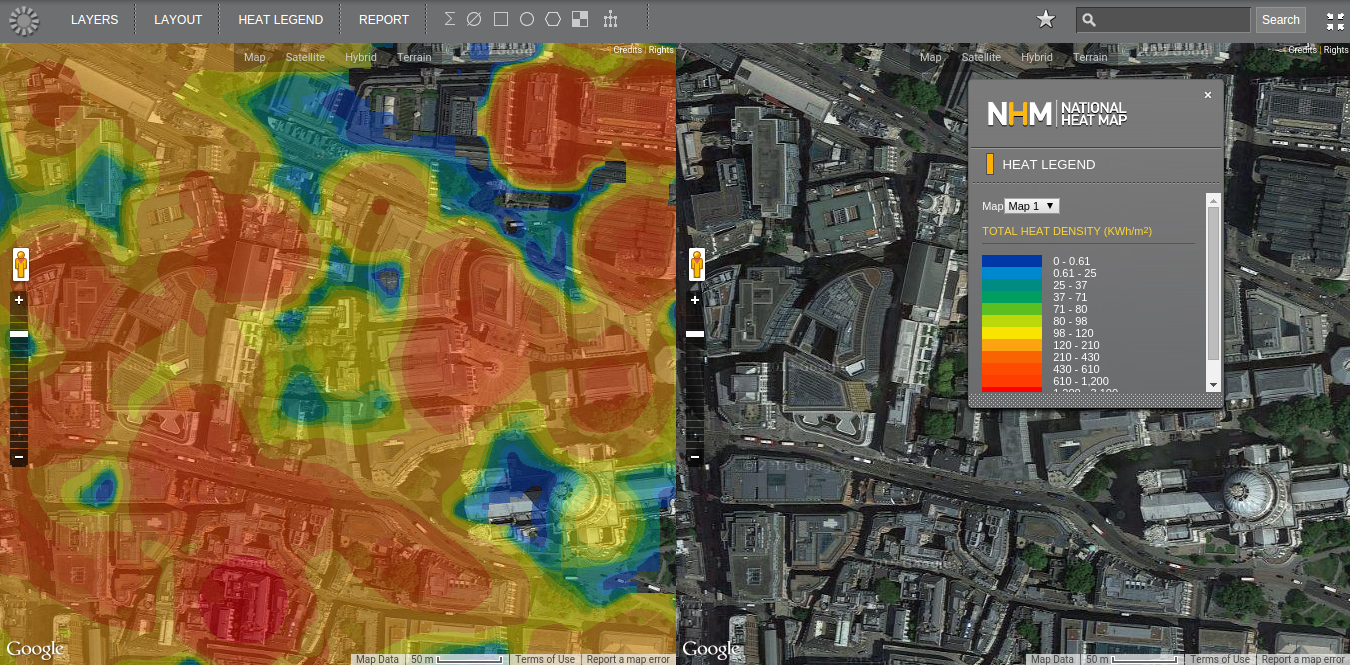
\includegraphics[width=0.7\linewidth]{twoWindow.png}
  \caption[Two Window Display of National Heat Map]{National Heat Map
    depicts the heating energy demand on the left and the urban
    environment context on the right~\cite{londonHeatMapMap}}
  \label{fig:twoWindow}
\end{figure}

\subsection{Techniques used}
The Calgary Map, Dutch Heat Map and EMIOFN map are stand-alone maps
produced with desktop GIS software. London Heat Map, National Heat
Map, Water Source Heat Map and Lower Hill District project are on-line
maps accessible through browsers. 

With limited software survey of ArcGIS and CityEngine, existing GIS
software are not capable of implementing an efficient dynamic energy
map. The major weakness is in the energy data visualization and the
high requirement of computational power. The limitations of existing
tools are summarized in \sref{sec:aggregateTime}. The tool used in the
implementation of the current dynamic energy map is
Python~\cite{python2015} with the Tkinter package~\cite{Tkinter2014}
for UI design and the pandas~\cite{pandas2015},
NumPy~\cite{NumPy2015}, Matplotlib~\cite{matplotlib2015} and
ggplot~\cite{ggplot2015} for database functions and data plot
creation. ImageMagick~\cite{ImageMagick2015} is used in image
formating and resizing. FFmpeg ~\cite{FFmpeg2015} is used in
connecting image sequences to animations.

\begin{table}[h!]
\centering
\caption{Map Technology Summary Table}
\label{tab:mapSummary}
\begin{tabular}{p{3cm}|p{3cm}|p{3cm}|p{3cm}}
  \hline
Project                 & Type    &             & Software                                  \\
  \hline
  \hline
London Heat Map         & Static  & web         & ArcGIS WebApp                             \\
  \hline
National Heat Map       & Static  & web         & Google Map API                            \\
  \hline
Water Source Heat Map   & Static  & web         & Google Map API                            \\
  \hline
Calgary Map             & Static  & stand-alone & ?                                         \\
  \hline
Dutch Heat Map          & Static  & stand-alone & ?                                         \\
  \hline
  \hline
Lower Hill District Map & Dynamic & web         & Map Creation: ArcScene, ArcMap, GIS Cloud \\
                        &         &             & Energy Simulation: EnergyPlus             \\
  \hline
EMIOFN                  & Dynamic & stand-alone & QGIS (Map Creation)                       \\
                        &         &             & HEM (Energy Simulation)                  \\
  \hline
\end{tabular}
\end{table}

\subsection{Building from the Lower Hill District Project}
My current work builds directly on the Lower Hill District Project. As
is mentioned in the introduction, the major functions of a dynamic
energy map is: holding, visualizing and analyzing community level high
spatial-temporal resolution energy demand and supply data and
connecting to simulation engine for dynamic performance analysis.

In the GIS map of the Lower Hill District Project by Baird et al.\
~\cite{baird2014}, holding spatial-temporal (although with low
temporal resolution) energy data and connecting to simulation software
is realized by processing the energy simulation data with Microsoft
excel and importing the csv file including ``building name, total
conditioned area annual, energy use intensity, annual and monthly peak
demand''. My dynamic energy map builds on this and makes the
geo-database hold more high resolution energy data imported from
EnergyPlus simulation, meaning the 8760 hourly energy data should be
contained in the dynamic energy map.

The feasibility analysis of a district energy system is performed in a
stand-alone Excel tool~\cite{baird2014}. My further improvement is to
aggregate part of the function of the screening tool, the calculation
and display of aggregated total heating and electricity demand, into
the dynamic energy map.

The spatial and temporal information are visualized separately in the
Lower District Hill Project: the spatial information of 3D building
geometry and location could be visually inspected in the GIS map but
not the hourly energy consumption information; the temporal
visualization of energy demand is done separately in the Excel
screening tool as 3D graphs, but no spatial context is present and the
spatial dimension is then lost. My improvement is to create a set of
spatial-temporal energy data display system that can better convey the
energy demand changes over space and time.
% Chapter 4

\chapter{Methodology} % Main chapter title

\label{Chapter4} % For referencing the chapter elsewhere, use \ref{Chapter1} 

\lhead{Chapter 4. \emph{Drawings}} % This is for the header on each page - perhaps a shortened title

%----------------------------------------------------------------------------------------
\section{Overview}
The Dynamic Energy Map is created for a conceptual urban environment
with the following properties:
\begin{enumerate}[i.]
\item Of realistic building density and land use pattern.
  
  To achieve this, the current study used a redevelopment project at
  Lower Hill District, Pittsburgh, PA~\cite{Ramesh2013} as a
  prototype.  The land use of the conceptual urban environment is
  created based on extracted topological patterns from this
  redevelopment projec.

\item The number of buildings in the model represents a typical
  community that can be served by a district energy
  system~\cite{IDEA2012}.
  
  To achieve this, the original model created under crateria i. is
  duplicated and thus there are in total 68 buildings within the
  community. This rangge is within the range of a typical district
  energy system service capacity of 50 to 150~\cite{IDEA2012}.

\end{enumerate}

The inputs to the dynamic energy map include the hourly energy
consumption data and the urban environment layout. For the conceptual
setting, the energy data is retrieved from the simulation of DOE
Benchmark buildings of new construction which comply with ASHRAE
90.1-2004 Standard~\cite{DOE2015}.

The output of the dynamic energy map is a sequence of 2D or 3D energy
choropleth map images.

An interface is designed to provide an interactive inspection of the
map image sequence and the corresponding energy data plot of a single
buildings, building groups and the community that assists:
\begin{enumerate}[i.]
\item Comparing heating and cooling demand to identify energy recovery
  opportunities
\item Comparing heating and electricity demand to size co-generation
  system
\end{enumerate}

By replacing the simulated hourly energy demand data with actual
metered energy consumption data and the conceptual layout with a real
urban environment layout, the same method can be directly applied to
the analysis of a real project.

\begin{figure}[h!]
  \centering
  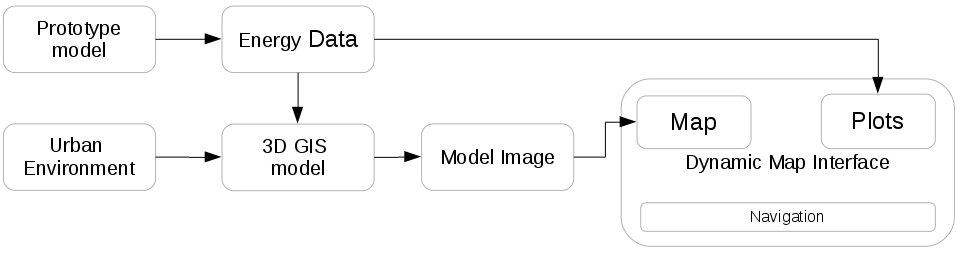
\includegraphics[width=0.7\linewidth]{flow.png}
  \caption[General Work Flow]{General Work Flow}
  \label{fig:flow}
\end{figure}

Details in input output data and the interface design process will be
explained in more details in the following sections.
\newpage
\section{Input}
\subsection{Benchmark Models and Energy Data}
In the Lower Hill District project, the DOE benchmark buildings were
substituted for buildings in the community model in the district
system feasibility analysis. This approach allows for a fast initial
assessment of the district system~\cite{baird2014}.

Following the same approach, the energy profile used in the current
study is retrieved from simulation results of commercial building
benchmark buildings developed by U.S. Department of Energy
(DOE)~\cite{DOE2015}. There are 16 building types in the benchmark
models (\fref{tab:doeModel}). The building types involved in the
current project include: Large Office (LO), Medium Office (MO), Small
Office (SO), Stand-alone Retail (SR), Supermarket (SU), Quick Service
Restaurant (QR), Full Service Restaurant (FR), Large Hotel (LH) and
Midrise Apartment (MA). The two-letter shorthand in the parenthesis
after each building type is used in the building label for the dynamic
map display. The general information for the benchmark buildings are
shown in \tref{tab:doeModel}:

\begin{table}[h!]
  \centering
  \begin{tabular}{l|l|c|c}
    \hline
Building Type Name&Shorthand&  Floor Area (ft2)    & Number of Floors\\
    \hline
Large Office	         &LO&  498,588	      & 12\\
Medium Office	         &MO&  53,628	      & 3\\
Small Office	         &SO&  5,500	      & 1\\
Warehouse	         &WH&  52,045	      & 1\\
Stand-alone Retail       &SR&  24,962	      & 1\\
Strip Mall	         &SM&  22,500	      & 1\\
Primary School	         &PS&  73,960	      & 1\\
Secondary School         &SS&  210,887	      & 2\\
Supermarket	         &SU&  45,000	      & 1\\
Quick Service Restaurant &QR&  2,500          & 1\\
Full Service Restaurant  &FR&  5,500          & 1\\
Hospital	         &HO&  241,351	      & 5\\
Outpatient Health Care   &OP&  40,946	      & 3\\
Small Hotel	         &SH&  43,200	      & 4\\
Large Hotel	         &LH&  122,120	      & 6\\
Midrise Apartment        &MA&  33,740	      & 4\\
    \hline
\end{tabular}
\caption{DOE Benchmark Building General Information~\cite{DOE2015}}
\label{tab:doeModel}
\end{table}

The benchmark buildings comply with the ASHRAE Standard 90.1-2004. The
HVAC system types are shown in \tref{tab:hvac}. The major heating
systems of the benchmark buildings are furnace and boilers, except
that the small hotel and the warehouse has individual space heaters
other than furnaces. The cooling systems are chillers for Large Hotel
(air-based) and Large Office (water-based) and PACU (packed
air-conditioning unit) for other building types.~

\begin{table}[h!]
\centering
\scriptsize
\caption{Benchmark Building HVAC System}
\label{tab:hvac}
%\begin{tabular}{l|p{3cm}|p{4cm}|p{4cm}}
\begin{longtable}{p{2cm}|p{2cm}|p{4cm}|p{4cm}}
  \hline
  & Heating                                & Cooling                                                                     & Air                                                     \\
  \hline
  \hline
  Small Office             & Furnace                                & PACU (packed air-conditioning unit)                                         & SZ CAV (single-zone constant air volume)                \\
  \hline
  Medium Office            & Furnace                                & PACU (packed air-conditioning unit)                                         & MZ VAV (multizone variable air volume)                  \\
  \hline
  Large Office             & Boiler                                 & Chiller (2) water cooled                                                    & MZ VAV (multizone variable air volume)                  \\
  \hline
  Primary School           & Boiler                                 & PACU (packed air-conditioning unit)                                         & CAV (constant air volume)                               \\
  \hline
  Secondary School         & Boiler                                 & Chiller (2) air cooled                                                      & MZ VAV (multizone variable air volume)                  \\
  \hline
  Stand-Alone Retail       & Furnace                                & PACU (packed air-conditioning unit)                                         & SZ CAV (single-zone constant air volume)                \\
  \hline
  Strip Mall               & Furnace                                & PACU (packed air-conditioning unit)                                         & SZ CAV (single-zone constant air volume)                \\
  \hline
  Suprmarket               & Furnace                                & PACU (packed air-conditioning unit)                                         & SZ CAV (single-zone constant air volume)                \\
  \hline
  Quick Service Restaurant & Furnace                                & PACU (packed air-conditioning unit)                                         & CAV (constant air volume)                               \\
  \hline
  Full Service Restaurant  & Furnace                                & PACU (packed air-conditioning unit)                                         & SZ CAV (single-zone constant air volume)                \\
  \hline
  Small Hotel              & ISH (individual space heater), furnace & IRAC (individual room air conditioner), PACU (packed air-conditioning unit) & SZ CAV (single-zone constant air volume)                \\
  \hline
  Large Hotel              & Boiler                                 & Chiller (2) air cooled                                                      & FCU (Fan Coil Unit) and VAV (variable air volume)       \\
  \hline
  Hospital                 & Boiler                                 & Chiller (2) water cooled                                                    & CAV (constant air volume) and VAV (variable air volume) \\
  \hline
  OutPatient Healthcare    & Furnace                                & PACU (packed air-conditioning unit)                                         & CAV (constant air volume) and VAV (variable air volume) \\
  \hline
  Warehouse                & ISH (individual space heater), furnace & PACU (packed air-conditioning unit)                                         & SZ CAV (single-zone constant air volume)                \\
  \hline
  Midrise Apartment        & Furnace                                & PACU-SS                                                                     & SZ CAV (single-zone constant air volume)               \\
  \hline
\end{longtable}
\end{table}

\pagebreak
\subsubsection{Input for Identifing Energy Recovery
  Opportunities}\label{sec:inputRecover}
The major heat rejection sources include heating mode heat rejection
and cooling mode heat rejection. The heat rejection in heating mode
happens during the process of the mixing of conditioned and outside
air. This source of heat rejection is more difficult to capture and is
thus left out from the energy recovery potential calculation in this
study. The current study will only focus on the cooling induced heat
reject. 

The heat rejection in cooling mode happens during the condensing
process when the high temperature refrigerant gas condenses with one
of the following heat rejection forms~\cite{Bhatia2015}:
\begin{itemize}
\item Air cooled unit: ambient air is blown through condensing coils
  and removes heat from the gas refrigerant.
\item Cooling tower: cooled water flow past the condensing unit and
  takes away the heat from the gas refrigerant. The water is then
  cooled through evaporation.
\item Fluid cooler: water is sprayed on the condensing coil with fan
  forced air flowing in the opposite direction. It causes evaporative
  cooling effect that takes away the heat from the gas refrigerant.
\end{itemize}
The ``condenser total heat of rejection''~\cite{Bhatia2015} (THR) in
the condensing process equals to the ``net refrigeration effect''
~\cite{Bhatia2015}(RE, the hourly cooling demand), plus the compressor
input, it can be represented with the following equation:

\begin{equation}\label{eq:reject}
THR = RE * f~\cite{Bhatia2015}
\end{equation}

$f$ is the ``Heat Rejection Factor'' and it is typically between 1.15
and 1.25~\cite{Bhatia2015}. The water-based system has heat rejection
factor closer to 1.15 and the air-based system closer to
1.25~\cite{Bhatia2015}.

To help users identify energy recovery opportunities, the energy
information needed to retrieve include: space heating energy demand
and space cooling energy demand. The space cooling demand (RE in
\eref{eq:reject}) is an indicator for heat rejection that could be
recovered and shared within a single building or a building group.

From \tref{tab:heatFuel}, Large Hotel, Medium Office, Midrise
Apartment, OutPatient Healthcare, Small Hotel and Stand-alone Retail
use both electricity and natural gas for space heating, the rest of
the building types uses only natural gas for space heating. We thus
use the EnergyPlus simulation output parameters
``heating:electricity'' and ``heating:gas'' to represent the space
heating demand of reference buildings.
\begin{table}[h]
\centering
\caption{Annual Total Heating Demand by Fuel Type~\cite{DOE2015}}
\label{tab:heatFuel}
\begin{tabular}{lll}
  \hline
                       & Electricity {[}kBtu{]} & Gas {[}kBtu{]} \\
  \hline
  \hline
FullServiceRestaurant  & 0.0                    & 856637.1       \\
Hospital               & 0.0                    & 14045664.0     \\
LargeHotel             & 843.6                  & 2960506.8      \\
LargeOffice            & 0.0                    & 4741180.3      \\
MediumOffice           & 450791.3               & 192226.8       \\
MidriseApartment       & 56.9                   & 494959.6       \\
OutPatient             & 199581.9               & 2881638.9      \\
PrimarySchool          & 0.0                    & 1579186.5      \\
QuickServiceRestaurant & 0.0                    & 383297.2       \\
SecondarySchool        & 0.0                    & 7746443.0      \\
SmallHotel             & 52129.9                & 450393.2       \\
SmallOffice            & 0.0                    & 66631.5        \\
Stand-aloneRetail      & 6966.5                 & 976583.4       \\
StripMall              & 0.0                    & 1013188.1      \\
SuperMarket            & 0.0                    & 3043905.2      \\
Warehouse              & 0.0                    & 1039850.2     \\
  \hline
\end{tabular}
\end{table}

\begin{figure}[h!]
  \centering
  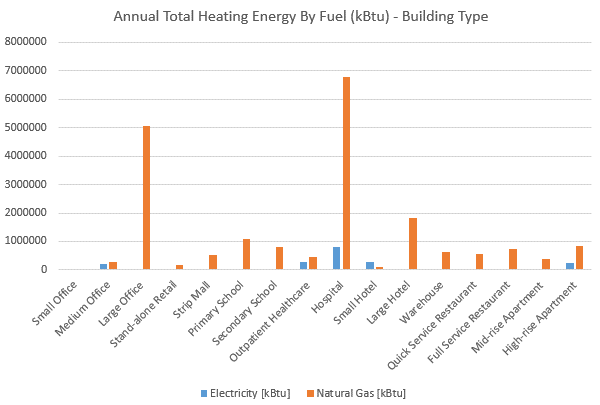
\includegraphics[width=0.7\linewidth]{heatFuel.png}
  \caption[Heating Fuel]{Heating Fuel}
  \label{fig:heatFuel}
\end{figure}
Electricity is the only fuel used for space cooling~\cite{DOE2015},
thus the EnergyPlus output parameter ``cooling:electricity'' is used
to represent space cooling demand. According to the suggested heat
rejection factor~\cite{Bhatia2015}, the heat recovery potential will
be calculated with $f = 1.15$ for Large Office and Hospital, and
$f = 1.25$ for the remaining building types:
\begin{equation}\label{eq:recover}
\text{Heat Recovery Potential} = \text{cooling:electricity} \times f
\end{equation}

In summary, to facilitate identification of energy recovery
opportunities for single buildings and within building groups, the
hourly ``heating:electricity'', ``heating:gas'' and
``cooling:electricity'' output will be extracted from energyPlus
simulation of DOE Commercial benchmark buildings.

\subsubsection{Input for Sizing District Co-generation
  System}
For the sizing of a district co-generation system, the relevant
information needed are the total heating demand, and the total
electricity demand. The general principle used in Lower Hill District
project ~\cite{baird2014} is to use the minimum total heat demand
(space heating and service hot water) over time to assess the minimum
capacity of electricity generation ($E_{heat}$) such that its heat
bi-product from electricity generation will always be consumed. The
maximum total electricity demand ($E_{elec}$) is used for assessing
the capacity of a backup system or a second phase system development
by $C_{backup} = E_{elec} - E_{heat}$ where $C_{backup}$ is the
capacity of electricity generation for the backup system or
second-phase development.

Heating demand assessed in the sizing of co-generation system is
different from the energy recovery use case in \sref{sec:inputRecover}
. It contains the space heating demand and the service hot water
demand. From the summary files of benchmark models, the fuel used for
providing service hot water is natural gas for all building types
(\tref{tab:hotWater})

The output parameter ``electricity:facility'' was extracted to
represent the total electricity demand.

\begin{table}[h!]
\centering
\caption{Service Hot Water by Fuel Type}
\label{tab:hotWater}
\begin{tabular}{l|l|l}
  \hline
                       &  Electricity {[}kBtu{]} & Gas {[}kBtu{]} \\
  \hline
  \hline
FullServiceRestaurant  & 0 & 253664.3       \\
Hospital               & 0 & 719402.7       \\
LargeHotel             & 0 & 6793934.2      \\
LargeOffice            & 0 & 231381.1       \\
MediumOffice           & 0 & 34178.3        \\
MidriseApartment       & 0 & 289719.3       \\
OutPatient             & 0 & 44054.5        \\
PrimarySchool          & 0 & 174768.0       \\
QuickServiceRestaurant & 0 & 82071.5        \\
SecondarySchool        & 0 & 441512.2       \\
SmallHotel             & 0 & 394017.1       \\
SmallOffice            & 0 & 10928.3        \\
Stand-aloneRetail      & 0 & 0.0            \\
StripMall              & 0 & 0.0            \\
SuperMarket            & 0 & 23799.7        \\
Warehouse              & 0 & 0.0            \\
  \hline
\end{tabular}
\end{table}

\pagebreak
\subsection{Simulation Data Analysis of the benchmark
  models}\label{boxPlot}
The output of EnergyPlus simulation of 16 benchmark buildings are
read, processed and plotted with a python program. The data loading
and processing utility is used in both data analysis and the dynamic
plot in the interface design.

The energy output retrieved from EnergyPlus include ``Heating:Gas'',
``Heating:Electricity'', ``Cooling:Electricity'', ``Water
Heater:WaterSystems:Gas'' and ``Electricity:Facility''. This section
will include some basic aggregated analysis of the data distribution.
The meaning of each output variable is listed in
\tref{tab:outputMeaning}:
\begin{table}[h!]
\centering
\caption{Table of EnergyPlus output and their meaning}
\label{tab:outputMeaning}
\begin{tabular}{l|l}
  \hline
EnergyPlus Output            & Meaning\\
  \hline
  \hline
Heating:Gas                  & Total gas for space heating         \\
Heating:Electricity          & Total electricity for space heating \\
Water Heater:WaterSystem:Gas & Total gas for service hot water     \\
Cooling:Electricity          & Total electricity for space cooling \\
Electricity:Facility         & Total electricity                  \\
  \hline
\end{tabular}
\end{table}

\subsubsection{Single Output}
By analysing the EnergyPlus ~\cite{EnergyPlus2015} simulation result
of the output above, we anticipate to gain a basic understanding of
the energy profile data distribution involved in the current
project. We would also want to use this as a basis to compare with the
additional analysis one can performed in a dynamic energy map in the
following sections.

To analyse general distribution of each output variable, we created a
box plot for each of the five variables. By analyzing each single
output, we discovered a great difference between different building
types. 

Hourly gas heating demand of the benchmark buildings range from 0 to
14000 kBtu. The majority (75\%) of all hourly consumption are below
2000 kBtu. All building types have a large amount of outliers above
the 75\% quartile. This indicates gas heating demand of all building
types are severely right skewed. Hospital has the highest median gas
heating demand of about 1100 kBtu. Outpatient Health Care has the
second larges hourly gas heating demand. In terms of peak demand,
Secondary School and Large Office have the highest peak hourly gas
heating demand (\fref{fig:HG}).
\begin{figure}[h!]
  \centering
  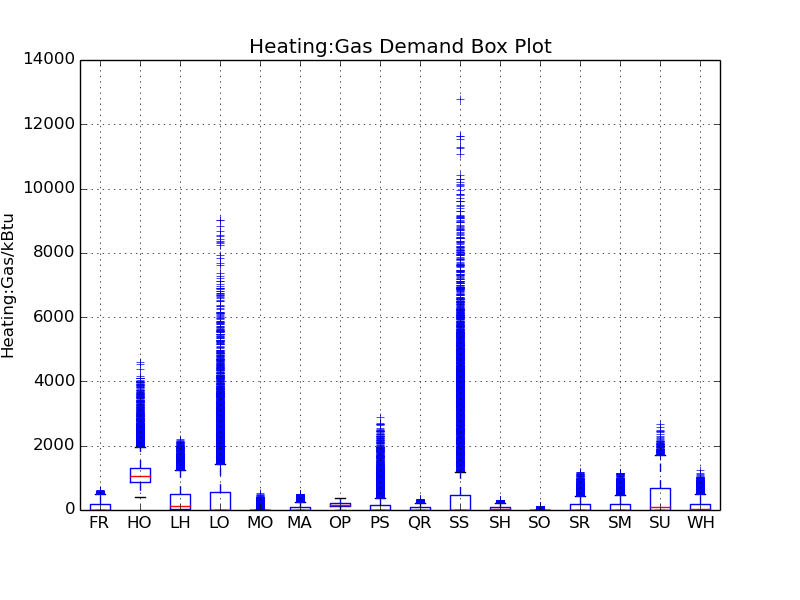
\includegraphics[width=0.7\linewidth]{HG}
  \caption[Heating:Gas Box Plot]{Heating:Gas Box Plot}
  \label{fig:HG}
\end{figure}%

Hourly hot water demand of the benchmark buildings range from 0 to
2500 kBtu, about 1/6 of the range of space heating gas demand. Most
buildings have median hot water hourly demand below 100 kBtu, except
that the median hot water demand of Large Hotel is around 700
kBtu. From \tref{tab:hotWater}, we can see that Stand-alone Retail,
Strip Mall and Warehouse has zero demand for service hot water. Large
Hotel also have a large amount of outliers above the 75\%
quartile. This indicates gas hot water demand of the Large Hotel is
severely right skewed. Hospital has the second largest median gas hot
water demand of about 100 kBtu. Large Hotel also stands out in peak
demand. (\fref{fig:WH}).
\begin{figure}[h!]
  \centering
  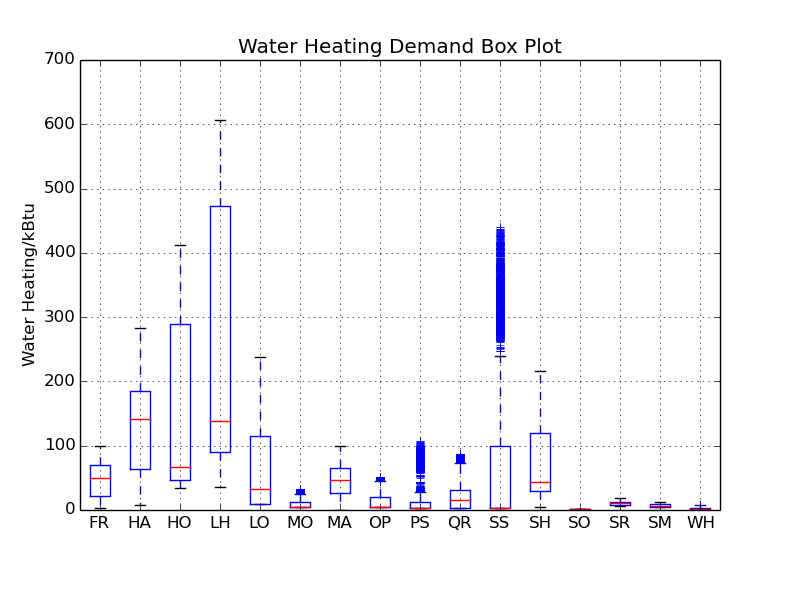
\includegraphics[width=0.7\linewidth]{WH}
  \caption[Water Heater:WaterSystem:Gas Box Plot]{Water
    Heater:WaterSystem:Gas Box Plot}
  \label{fig:WH}
\end{figure}%

From \tref{tab:heatFuel}, only Large Hotel, Medium Office, Midrise
Apartment, OutPatient Healthcare, Small Hotel and Stand-alone Retail
use electricity besides natural gas for space heating. Hourly
electricity heating demand of these buildings range from 0 to 1000
kBtu. All of them has nearly zero median electricity heating demand
and a large amount of outliers above (except for Midrise Apartment)
the 75\% quartile. This indicates electricity heating demand of all
the five building types are severely right skewed. Medium Office has
the highest hourly electricity heating peak demand and Outpatient
Healthcare has the second largest hourly electricity heating peak
demand (\fref{fig:HE}).

\begin{figure}[h!]
  \centering
  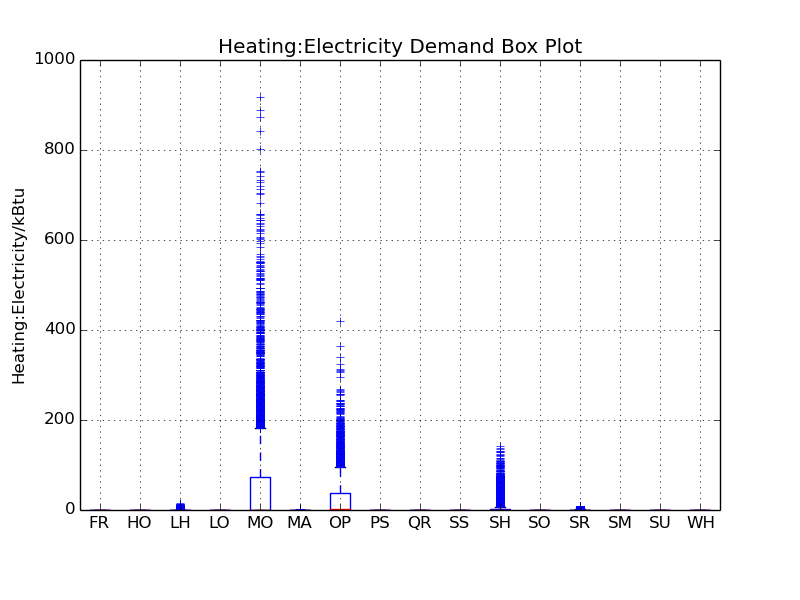
\includegraphics[width=0.7\linewidth]{HE}
  \caption[Heating:Electricity Box Plot]{Heating:Electricity Box Plot}
  \label{fig:HE}
\end{figure}% 

Hourly cooling demand benchmark building types range from 0 to 3000
kBtu, which is about 20\% of that of the peak gas heating demand. The
hospital has the largest median cooling demand of about 1500
kBtu. Large Hotel has the second largest median cooling demand. Both
Hospitals and Large Hotels do not have outliers, indicating their
hourly cooling demand distributions are less skewed. On the contrary,
all other building types have a large amount of outliers above the
75\% quartile, indicating a severe right skew for their hourly cooling
demand distribution. There are four building types with non-zero
median hourly cooling demand: Hospital, Large Hotel, Outpatient Health
Care and Small Hotel. This means they need space cooling for at least
50\% of the year. The constant cooling demand creates the
opportunities for energy recovery of cooling induced reject heat. The
building types with zero median hourly cooling demand then require
cooling only in the cooling season. In terms of hourly cooling peak
demand, the Secondary School has the highest peak demand of about
2700kBtu and Hospital has the second largest peak
demand(\fref{fig:CE}).
\begin{figure}[h!]
  \centering
  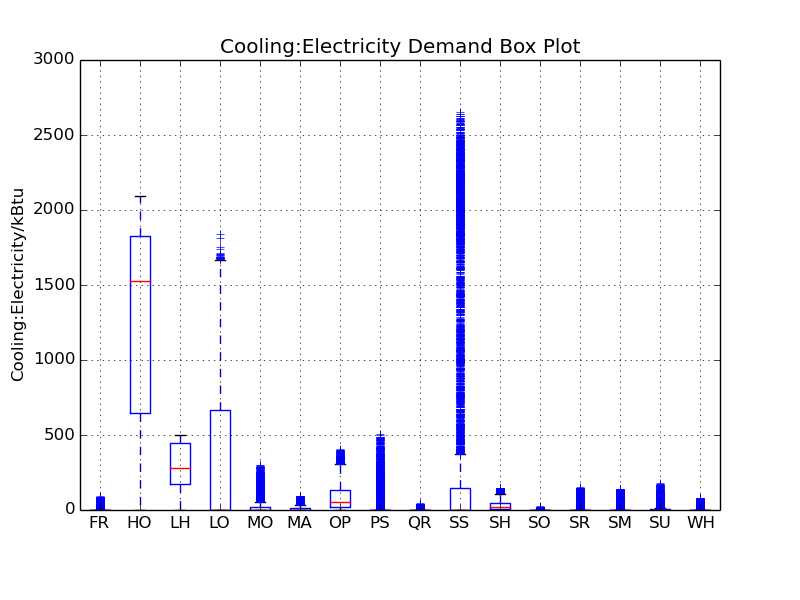
\includegraphics[width=0.7\linewidth]{CE}
  \caption[Cooling:Electricity Box Plot]{Cooling:Electricity Box Plot}
  \label{fig:CE}
\end{figure}%

The hourly electricity demand of benchmark buildings range from 0 to
6000 kBtu, which is about 40\% of that of the peak heating
demand. Comparing with other output variables, the electricity demand
distribution has less outliers in general. The Hospital has the
largest median hourly electricity demand (about 3400 kBtu). The Large
Office has the second largest median hourly electricity demand (about
1800 kBtu). Secondary School has the Largest electricity hourly peak
demand.

\begin{figure}[h!]
  \centering
  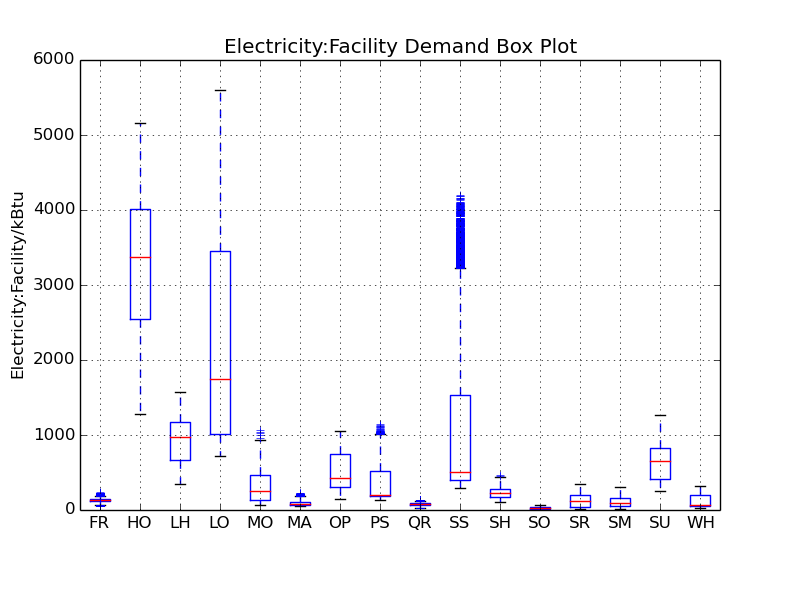
\includegraphics[width=0.7\linewidth]{EF}
  \caption[Electricity:Facility Box Plot]{Electricity:Facility Box
    Plot}
  \label{fig:EF}
\end{figure}%

\subsubsection{Space Heating Demand vs. Space Cooling Demand}
Hourly space heating demand of the benchmark buildings mainly closely
follows the distribution of gas heating demand, with minor demand
increase in Medium Office and Outpatient Health Care (\fref{fig:SH}).

\begin{figure}[h!]
  \centering
  \begin{subfigure}{0.4\textwidth}
  \centering
  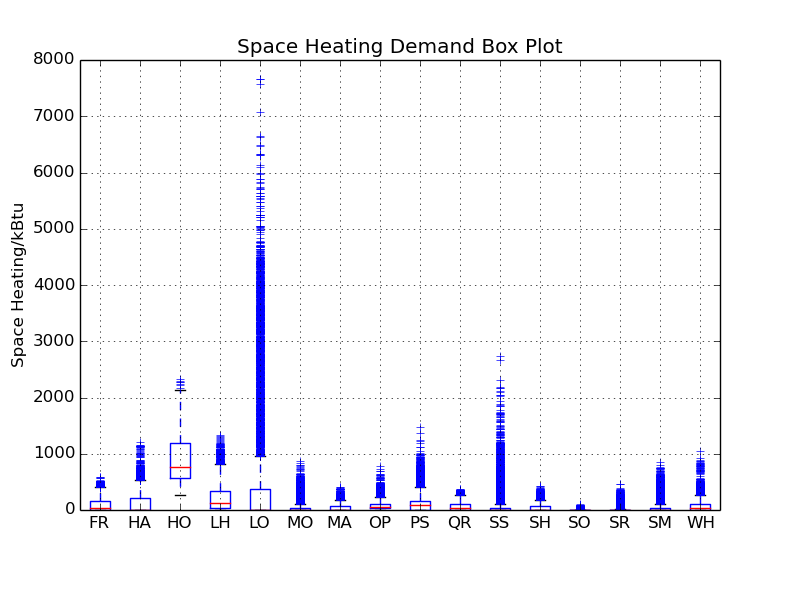
\includegraphics[width=\linewidth]{SH}
  \caption[Space Heating Demand Box Plot]{Space Heating Demand Box
    Plot}
  \label{fig:SH}
\end{subfigure}
~
\begin{subfigure}{0.4\textwidth}
  \centering
  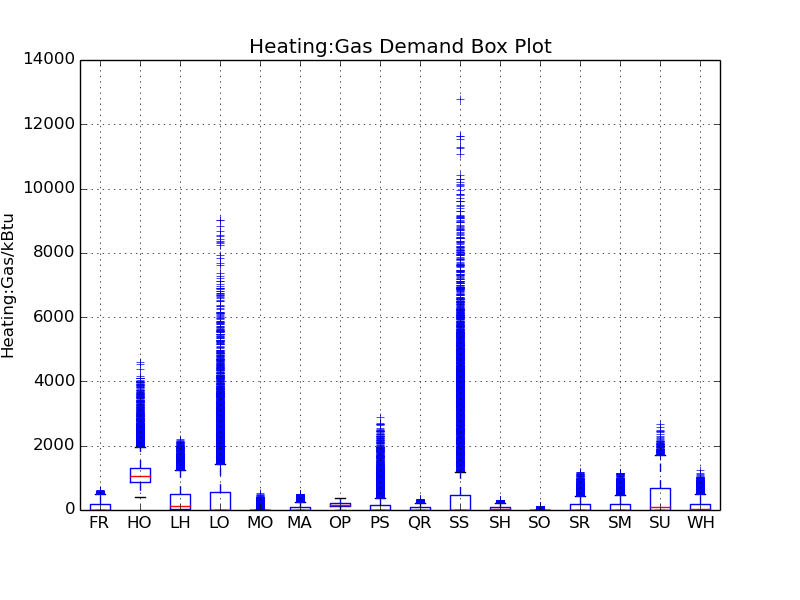
\includegraphics[width=\linewidth]{HG}
  \caption[Heating:Gas Box Plot]{Heating:Gas Box Plot}
  \label{fig:HG2}
\end{subfigure}
\caption[Comparing Heating:Gas and Space Heating]{Comparing
  Heating:Gas and Space Heating}
\end{figure}

Comparing the space heating (Heating:Gas and Heating:Electricity) with
space cooling (Cooling:Electricity), we can see that the heating peak
demand is larger than cooling peak demand for all building types. The
Hospital, Large Hotel and Outpatient Health Care have both the highest
median space heating and cooling demand, indicating a potential for
single building level energy recovery.
\begin{figure}[h!]
  \centering
  \begin{subfigure}{0.4\textwidth}
  \centering
  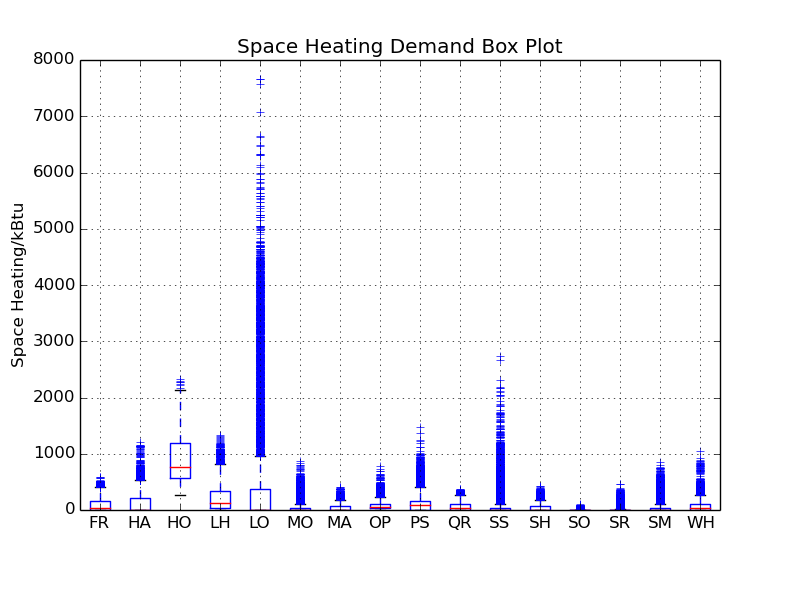
\includegraphics[width=\linewidth]{SH}
  \caption[Space Heating Demand Box Plot]{Space Heating Demand Box
    Plot}
  \label{fig:SH}
\end{subfigure}
~
\begin{subfigure}{0.4\textwidth}
  \centering
  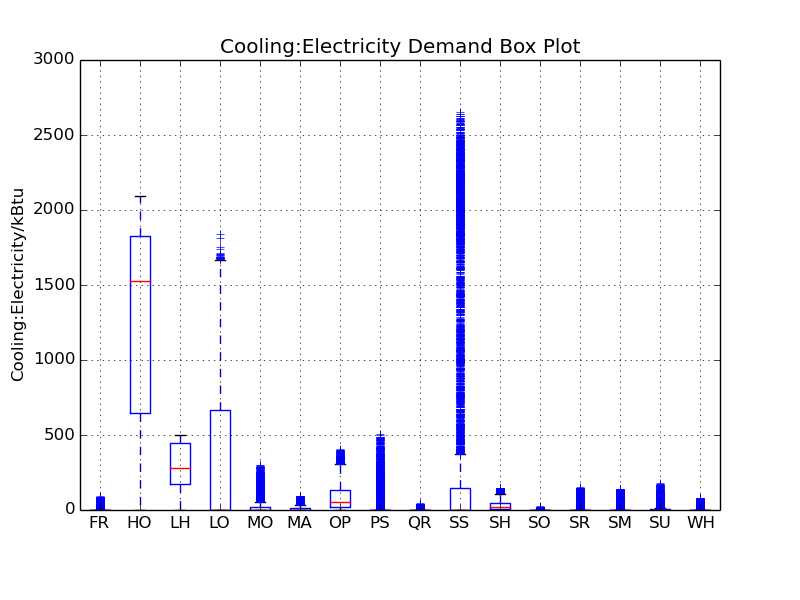
\includegraphics[width=\linewidth]{CE}
  \caption[Cooling:Electricity Box Plot]{Cooling:Electricity Box Plot}
  \label{fig:CE2}
\end{subfigure}
\caption[Comparing Space Heating and Space Cooling Demand]{Comparing
  Space Heating and Space Cooling Demand}
\end{figure}

\subsubsection{Heating Demand vs. Electricity Demand}
Comparing the heat and power demand of each benchmark building type
with the ``heat to power ratio''(HTPR), one of the important
parameters of a CHP plant. Depending on the prime mover types, a CHP
plant can produce 0.6 to 10 unit of waste heat for one unit of
electricity generation~\cite{introCHP2010}. From \fref{fig:HTPR}, we
can see the range of HTPR is from 0 to 25 and the median of HTPR are
all below 1. The building types with a high median HTPR include Large
Hotel, Midrise Appartment, Outpatient Health Care and First Service
Restaurant. Increase the number of buildings with high HTPR ratio is
helpful in more fully reuse of the waste heat from power
generation. In addiction, the large range of Heat to Power ratio also
indicates the necessity of heat storage equipment.
\begin{figure}[h!]
  \centering
  \begin{subfigure}{0.4\textwidth}
  \centering
  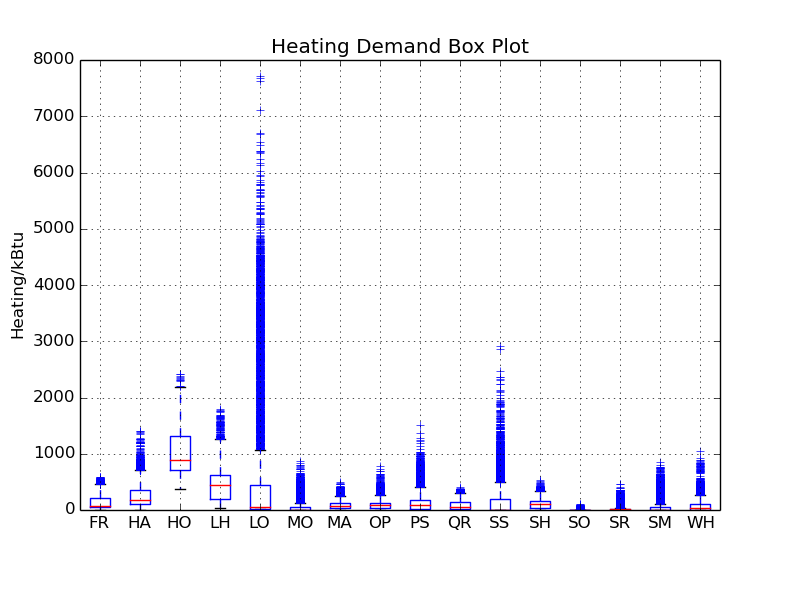
\includegraphics[width=\linewidth]{H}
  \caption[Heating Demand Box Plot]{Heating Demand Box
    Plot}
  \label{fig:H}
\end{subfigure}
~
\begin{subfigure}{0.4\textwidth}
  \centering
  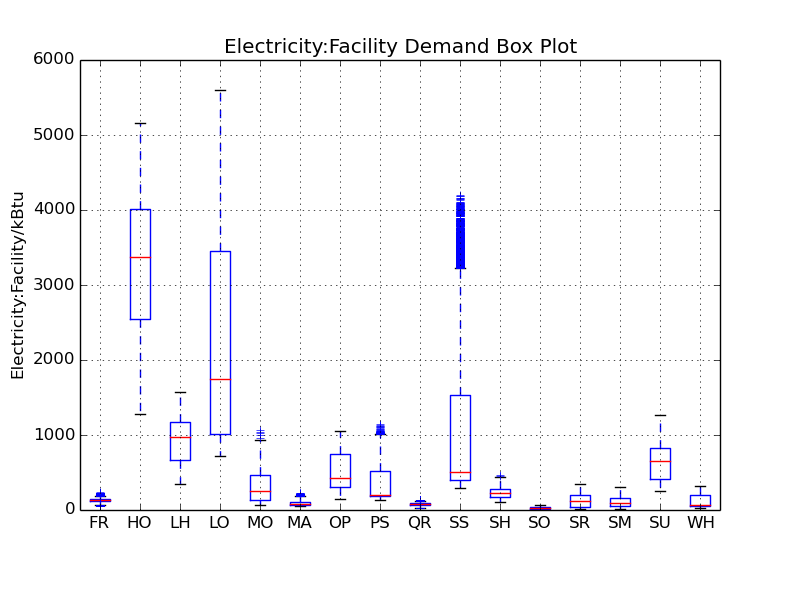
\includegraphics[width=\linewidth]{EF}
  \caption[Electricity Demand Box Plot]{Electricity Demand Box Plot}
  \label{fig:EF2}
\end{subfigure}
\caption[Comparing Heating and Electricity Demand]{Comparing Heating
  and Electricity Demand}
\end{figure}

\begin{figure}[h!]
  \centering
  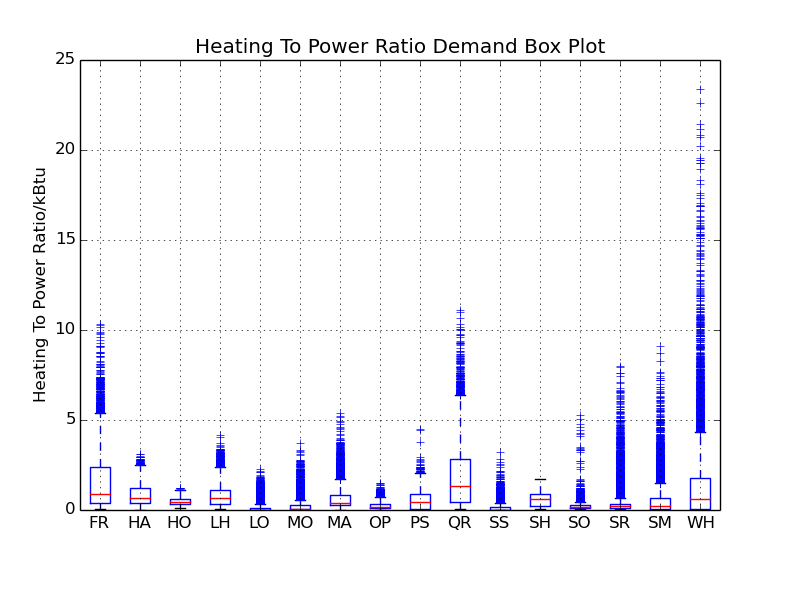
\includegraphics[width=0.7\linewidth]{HTPR}
  \caption[Heat to Power Ratio Box Plot]{Heat to Power Ratio Box Plot}
  \label{fig:HTPR}
\end{figure}%

\pagebreak
\subsection{3D GIS Model Geometry}
The conceptual community model is constructed in
CityEngine~\cite{cityEngine2015}. CityEngine is a software developed
by Esri~\cite{Esri2015}. It can aggregate geographic information into
buildings and is capable of smoothly transition models to
ArcGIS\cite{ArcGIS2015}, one of the widely applied tools for
Geo-referenced data presentation and analysis. Buildings in CityEngine
is defined with ``rules'' using CGA (Computer Generated Architecture)
shape grammar that is unique to CityEngine. The rule-based modeling of
urban environment enables fast construction and easy adjustability of
urban density, skyline and terrain control. It also enables easy
aggregation of Energy profile data into 3D urban environment models,
which is difficult to do in the current ArcGIS, the technical details
will be explained in \aref{AppendixA}.

Although the urban environment in this study is a conceptual setting,
we still want it to reflect the topological and density pattern in a
real urban environment. To construct the model, we first extracted the
topological pattern from an existing urban design project, the Mellon
Arena Project~\cite{baird2014} (\fref{fig:mellonArena}.  There are
eight building types in the project: Residential (43\%), Town House
(2.9\%), Community Center (0.4\%), Commercial (3.8\%), Office (19\%),
Hotel (4.7\%), Cinema (1.4\%) and Garage (24.7\%).

\begin{figure}[h!]
  \centering
  \begin{subfigure}{0.5\textwidth}
  \centering
  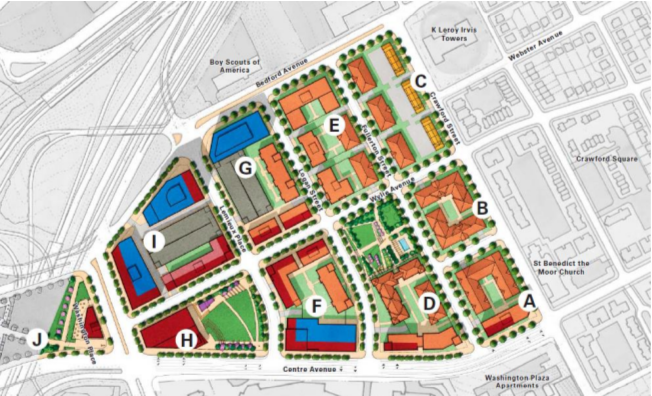
\includegraphics[width=\linewidth]{mellonArena}
  \caption[Mellon Arena Site Plan]{Mellon Arena Project Site Plan View}
  \label{fig:mellonArena}
\end{subfigure}
~
\begin{subfigure}{0.3\textwidth}
  \centering
  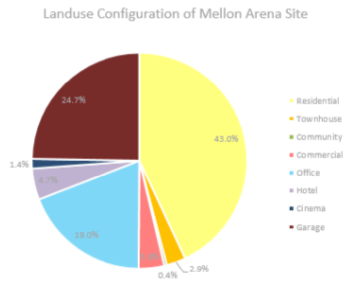
\includegraphics[width=\linewidth]{mellonPie}
  \caption[Mellon Arena Site Land Use]{Mellon Arena Site Land use Configuration}
  \label{fig:mellonPie}
\end{subfigure}
\end{figure}
The 16 building types in DOE commercial benchmark models do not
perfectly correspond to those in the Mellon Arena Site. In order to
adapt the topological pattern of the Mellon Arena Project, a mapping
(function) from building types of Mellon Arena Site to building types
of DOE models is created as is shown in \tref{tab:typeMap}.
\begin{table}[h!]
  \centering
  \begin{tabular}{c| c| c}
    \hline
    Mellon Arena Type &Probability &DOE Building Type\\
    \hline
    \hline
    Hotel &50\%&Large Hotel\\
    \cline{2-3}
    &50\%&Small Hotel\\
    \hline
    Office &30\%&Large Office\\
    \cline{2-3}
    &30\%&Medium Office\\
    \cline{2-3}
    &30\%&Small Office\\
    \hline
    Residential &100\%&Midrise Appartment\\
    \cline{1-2}
    Townhouse &100\%&\\
    \hline
    Commercial &25\%&Full Service Restaurant\\
    \cline{2-3}
    $+$ Cinema $+$&25\%&Quick Service Restaurant\\
    \cline{2-3}
    Community &25\%&Super Market\\
    \cline{2-3}
    Center &25\%&Stand-alone Retail\\
    \hline
  \end{tabular}
  \caption{Mapping of Mellon Arena to Building Types of DOE benchmark model}
  \label{tab:typeMap}
\end{table}

The four major building sectors involved in the current project are
residential, commercial, office and hotel. Their topological pattern
is represented in Figure \ref{fig:mellonTop}. The conceptual model
construction follows the building type topological pattern and the
urban density as the Lower Hill District Project (\fref{fig:sitePlan})

After the land use is assigned (\fref{fig:sitePlan}), one rule file is
applied to all the building lots and generates building geometries by
extruding the building lot (with an offset to the interior) according
to the number of floors of the benchmark buildings. We intend to make
the building geometry simple in order to highlight the color of each
building that encodes its energy demand.

\begin{figure}[h!]
  \centering
  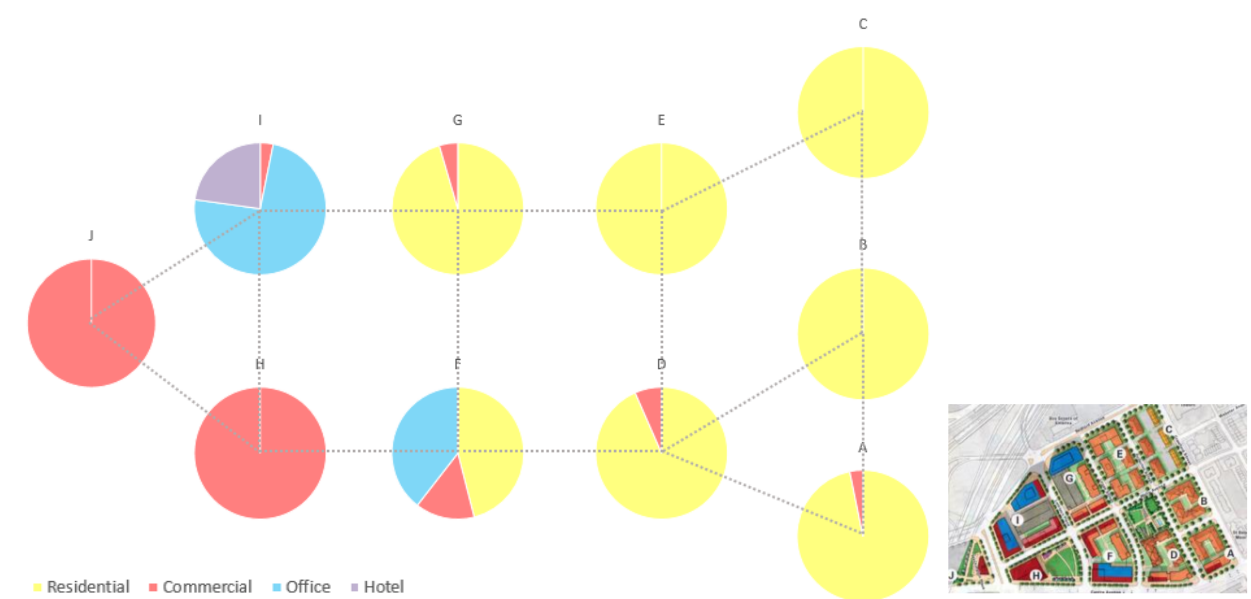
\includegraphics[width=\linewidth]{mellonTop}
  \caption[Building Type Topology]{Building Type Topological Pattern, Mellon Arena}
  \label{fig:mellonTop}
\end{figure}

\begin{figure}[h!]
  \centering
  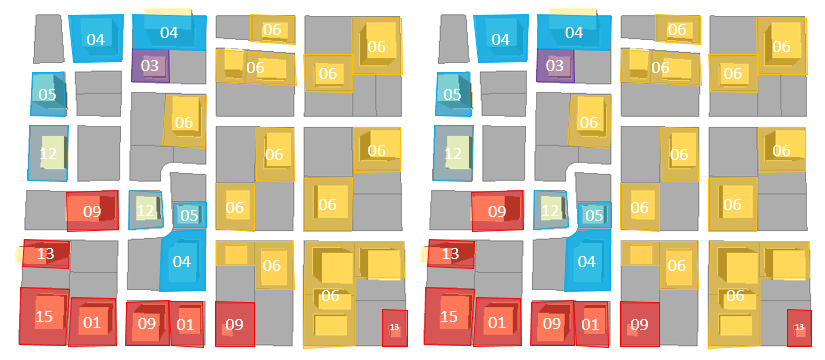
\includegraphics[width=\linewidth]{sitePlan}
  \caption[Conceptual Model Site Plan]{Site Plan of Conceptual Model}~ (01: Full Service
  Restaurant, 03: Large Hotel, 04: Large Office, 05: Medium Office,
  \\06: Midrise Apartment, 09: Quick Service Restaurant, 12: Small
  Office, \\13: Stand-alone Retail, 15: Super Market)
  \label{fig:sitePlan}
\end{figure}

\subsection{Aggregating Hourly Energy Data to 3D GIS Model}\label{sec:aggregateTime}
The authors have experimented with two approaches to aggregate energy
profile data into the conceptual model constructed in CityEngine
\begin{enumerate}[1)]
\item Importing 3D models from CityEngine to ArcScene and aggregate
  the energy data (in the form of a table) into the 3D feature with
  ``one-to-many'' join. For more details please refer to Appendix X

\item Write the energy profile data directly in the rule file for
  building generation in CityEngine. For more details please refer to
  \aref{AppendixA}

\item Process the color encoding outside of CityEngine and write the
  generated color encoding representations in CityEngine
\end{enumerate}

The second approach has the advantage of 1) ready-to-use data
classification method and map symbol templates that facilitates
choropleth map design 2) the ``time-slider'' function for creating a
time-wise navigation and animated map. \fref{fig:arcgisTime} shows the
interface slider and the dynamic map of heating energy demand for the
conceptual model using ArcGIS. There are several problems of this
approach: 1) its high requirement of computational power makes it
infeasible to model or view on a typical PC. The authors only
succeeded in importing the hourly energy profile data when using point
features to represent building geometry. Even for the relatively
simple 3D models in the current study, a relatively higher performance
machine (Dell Precision T1600 Quad Core Intel Xeon, 3.10GHz RAM - 16GB
was used) was used in importing the data, the authors only suceeded in
importing one month of data, never for one year. This technical issue
makes it impossible to using the current ArcGIS platform to implement
high temporal resolution dynamic maps without either truncating time
range or reducing the complexity for building geometry
representation. 2) The time dimension only exist inside the map
file. This means even one produced a dynamic energy map, one cannot
share it without packing all related files and send to others. This
requires the viewer end to have the same high performance
computer. Although the animated map can be exported, the output
animation contains neither any form of temporal label nor the control
of playback. Without time legend, when and for how long the dynamic
changes happen are not shown. 3) For 3D GIS model, it does not contain
a proper function to extract single frames of map images, making it
impossible to implement exterior interface that deals with 3D maps
images.

The first approach, on the contrary, provides more flexibility but
also requires much user-end work including: pre-processing of energy
profile data, implementing data classification method and the
bivariate color ramp. An interface is also needed for visualising the
image sequence.

\begin{figure}[h!]
  \centering
  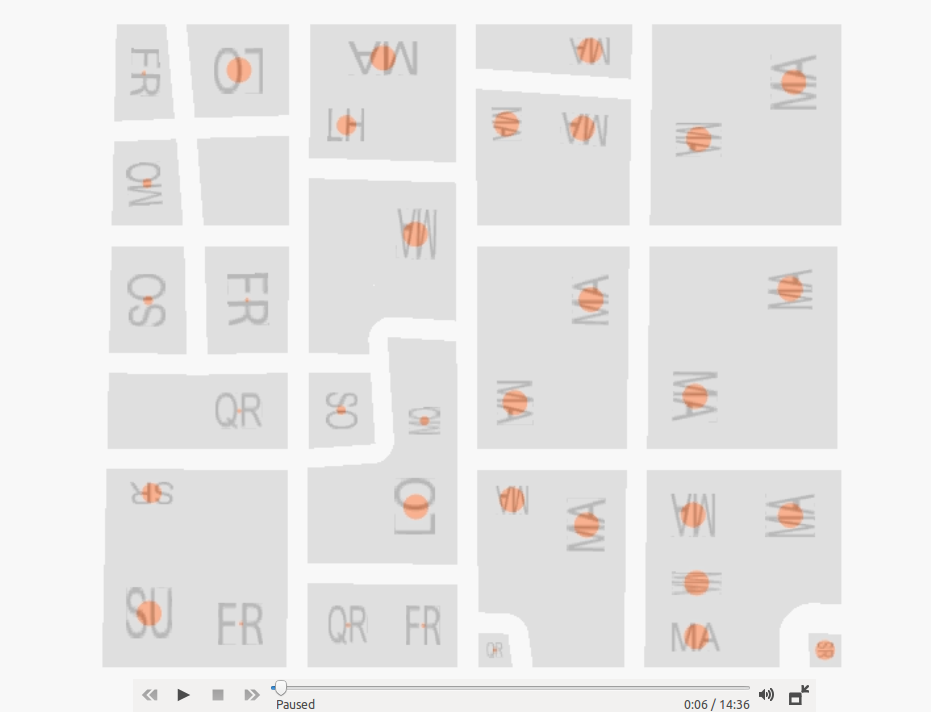
\includegraphics[width=0.5\linewidth]{arcgisTime}
  \caption{ArcGIS Time Slider for Temperal Data Display}
  \label{fig:arcgisTime}
\end{figure}

Due to limited time, the experimented GIS software are only restricted
to ArcGIS and CityEngine. There could be better alternatives to
achieve a dynamic map with more elegance. Find a better alternative
software to implement a dynamic map could be part of the work of the
next stage of the project.

\chapter{Interface Design} % Main chapter title

\label{Chapter6} % For referencing the chapter elsewhere, use \ref{Chapter1} 

\lhead{Chapter 6. \emph{Interface Design}} % This is for the header on each page - perhaps a shortened title

%----------------------------------------------------------------------------------------
This section provides detailed illustration of the non-interactive
(map animation) and interactive dynamic energy map implementation and
design choices regarding the interactive dynamic energy map. The
section starts with a general overview that explains possible
approaches to add the time dimension in an energy map. Then the
non-interactive energy map (map animation) approach is presented. For
the non-interactive animation, the advantages and disadvantages
between different symbol or color representation on the effectiveness
of conveying information was briefly discussed.

Next a detailed documentation of the dynamic energy map interface is
presented. The layout and functions of each components of the
interface is explained and the design of each component based on
literature studies of dynamic map design is discussed. The use of
dynamic energy map to identify energy recovery opportunities and to
help design and size a district energy system is demonstrated.

\section{Overview}

Dorling and Openshaw pointed out that a dynamic map provides new
potential and possibilities for data analysis but also poses a great
challenge as a result of the less developed theory in space-time
pattern detection and measurement~\cite{Dorling1992}. In order to
better conduct a space-time visualization of the space-time energy
demand information in the dynamic energy map,literature studies on
space-time map visualization were used to design the dynamic energy
map.

Brownrigg mentions several methods of representing time on a map: 1) a
graph or chart that represents a function over time or a time line for
displaying chronological events 2) a sequence of snapshots displayed
over time (animated map) 3) small-multiples of snapshots of changing
states ~\cite{Brownrigg2005}.

Based on the classification above, method 1) and 2) were applied to
represent time for the dynamic energy map. The dynamic plot of
temporal time series uses method 1) to anchor the quantitative
information. The sequential map image display is using method 2). The
researcher did not use the small multiple method (method 3)). The
choice is based on the following points mentioned by Brownrigg: 1) the
number of snapshots in one display is limited and the finer the detail
per snapshot, the less snapshots one can contain in one display. Since
the 3D representation is chosen as one of the major map display
methods (2D map is also available), the level of details per image is
relatively high. This will result in a very small number of multiples
per display~\cite{Brownrigg2005} 2) the subtle changes are easier to
be noticed in the form of animation than with small-multiples
~\cite{Brownrigg2005}. Both drawbacks of small-multiple method will
impair the ability to convey the rapid temporal changes of community
energy behavior, hence is not suitable for the current project.

\section{(Non-interactive) Map Animation} \label{anime} 

Map animation was introduced to cartography in
1930s~\cite{Harrower2008}. Its major application include: 1)
demonstrating the dynamic process of geographic events (weather maps
in weather forecasting is such an example) 2) assisting pattern
recognition and knowledge development for scientific researches. The
study by Dorling and Openshaw is an example of application 2), where
they discovered new leukaemia hotspots through animated
maps~\cite{Dorling1992}.  Animated maps are proven to be more powerful
in conveying the spatial-temporal pattern than static
maps~\cite{McEachern1998}.

The level of user control of playback behavior of animated maps is
debatable. Providing the full freedom of adjusting the playback can
enhance pattern understanding~\cite{Nelson1998}, but it might also
reduce time animation to still images and impair its ability in
conveying temporal changes ~\cite{Lowe2004}. In the current dynamic
map project. The researcher observed that the non-interactive map
animation is especially helpful in conveying the dynamic energy
changing and the non-coincident peak arriving time of different
buildings in the community. Resch et al.\ suggest that the interface
for general public should ``ensure that the amount of information
shown to the users at any given time, and its complexity, are
reduced''~\cite{Resch2014}. The non-interactive animated map could be
one of the potential choices for an interface of a dynamic energy map
with general public as the target user group.

For this project a continuous color encoding method was used in the
creation of non-interactive animation of a univariate gas heating
energy demand map. Similar to the National Heat Map, the Calgary Map
and the EMIOFN project (\tref{tab:mapRep}) discussed in
\sref{sec:mapRepre}, a red to blue color ramp is used in the map
display. Different from the cases above, the current project chose to
represent high heat demand with blue and low heat demand with red as a
result of a limited survey of potential users. Each color within this
red-to-blue color scheme is represented as a real number between 0 and
1 with 0 representing pure red and 1 representing pure blue.

The first approach to calculate the corresponding color for each
heating energy value is to calculate the normalized distance between
the current value and the maximum value (\eref{eq:linear}).

\begin{equation}\label{eq:linear}
  {E(t) – E_{max} \over E_{max}}
\end{equation}

$E(t)$ is the energy consumption for the current time spot $t$,
$E_{max}$ is the maximum energy consumption over the year. The problem
for this approach is that the color changing is not visible enough as
a result of a extremely right skewed energy data (with each data point
representing the hourly energy consumption of a certain building in
the community at a certain hour of a year) distribution
(\fref{fig:heatOri}).

\begin{figure}[h!]
  \centering
  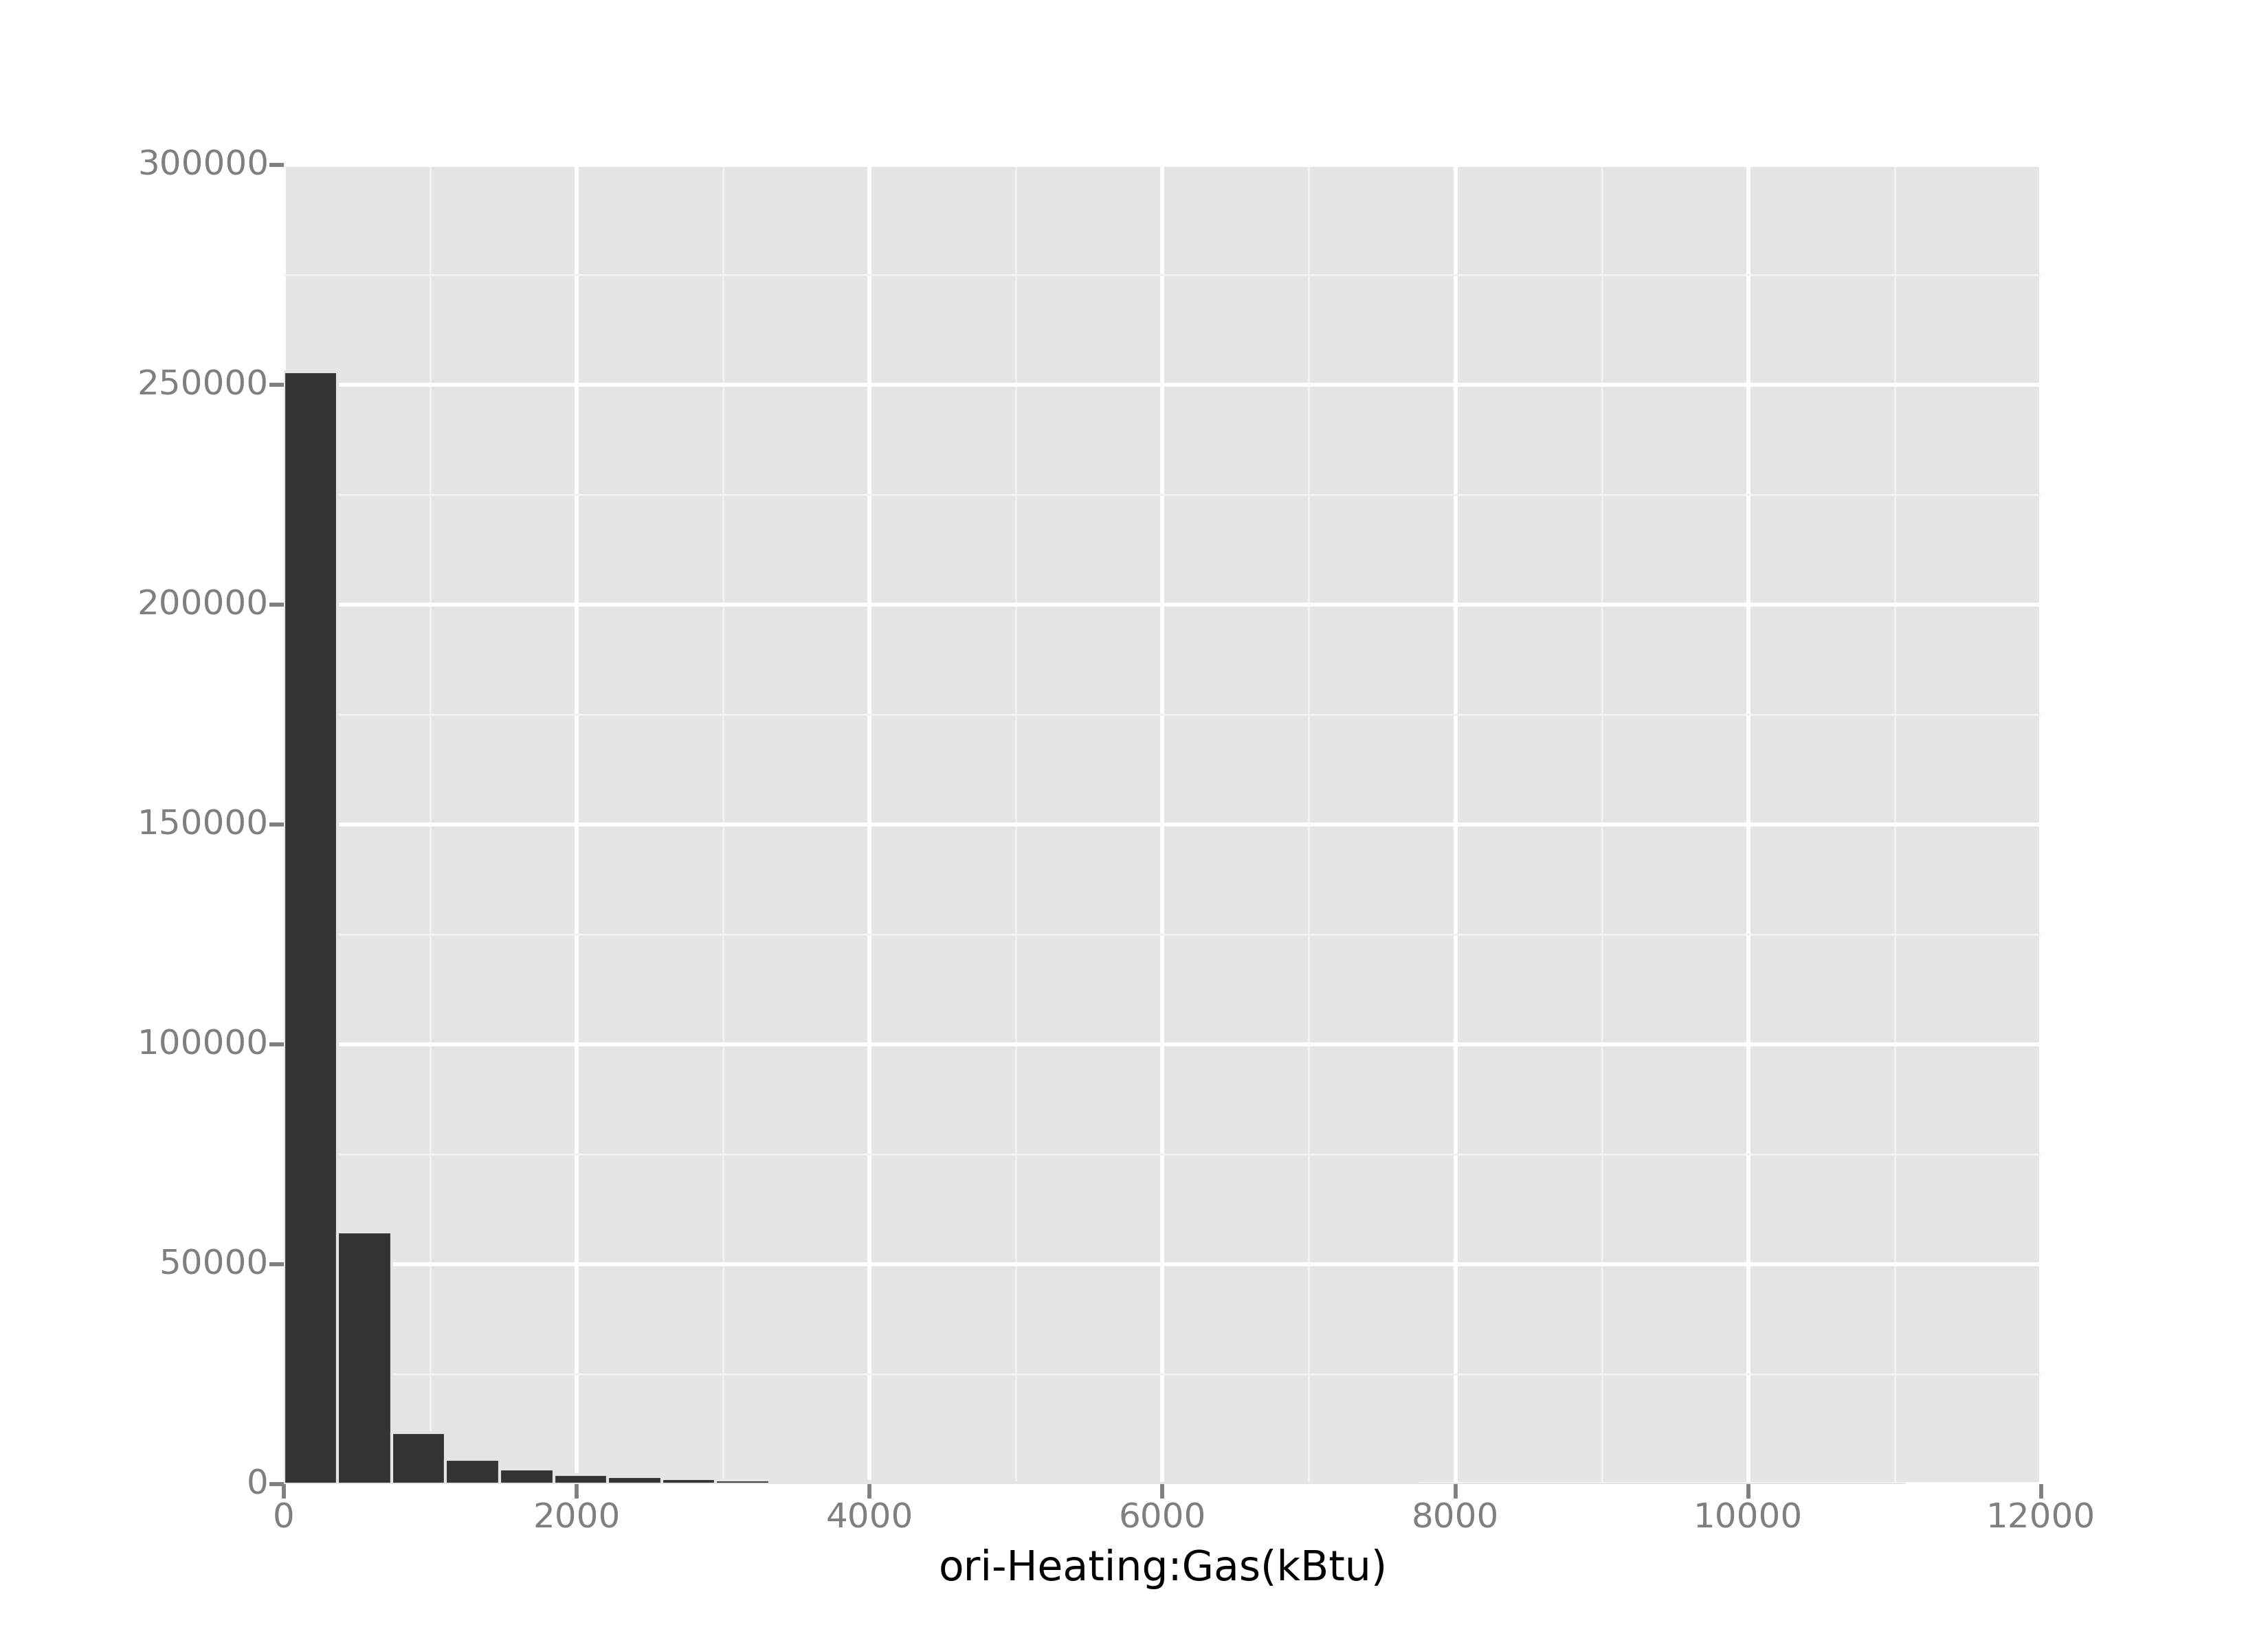
\includegraphics[width=0.7\linewidth]{heatOri.png}
  \caption[Heating Demand Histogram of Conceptual City]{A histogram of
    hourly energy consumption per building, for the 68 buildings in
    the community}
  \label{fig:heatOri}
\end{figure}

By directly applying this normalized color scheme, the color
distribution on a map will be very un-even, with most of the buildings
colored with the red color for most of the time.

Kolter and Ferreira discovered that the annual total energy
consumption of the 6500 buildings in Cambridge MA area follows a
``log-normal'' distribution~\cite{Zico2011}. By applying similar log
scaling for the hourly heating energy data of the community, the researcher found
that the hourly heating energy distribution also roughly follows a
normal distribution (\fref{fig:heatLog}). the researcher apply log scaling to
flatten the distribution and calculate the color from energy
($E(t)$) as follows:

\begin{equation}\label{eq:log}
  {\ln(E(t)) – \ln(E_{max}) \over \ln(E_{max})}
\end{equation}

\begin{figure}[h!]
  \centering
  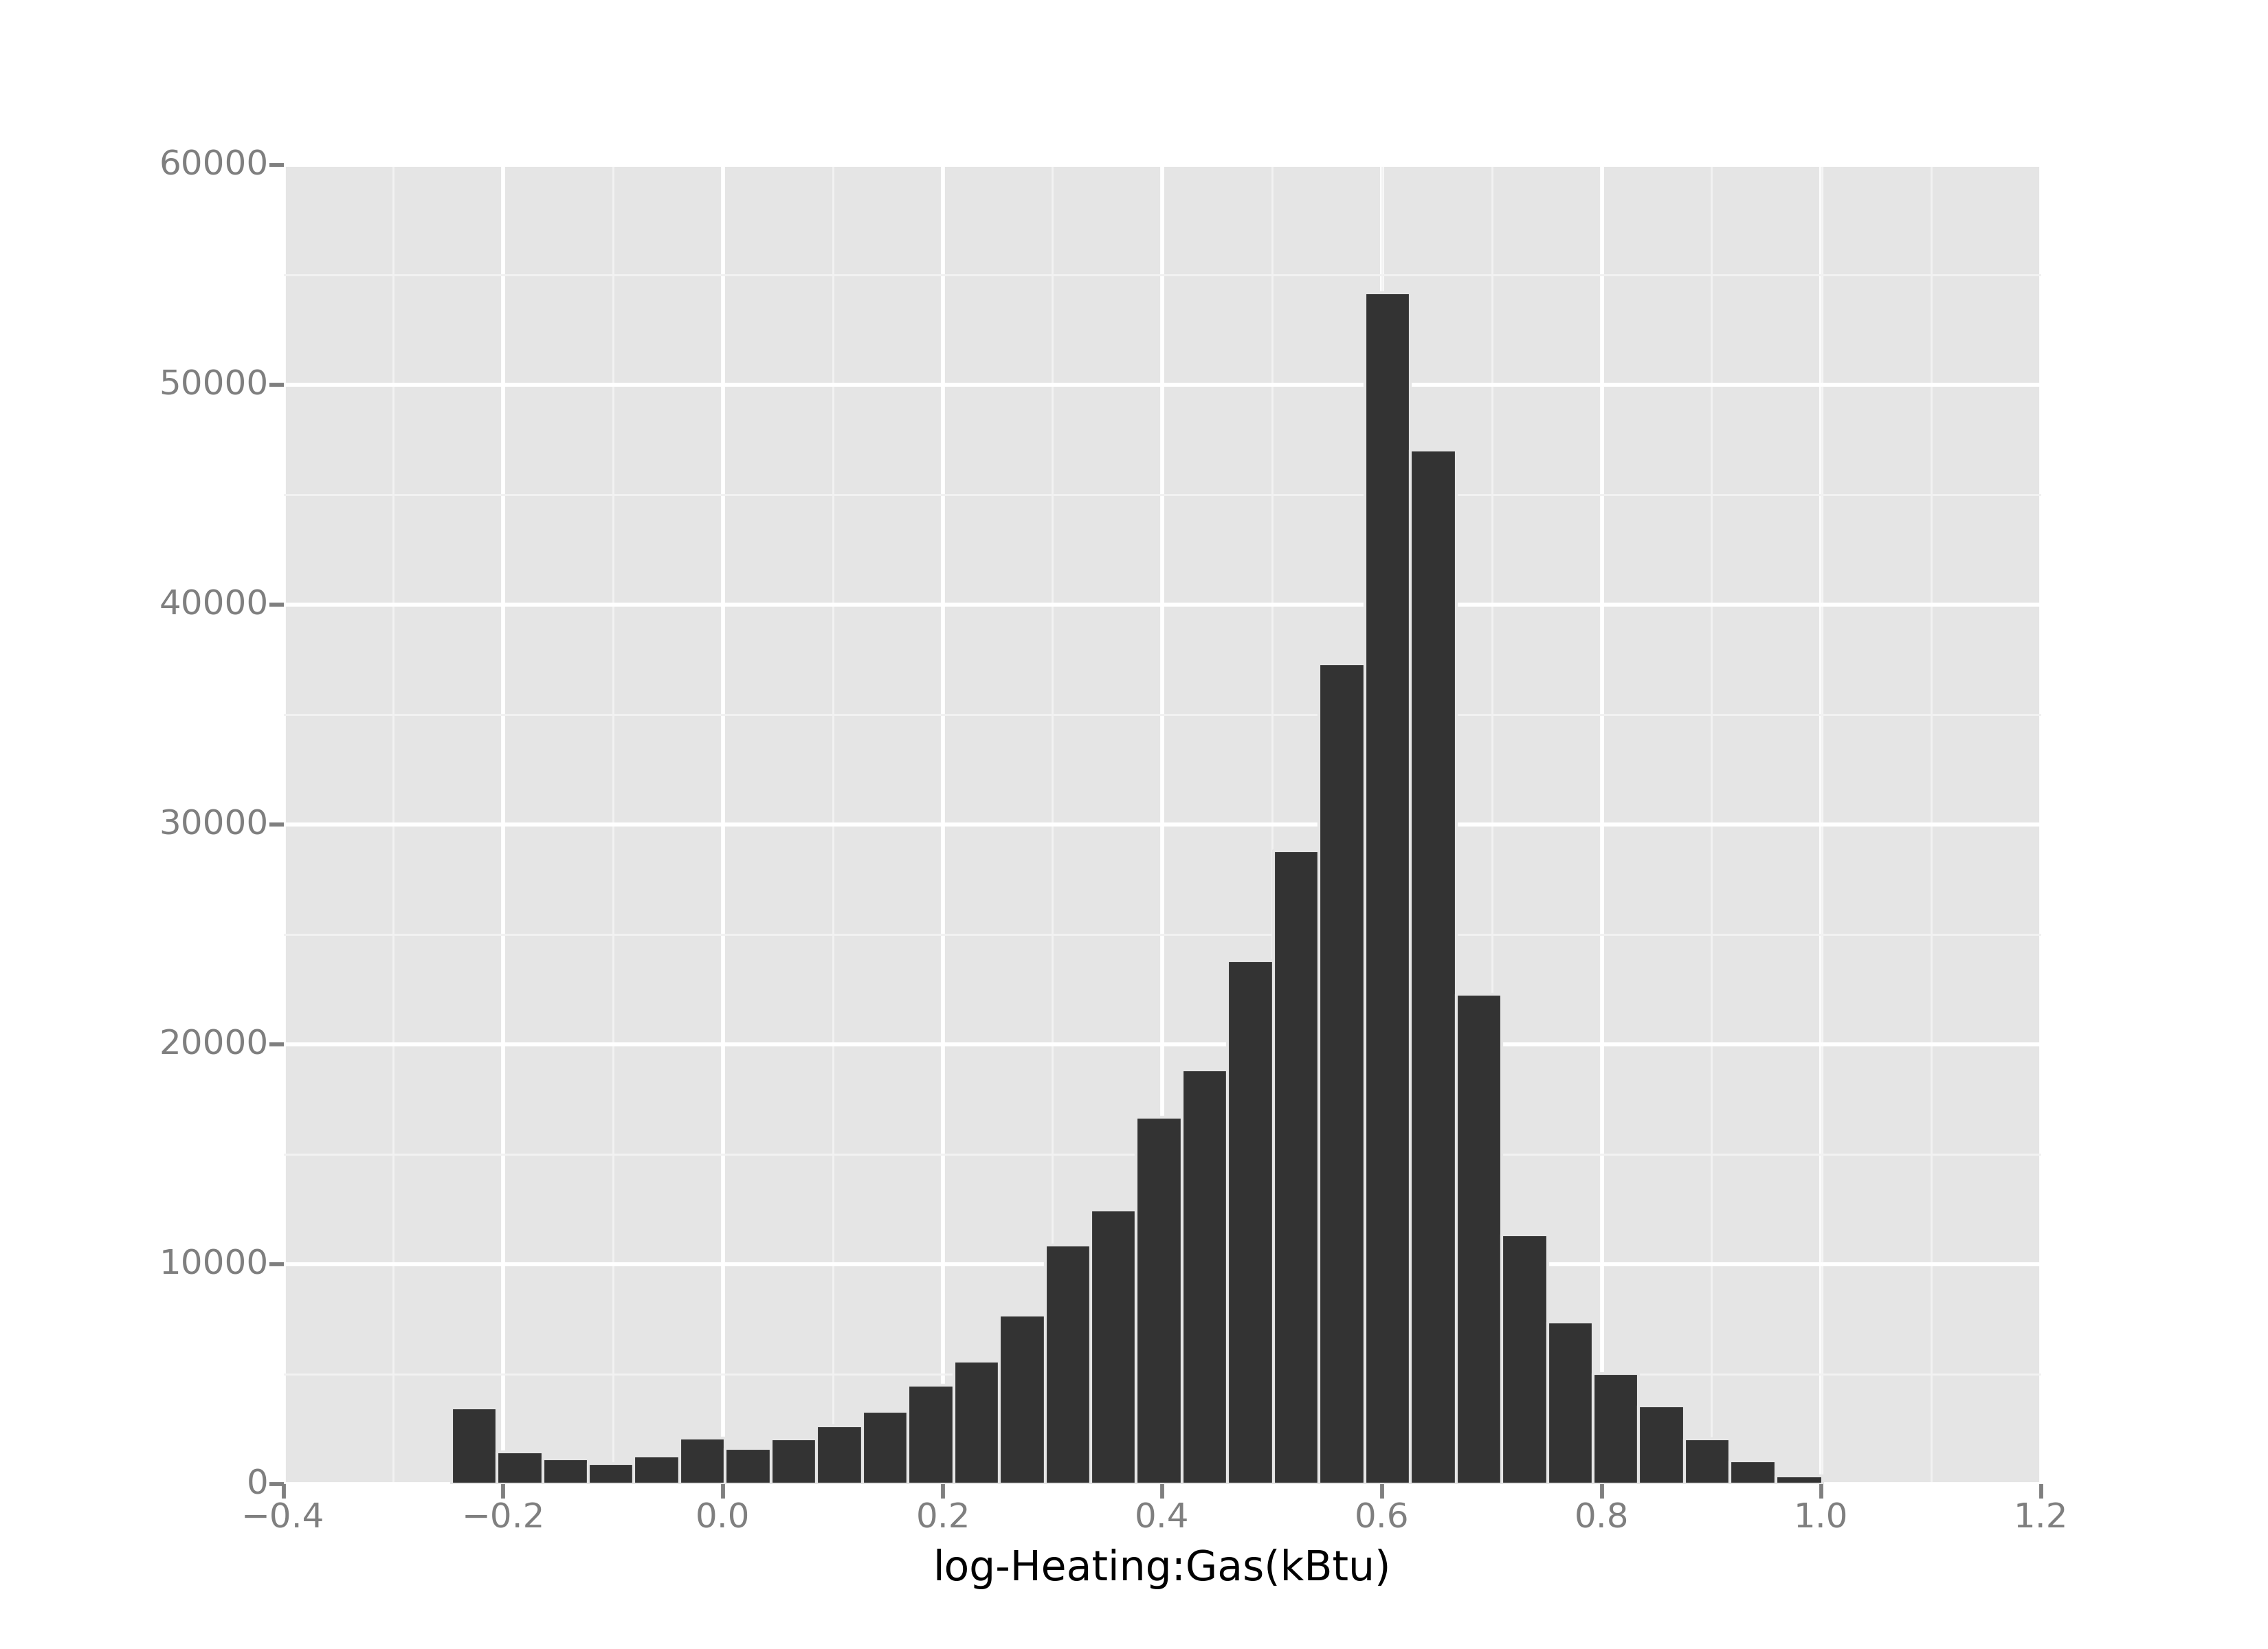
\includegraphics[width=0.7\linewidth]{heatLog.png}
  \caption[Heating Demand of Conceptual City]{Heating Demand of
    Conceptual City}
  \label{fig:heatLog}
\end{figure}

\fref{fig:img0002} is one snapshot of the conceptual urban environment
model under the log scaled calculation method in \eref{eq:log}.
\begin{figure}[h!]
  \centering
  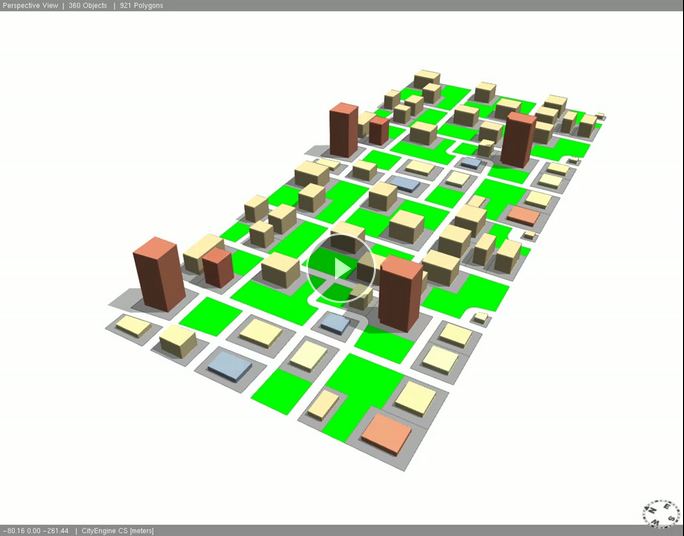
\includegraphics[width=0.7\linewidth]{img0002.png}
  \caption[Animation Demo of the Color Calculation]{Animated
    demonstration of the log-scaled dynamic energy heating demand map}
  \label{fig:img0002}
  \href{http://www.armechxyj.com/energy-mapping.html/#colorAnime}{Click
    here to go to the animation link}.
\end{figure}

In the dynamic energy map interface design, the researcher applied a
discrete color encoding with a seven-class bivariate choropleth
representation (\tref{tab:breakpoint}). The break points are
calculated purely with the Quantile method in
\sref{dataClassification}. This allows for a quantitative legend that
can depict more specific energy demand information. An animation with
this discrete color scheme is also created and can be viewed and
downloaded
\href{http://www.armechxyj.com/energy-mapping.html#redblueAnime3d}{through
  this link}.

\begin{table}[]
\centering
\caption{Heating-Cooling Breakpoints in the Interface}
\label{tab:breakpoint}
\begin{tabular}{rr|rr}
  \hline
heating &      & cooling &     \\
  \hline
  \hline
kBtu    & Ton  & kBtu    & Ton \\
5       & 60   & 2       & 24  \\
22      & 264  & 7       & 84  \\
50      & 600  & 15      & 180 \\
91      & 1092 & 26      & 312 \\
136     & 1632 & 56      & 672 \\
213     & 2556 & 72      & 864\\
  \hline
\end{tabular}
\end{table}

Although the initial conditions of the map instances using the
continuous and discrete encoding method are different: the animation
with continuous color encoding depicts only one variable (gas heating)
while the animation with discrete color encoding depicts two variables
(space heating and cooling), the researcher observed that the
continuous color encoding method seems to be better in demonstrating
the general pattern of energy changing behavior. Further evaluations
are needed to compare these two approaches and justify the design
choice of a discrete or continuous color scheme.
\section{Interactive Dynamic Map Interface}
\subsection{General Layout}
The general layout of the dynamic map interface is displayed in
\fref{fig:interfaceLayout}. It contains the following major sections :
\begin{figure}[h!]
  \centering
  \begin{subfigure}{0.7\textwidth}
  \centering
  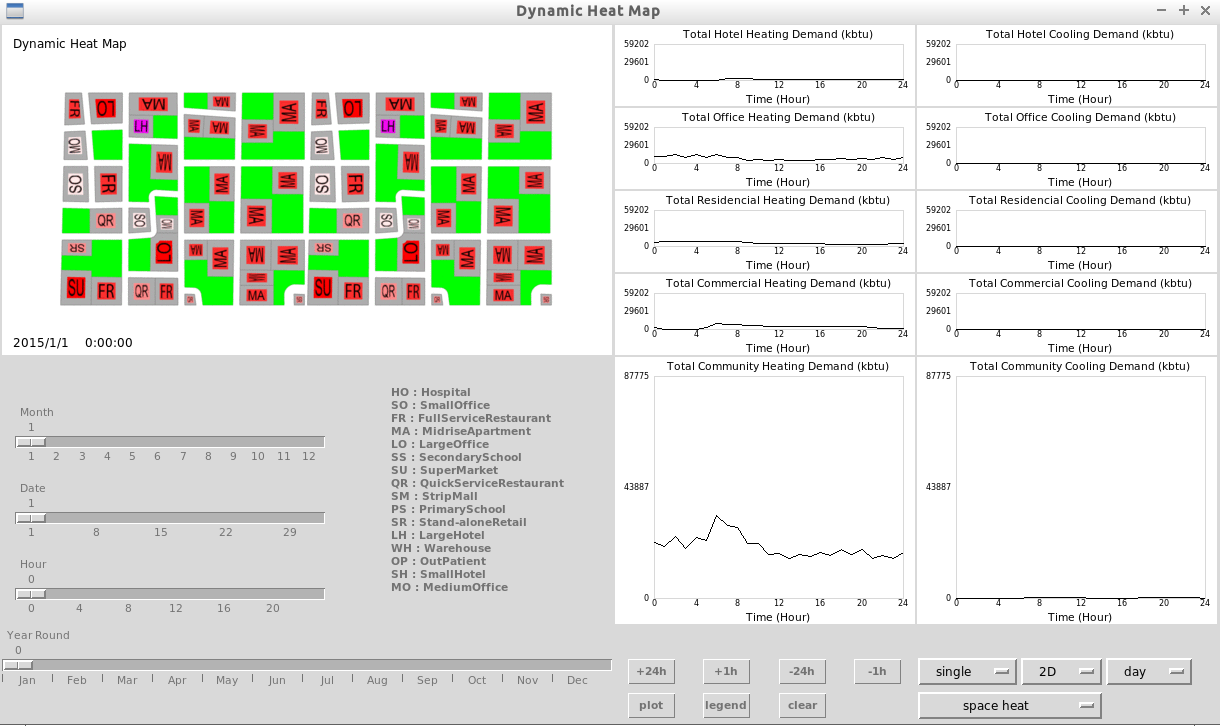
\includegraphics[width=\linewidth]{interface08}
  \caption[Dynamic Energy Map Interface Snapshot]{A snapshot of the dynamic energy map interface}
  \label{fig:interface08}
\end{subfigure}
~
\begin{subfigure}{0.7\textwidth}
  \centering
  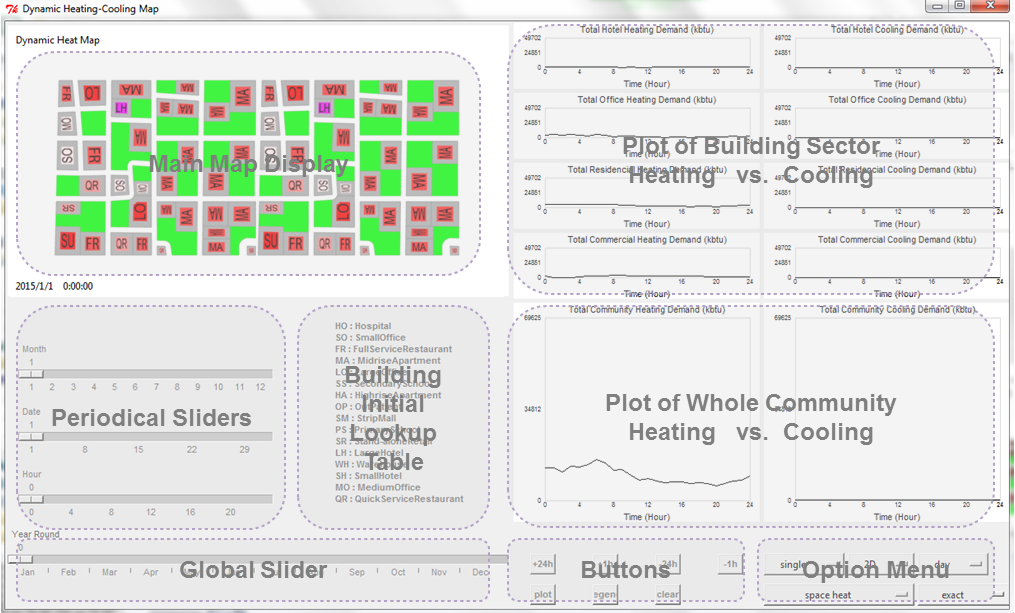
\includegraphics[width=\linewidth]{layout08.png}
  \caption[Dynamic Energy Map Interface Layout]{Dynamic Map Interface Layout}
  \label{fig:layout08}
\end{subfigure}
\caption{Dynamic Map Interface Layout}
\label{fig:interfaceLayout}
\end{figure}

\begin{itemize}
\item A main map display on the upper left that shows the 2D or 3D
  version of the dynamic energy map with energy data encoded as the
  color of buildings. 

\item Four sliders that controls the linear and periodical navigation
  of the map image display and data plot.

\item A ``Building Initial Look-up Table'' in the center bottom that
  defines the two-letter building type initials on the main map
  display window.
\item A series of energy demand plots for four major building sectors
  (top right) and the whole community (lower right).  
\item A series of buttons and option menus on the lower right. 

  The top row of the buttons performs forward (+) or backward (-) time
  navigation with time step of 24h or 1h. The bottom row of the
  buttons contains a ``plot'' button that plots the energy profile
  graphs of the 16 benchmark buildings (if ``single'' is chosen for
  option menu'') or the plot of the aggregated community (if
  ``community'' or ``group'' is chosen), a ``legend'' button that
  shows the current legend, and a ``clear'' button that clears the
  selection in the 2D mode.
\end{itemize}

The following sections will provide more detailed explanation of the
interface.

\subsection {Main Display Window} \label{2d3d} 

As is mentioned in ~\cite{Brownrigg2005}, the choice of 2D
representation vs. 3D representation is one of the debated decisions
in the world of cartographic data
visualization~\cite{Brownrigg2005}. 2D maps are 1) easier to navigate
and 2) the operation of selecting an element or a region is easier to
perform in a 2D map. Another important advantage of 2D map is that it
has better theory support~\cite{Resch2014}: Jacques Bertin defined the
seven visual variables in the graphic sign-system and their
construction rules to effectively convey geographic information
~\cite{Bertin1983}. However the principles and variables of 3D or 4D
maps (space-time map) are not thoroughly
investigated~\cite{Resch2014}. This situation makes the design of 3D
maps more difficult. However 2D maps ``drastically simplify reality
and thus do not give credit to the highly complex capabilities of
human spatial cognition''~\cite{Resch2014}. Regarding this, a 3D map
is rich in geometry representation and can provide realistic
scenes. The realistic scene is important in conveying information to
not only researchers but also the general public. The difference in
surrounding building height and their exterior reflection properties
could influence the exterior shading of a building, so the height and
density distribution of a community could influence its total energy
demand. The correlation of 3D community configurations with difference
in building height, density and exterior surface properties on the
total community level energy performance could also be identified with
a 3D display. The current project does not use the whole-community
energy simulation and this capability of the 3D display is not
demonstrated. Integration with whole-community simulation thus could
be one of the later development of the current project. However, the
3D display can both be an advantage or disadvantage based on the
actual map usage. According to Tufte's data-ink ratio theory, the
extra non-crucial richness of information should be eliminated to make
the most important information stand out~\cite{Tufte83}. For an energy
map, variables such as geothermal energy potential, biomass potential
could be represented as 2D layers while solar energy potential might
be more suitable to be visualized in 3D layers since its performance
is influenced by exterior shading in an urban environment.

For the current dynamic energy map interface, both 2D and 3D
representations are provided for the users to select.  The main map
display window on the top left is used for displaying the 2D / 3D
dynamic map of the conceptual model. The lower left of the main map
display window displays the current time for the image and data
plots. By selecting the 2D / 3D option in the option menu on the lower
right, the user can choose between 2D and 3D display. The 3D display
provides a more realistic view of the community model. The building
geometry is simplified in the current model in order to emphasize the
color changing between frames without introducing distraction from
complicated building geometry. Additional building details or features
could be added to make the display more realistic. In the 2D display,
the user can click on a single building or select a group of buildings
to display their energy profile plots or the aggregated energy profile
plots (\fref{fig:2d3dSelect}).

\begin{figure}[h!]
  \centering
  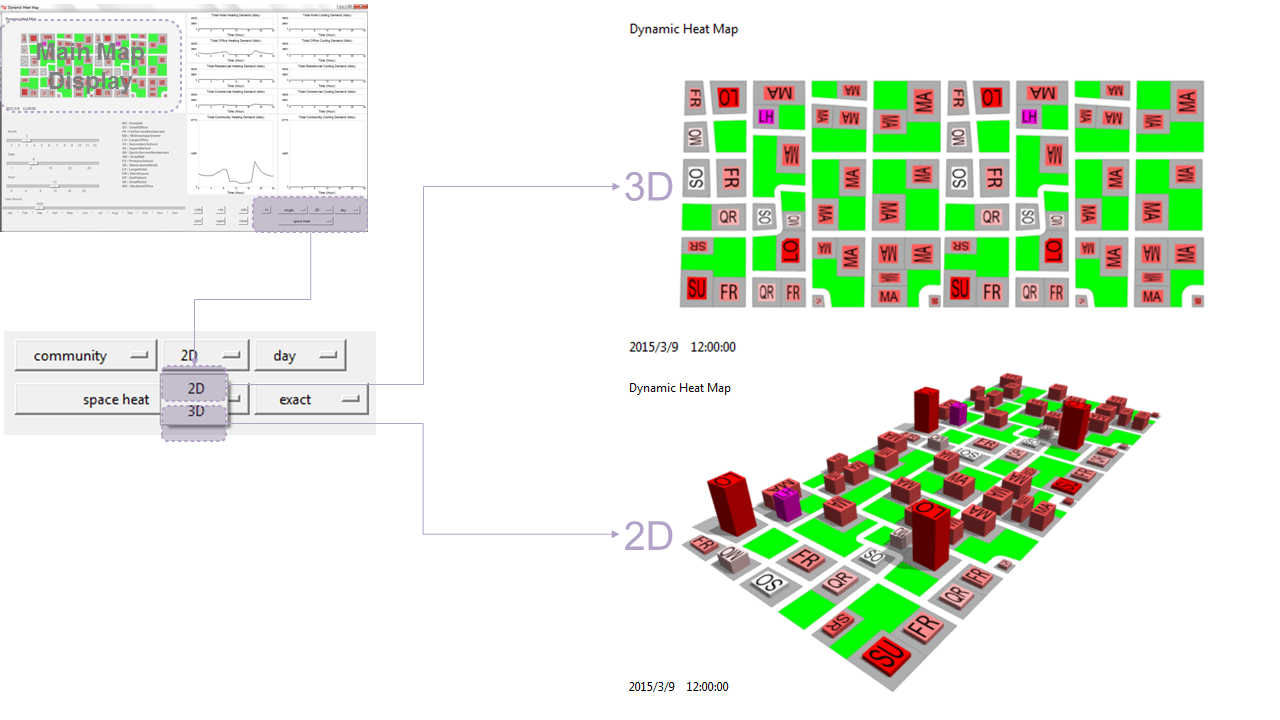
\includegraphics[width=0.7\linewidth]{2d3dSelect.png}
  \caption[Map Display of 2D and 3D]{The current interface provides
    the choices of viewing 2D and 3D map display by toggling the 2D/3D
    option menu}
  \label{fig:2d3dSelect}
\end{figure}

\subsection{Bivariate Map Legend} \label{bivariate}

\subsubsection{Symbol Chosen}
The major reason for choosing the 3D energy dynamic map display is to
use it to provide a more realistic urban environment context.  In the
Dutch Heat map by Dobbelsteen et al.\ , the quantity of energy demand
of each building or region is represented by extruding the building or
region by a corresponding height encoding its energy demand or supply
~\cite{Dobbelsteen2013}. This approach provides an easy way of
aggregating energy demand and supply by adding up geometry height. For
this project this approach was not chosen for the map design because
it creates shape distortion and will impair the goal of providing a
realistic urban environment vision.

In order to represent space heating demand and cooling demand on the
same map, a common map design case is encountered in the current
project: bivariate map design that visualizes the correlation of two
variables on a same map. Elmer points out the challenge of the
bivariate map design as a result of its increased information
density. He presented eight possible types of representation for
bivariate maps (\fref{fig:bivariateExp}): ``shaded cartographer,
rectangle map, bar chart, value by alpha, choropleth with graduated
symbol, bivariate choropleth, spoke glyph and shaded
texture''~\cite{Elmer2012}. In order to incorporate the bivariate map
symbols to the current 3D model without introducing too much shape
distortion, the researcher did not choose the representation with
dimensional changes, i.e. the changing of building height, width,
depth or the size changing of building centroid are not chosen in the
map design of the current project. The choices are the ones that
involves color or texture, i.e. ``bivariate choropleth, value by alpha
and shaded texture'' (\fref{fig:bivariateExp}). Among these three
choices, bivariate choropleth representation has the highest accuracy
rate~\cite{Elmer2012}, hence the researcher chose bivariate choropleth
as the representation of the current map interface design.

\begin{figure}[h!]
  \centering
  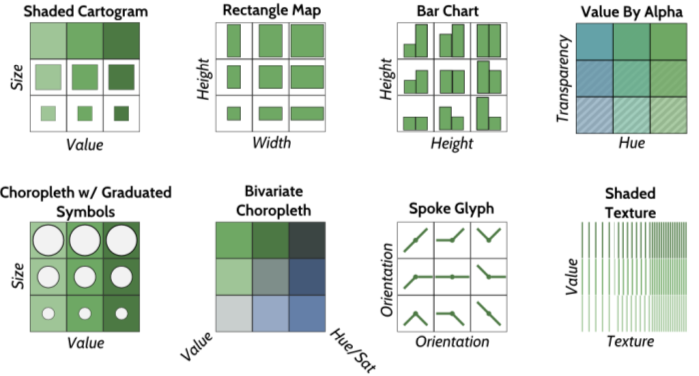
\includegraphics[width=0.7\linewidth]{bivariateExp.png}
  \caption[Bivariate Map Symbol Tested]{The eight bivariate map
    display approaches tested in Elmer's~\cite{Elmer2012} study}
  \label{fig:bivariateExp}
\end{figure}

\begin{figure}[h!]
  \centering
  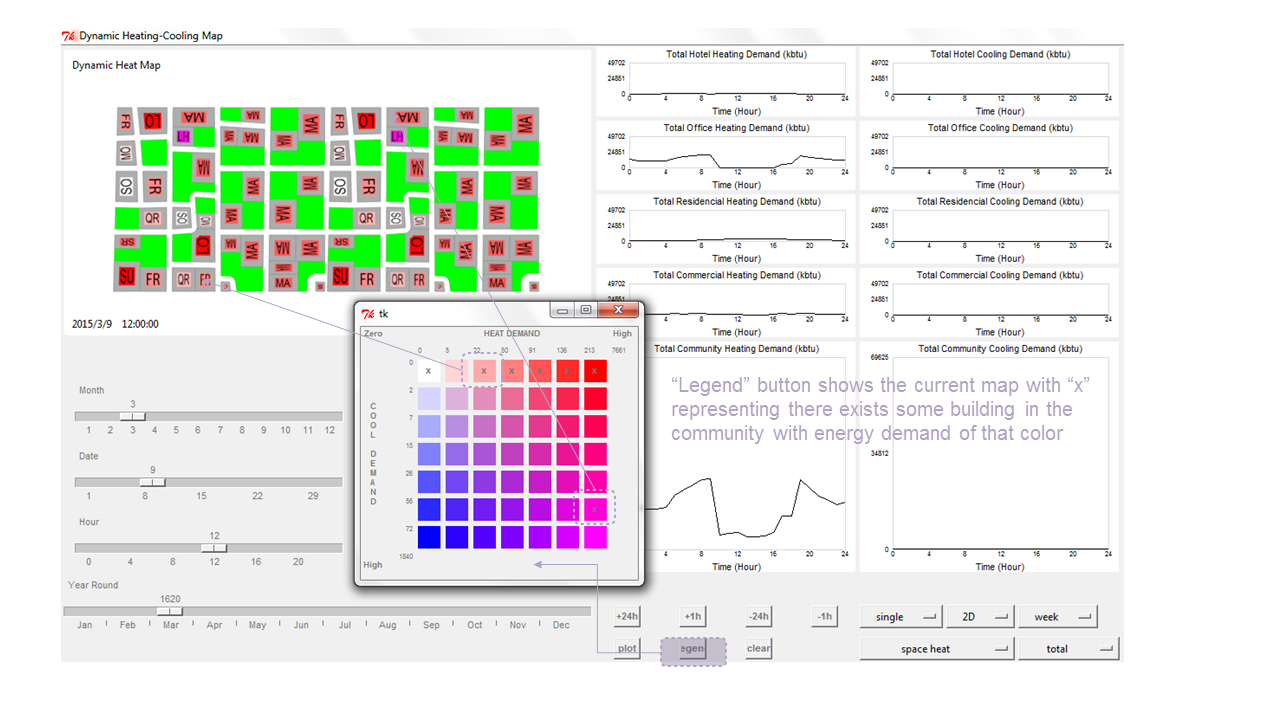
\includegraphics[width=0.7\linewidth]{legend.png}
  \caption[Bivariate Map Legend]{The seven-class-bivariate choropleth
    legend is used in the dynamic energy map interface design with red
    representing high space heating demand, blue representing high
    space cooling demand. ``x'' in the legend corresponds to colors
    appear in the current map display window}
  \label{fig:legend}
\end{figure}

In the current interface design, users can click on the ``Legend''
button and a legend used for encoding the 2D and 3D map will be
displayed. To assist legend reading and color comparison between the
map and the legend, tick marks of ``x'' are added to the legend to
indicate the color appeared in the map \fref{fig:legend}. How to use
the legend to identify the buildings or building groups that have
large energy recovery potential is demonstrated in \sref{useCase1}.

\subsection{Time Sliders and Navigation Buttons}
The lower left section contains a series of sliders for controlling
interactive navigation of the image sequence and the corresponding
data plot.

Harrower and Fabrikant classify time into two types: linear and
cyclic~\cite{Harrower2008}. The former represents the periodical
changes and the latter represents the linear changes of spatial
temporal variables. To address this, the design of the current
interface includes both an overall time navigation utility and time
navigation utilities that facilitate jumps with time steps
corresponding to the natural period of energy data, such as month, day
and hour. This design choice is anticipated to facilitate the
representation of both linear changes and periodical changes of energy
usage in the community.

There are three shorter ``periodical'' sliders on the lower left of
the interface. One unit of position change in the ``month'' slider
results in a forward or backward jump of one month in time. The total
number of positions in the ``month'' slider equals the number of
months in a year (which is the next level of time unit regarding
month).  The jump step for ``date'' slider is one day and the number
of positions in the ``date'' slider is the number of days per
month. Similarly for the ``hour'' slider, the jump step is one hour
and the number of positions in the ``hour'' slider is the number of
hours per day. Suppose the current time in display is 2015/1/1
12:00:00. By moving the month slider, viewers can see the energy
demand in the form of map image and data plot for 2015/2/1 12:00:00,
2015/3/1 12:00:00, $\dots$, 2015/12/1 12:00:00. Similarly, if viewers
pull the ``date'' slider, they can compare the different energy demand
of this hour (12:00:00) throughout the whole month. With the hour
slider, viewers can compare the energy demand between different hours
of a day.

There is a longer ``linear slider'' on the bottom left of the
interface. It has a time step of an hour and a navigation range of a
year (8760 hours). It allows users to globally navigate through all
8760 hours of the year.

There are four buttons (+24h, +1h, -24h, -1h) on the bottom right of
the interface. They provide a micro level adjustment of time.

\subsection{Data Plot}
\subsubsection{Methods to Show Plot}
There are three ways to view energy data plots in the dynamic energy
map interface:
\begin{enumerate}[1)]
\item \textbf{By viewing the right hand side of the interface.}

  The dynamic data plots are directly shown on the right of the
  interface. They depict the energy demand of the four major building
  types (Hotel, Office, Residential and Commercial buildings) and the
  community.

  Space heating and cooling energy demand is displayed in
  \fref{fig:interfaceLayout}. The interface can also display the
  electricity and heating demand for the CHP plant sizing
  application. These plots starts from the current time showing on the
  time sliders with a fixed plotting range of 24h.

\item \textbf{By clicking on the ``plot'' button on the lower right of
    the interface.}

  If the ``single'' option in the option menu is chosen before one
  clicks the ``plot'' button, a data plot will be created for each
  building type (\fref{fig:singlePlot}). If the ``community'' option
  in the option menu is chosen before one clicks the ``plot'', a data
  plot for the community will be created (\fref{fig:communityPlot}).

  \begin{figure}[h!]
    \centering
    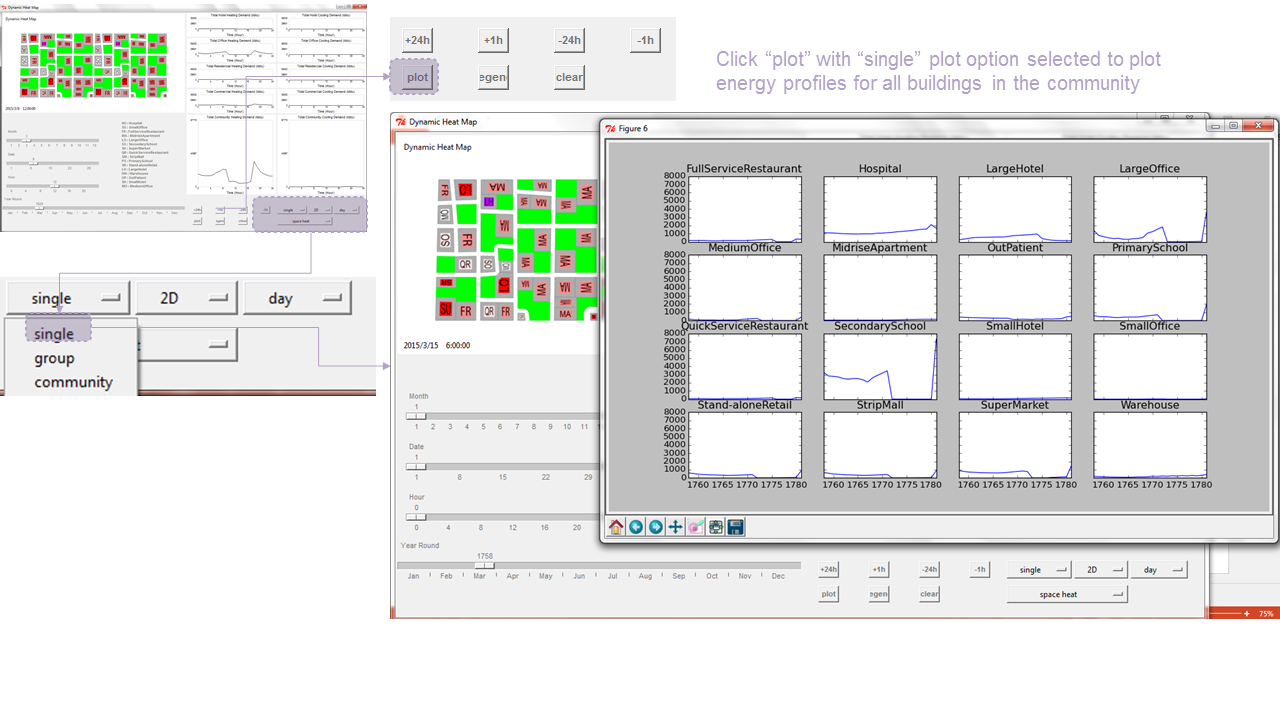
\includegraphics[width=0.9\linewidth]{singlePlot.png}
    \caption[Single Plots of 16 Building Types]{The plot shows the
      space heating energy demand plot of each of the 16 benchmark
      buildings}
    \label{fig:singlePlot}
  \end{figure}

  \begin{figure}[h!]
    \centering
    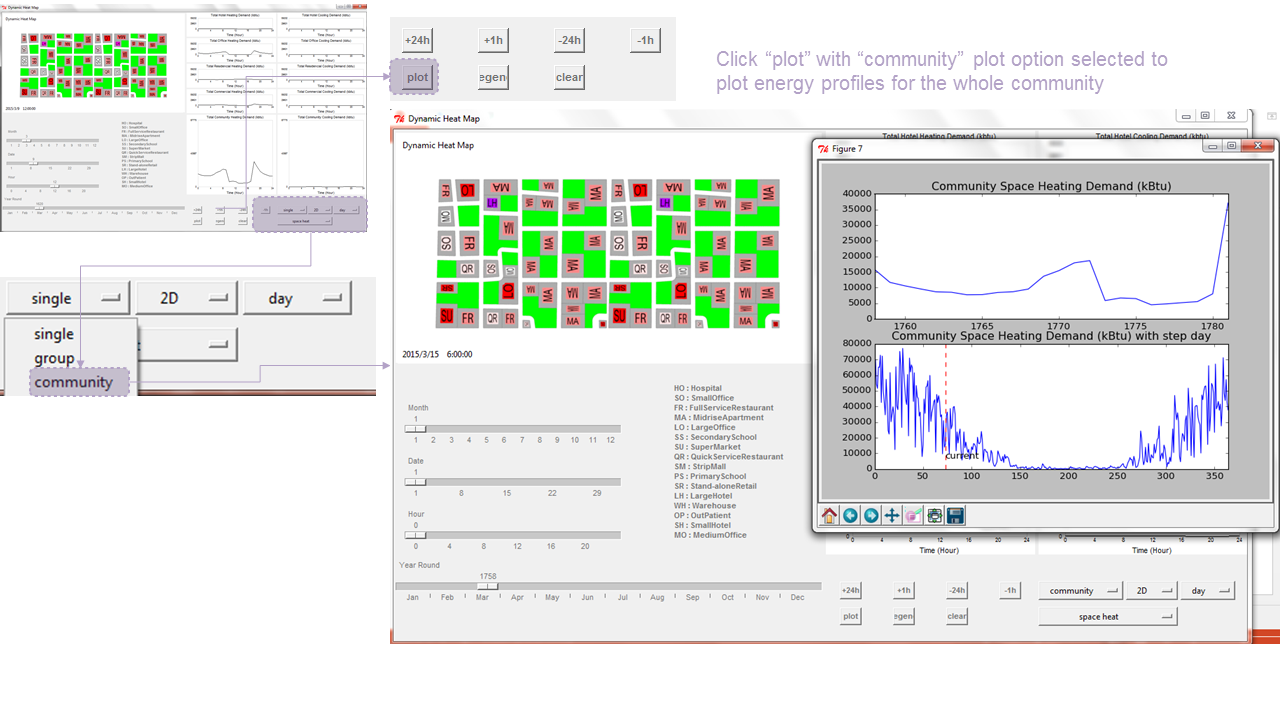
\includegraphics[width=0.9\linewidth]{communityPlot.png}
    \caption[Community Plot]{The plot shows the aggregated space
      heating energy demand for the whole community}
    \label{fig:communityPlot}
  \end{figure}

\item \textbf{By clicking on the building footprint in the 2D map
    display.}

  A building is ``selected'' if the user clicks on its foot
  print. Each new click of a building footprint will add a new copy of
  that building to the selection set. The selection set can be cleared
  by pressing the ``clear'' button. If ``single'' option is chosen in
  the option menu before clicking on a building's footprint, a data
  plot will be created for the building the viewer just clicked on
  (\fref{fig:clickSingle}). If ``group'' is chosen in the option menu,
  each click of a building's footprint will create a data plot for the
  current selection set (\fref{fig:clickGroup}). This function is
  important in assessing the building group level energy recovery
  potential. Users can assess the energy recovery potential of the
  building or building group that rejects heat. They can also assess
  the space heating demand of the group of surrounding buildings of
  the reject heat producers. By comparing these two graphs the users
  can assess the effectiveness of energy recovery strategy in reducing
  the space heating demand of the group of buildings. A demonstration
  of presented in \sref{useCase1}
  
  \begin{figure}[h!]
    \centering
    \includegraphics[width=0.9\linewidth]{clickSingle.png}
    \caption[Show Plot for One Building]{Click on a building foot
      print shows the energy plot of this building}
    \label{fig:clickSingle}
  \end{figure}

  \begin{figure}[h!]
    \centering
    \includegraphics[width=0.9\linewidth]{clickGroup.png}
    \caption[Show Plot for a Group of Buildings]{Click on a building
      footprint shows the energy plot for the selected building group}
    \label{fig:clickGroup}
  \end{figure}

\end{enumerate}

\subsubsection{Providing Temporal Context in Data Plot}

Brownrigg suggested that it is necessary to provide a temporal context
in a space-time map: ``To comprehend how drastically or subtly
something is changing, how fast or slow, in what direction, in
relative to its environment, etc., demands some knowledge of the
history of the change, an awareness of the objects' properties before
and after the change.''~\cite{Brownrigg2005}.

In the current map image display, the temporal context is created by
providing three ``periodical'' slider bars that allows the user to
jump with time steps of month, day and hour. 

In data plots, the temporal context is created by providing a
``longitude'' and ``latitude'' comparison of energy demand.
``Longitude'' here refers to the comparison of adjacent time spots. It
shows what the states of the direct future or past comparing to the
state of the current time. ``Latitude'' here refers to the comparison
of the current time spot with all similar time instances, for example,
all 12:00:00 energy demand of the year. It shows how the current
instance differ from similar instances.

For the current interface design, the top plot presents a longitude
temporal context of the energy demand of the incoming 24h, week or
month. Corresponding to the duration of time of the top plot (24h or
one week or one month), the bottom plot presents the latitude demand
context of the same hour with a step of one day, one week or one
month. For example, in \fref{fig:dayContext}, the top plot shows the
Space Heating Demand for Large Office from 2015/3/9 12:00:00 to
2015/3/10 11:00:00, with a duration of 24h. The bottom plot shows the
energy demand of the Large Office for all 12:00:00 of the 365 days of
the year (the red dot line indicates the 12:00:00 of around the 70th
day of the year, which is the date of Mar. 9th).

\begin{figure}[h!]
  \centering
  \includegraphics[width=0.9\linewidth]{dayContext.png}
  \caption[Data Plot with Duration / Step of One Day]{The data plot
    presents the longitude and latitude comparison of energy demand,
    the top plot presents a temporal context of the energy demand of
    the next 24h, the bottom plot presents the time context of the
    demand of the same hour throughout the 365 days of the year}
  \label{fig:dayContext}
\end{figure}

\begin{figure}[h!]
  \centering
  \includegraphics[width=0.9\linewidth]{changeT.png}
  \caption[Data Plot with Different Duration / Step]{By changing
    option in the option menu. User can choose to display a longitude
    latitude comparison with the time unit of day, week or month. The
    top plot shows the energy demand for the next day, week and month
    from left to right; the bottom plot shows the energy demand of
    this hour in the 365 days of year, 52 weeks of a year or the 12
    months of a year from left to right}
  \label{fig:dayContext}
\end{figure}

By providing the temporal context, the viewers are provided with a
general understanding of whether the changing of energy demand
behavior is drastic or subtle and whether a drastic change is coming
and whether the current demand is high, low or moderate comparing to
the overall distribution over time and space.

\pagebreak
\section{Use Case Demonstrations}
\subsection{Use Case I: Identification of Energy Recovery Opportunity}\label{useCase1}
In this section, the researcher present a general approach on how to
use the dynamic energy map interface to identify the energy recovery
opportunities. The process of space cooling will produce reject
heat. As is explained in \sref{sec:inputRecover}, the ammount of
cooling-induced reject heat is positively corelated to the cooling
demand. Thus a building with high cooling demand will also have a
large amount of reject heat. The reject heat from this building or
group of buildings could possibly be recovered for use within the
building such as pre-heating water or outside air or be transmitted to
other buildings that have space heating demand so that the total space
heating demand of the group of buildings could be reduced.

For the interface design in the current study, the researcher used a
bivariate color ramp in space heating and cooling energy demand data
representation that depicts the hourly space heating and space cooling
demand on the same map (\fref{fig:legend2d}) . Red represents high
heating demand and blue represents high cooling demand. The closer the
color cell is to the top, the lower cooling demand. The closer the
color cell is to the left, the lower heating demand. The cells on the
diagonal line (purple colored cells) represent buildings that have
relatively similar heating and cooling demand. The cells to the upper
right of the diagonal represents buildings that are heating dominated
and the cells to the lower left of the diagonal represent buildings
that are cooling dominated. The current breakpoints are decided
through the ``Quantile method'' ~\cite{GIS_Jenks2014} for
demonstration.

\begin{figure}[h!]
  \centering
  \includegraphics[width=0.7\linewidth]{legend2d.png}
  \caption[Heating-Cooling Map Legend Illustration]{The bivariate
    color ramp displays two variables at the same time: space heating
    and space cooling. It better displays the co-relation between
    these two variables and thus helps users to identify energy
    recovery opportunities}
  \label{fig:legend2d}
\end{figure}

With the dynamic energy map, the buildings colored in one of the
colors in the bottom rows of the legend are buildings with high
cooling demand. With the dynamic energy map, users can identify the
potential reject heat suppliers and consumers over time
(\fref{fig:highCooling}).

\begin{figure}[h!]
  \centering
  \includegraphics[width=0.7\linewidth]{highCooling.png}
  \caption[Identify Buildings with High Cooling Demand]{In the
    demonstration, buildings with a high cooling demand have colors on
    the bottom rows of the legend, thus Large Hotel and Large Office
    are identified as potential reject heat energy suppliers}
  \label{fig:highCooling}
\end{figure}

Users can then calculate the ``energy recovery potential'' in the
dynamic energy map with a specified time duration and step.  In the
example of \fref{fig:ERP}, users identify the Large Office and the
Large Hotel as reject heat suppliers and calculated their aggregated
energy recovery potential for the 16th week of the year in the graph
on the left. Then they calculated the space heating energy demand of
the group of surrounding buildings of reject heat suppliers: two First
Service Restaurants, two Midrise Apartment and one Small Hotel. 

By comparing the two graphs, users can see that the peak of the energy
recovery potential is about four times of the peak of the space
heating demand of the group of surrounding buildings. They can also
observe that there are two peaks for space heating demand of the
surrounding building group but only one peak for the energy recovery
potential. There are some difference in the weekly pattern of the
reject heat supply and the space heating demand: the last two days of
the week has very little reject heat but the space heating demand is
relatively high. We can also see that the peak of reject heat does not
occur at the same time with the space heating demand peak: in the
2800th hour, reject heat (in the graph on the left) reaches its peak
while space heating demand on the right is zero. With the dynamic
energy map, users can identify complicated non-coincidence in the
supply and demand of reject heat. This information could help users
conduct more detailed heat recovery strategies and assess the thermal
energy storage devices.

\begin{figure}[h!]
  \centering
  \includegraphics[width=0.7\linewidth]{ERP.png}
  \caption[Calculate Energy Recovery Potential]{The users can
    calculate the energy recovery potential of the group of reject
    heat suppliers (Large Office and Large Hotel). They can also
    calculate the total heat demand of the surrounding buildings with
    space heating demand (two FirstService Resturant, two Midrise
    Apartment and one Small Office).}
  \label{fig:ERP}
\end{figure}

\subsection{Use Case II: Sizing CHP Plant}
With the Dynamic Energy Map that depict the spatial temporal load
variation, one will idealy be able to 1) idendify anchor load
buildings, 2) conduct better design of local load balancing, 3) size
the co-generation CHP plant

\begin{itemize}
\item Identify anchor load buildings
  
  To achieve this function, the map should be able to make the
  building with persistant high heating or cooling demand stand
  out. Thus the color scheme assigns vibrant colors to high demand and
  white to low demand. The break points of ``high'' demand remains to
  be decided in further project development. For the current
  implementation, the break point is acquired with the quantile
  classification method.

  Although with the box plot of heating demand (\fref{fig:SH}), the
  buildings with high consistently high heating demand through its
  high median and 25 percentile, a more intuitive interpretation is
  still needed to convey information to people with less statistical
  background. From the animated version of the dynamic energy map
  (link to 2d map, link to 3d map) the Large Office, the Large Hotel
  and the Midrise Apartment forms a high heat demand region, these
  could be potential locations for making a connection to a district
  system.

  \begin{figure}[h!]
    \centering
    \includegraphics[width=0.7\linewidth]{heatPowerDemand.png}
    \caption[Comparing Community Heating and Electricity Demand]{In
      this example, the users compare the week-wise heating and
      electricity demand}
    \label{fig:heatPowerDemand}
  \end{figure}
\item Size a CHP plant 

  Two variables are crucial in sizing a CHP plant: 1) the heating
  demand including space heating and service hot water 2) electricity
  demand. For the current dynamic energy map interface, a 2D/3D
  choropleth map are presented in the main map display window with the
  heating demand and electricity demand encoded with a seven-class
  bivariate choropleth legend as in \fref{fig:CHPHeating}. The dynamic
  plot on the right of the interface depicts the heating and
  electricity demand of the four building sectors and the community .

  The user can also inspect heating energy and power demand of he
  community with different time span and different aggregation
  method. For example, they can compare the heating and power demand
  for a week and see if the demand align. In \fref{fig:CHPHeating},
  users can see the peak heating demand for the ninth week is about
  the same level as the peak demand for the electricity. However,
  their weekly behavior is different: the heating demand for the
  second half of the week are relatively low but the electricity
  demand is relatively high. The lower graph also shows that the
  annual peak demand of electricity occurs during the time when the
  community has the lowest heating demand. This poses the challenge
  for the district energy system with Co-generation local plant and
  the necessity for thermal energy storage devices in a district
  energy system.

  \begin{figure}[h!]
    \centering
    \includegraphics[width=0.3\linewidth]{legendCHP.png}
    \caption[Legend for Heat and Power Map]{Legend for Heat and Power
      Map}
    \label{fig:legendCHP}
  \end{figure}

  \begin{figure}[h!]
    \centering
    \includegraphics[width=0.7\linewidth]{CHPHeating.png}
    \caption[Interface for CHP Sizing]{In this example, the users
      compare the week-wise heating and electricity demand}
    \label{fig:CHPHeating}
  \end{figure}

\item Local load balancing

  Apart from the information for the minimum and maximum value of the
  heating and electricity demand of the community, more specific
  heating and electricity demand of single buildings and building
  groups are also available. This could be used to design micro-scale
  CHP equipment or to locate thermal energy storage devices and to
  size their storage capacity.  For the micro-scale CHP equipment
  design, a load balancing in the level of a building group could make
  the micro-scale CHP equipment operate in its high efficiency output
  for a longer period.
  
  To achieve this, the program enable users to select a subset of the
  existing buildings and creates the aggregated heating load plot for
  the selected building group (within the specified time period). 

  The user will first identify some cluster of buildings, in which
  there is a pattern of building that turn red sequentially but not
  simultaneously. Then they can check the building demand profile by
  clicking on the building footprint in the 2D map
  (\fref{fig:seeLoad}).

  \begin{figure}[h!]
    \centering
    \includegraphics[width=0.7\linewidth]{seeLoad.png}
    \caption[Check Heating Load]{Users can check the building energy
      demand (thermal or electricity) by clicking on the building foot
      print in the 2D map and the interface will show the plot of the
      energy demand profile within a period (the example is showing
      the demand for a 24h hour period)}
    \label{fig:seeLoad}
  \end{figure}

  Alternatively, they can first open the window that displays the 24h
  period energy demand graph (hourly gas heating energy in the
  following example) for all of the 16 prototype buildings and see if
  there are some building types that have demand complimentary (so
  they have a rough idea of what is a ``good building combination''
  (\fref{fig:plotAll}) at this time that could be a candidate for load
  balancing) and they will look at the map and search for this ``good
  combination''.

  \begin{figure}[h!]
    \centering
    \includegraphics[width=0.7\linewidth]{plotAll.png}
    \caption[Check All Heating Load Plot]{Users can plot all building
      energy demand profile (heating gas demand for the example) and
      search for ``good cobimations'' that have compensate load
      profile}
    \label{fig:plotAll}
  \end{figure}

  After the qualitative experimentation, users can select a group of
  building by clicking on the building footprint and the program will
  output a graph of aggregated load

  \begin{figure}[h!]
    \centering
    \includegraphics[width=0.7\linewidth]{seeAggDemand.png}
    \caption[Plot Aggregated Demand]{In this example, users selected
      the Stand-alone Retail and the Large Office and plots of each
      single building and the aggregated demand of the two buildings
      are displayed}
    \label{fig:plotAll}
  \end{figure}

\end{itemize}

\begin{comment}
\section{Future Trends}
Harrower and Fabrikant mentioned that the chanllenge of using animated
maps is the overflow of information and the vulnerability to
distraction~\cite{Harrower2008}. One example mentioned by Harrower and
Fabrikant is the comparison of color on the map and that on the legend
becomes difficult for animated maps as a result of the changing of
images. They proposed the audio legend approach of strengthening
information convey with minimized
distraction~\cite{Harrower2008}. This might become one of the next
extensions of the current Dynamic Energy Map interface design.

They also suggested that the difference in time should have different
visual representations in data display~\cite{Harrower2008}. Peuquet
claimed that ``The development of temporal analytical capabilities in
GIS such as temporal queries requires basic topological structures in
both time and space''~\cite{Peuquet1994}. Thus the different spatial
representation seems to be a natural choice for adapting to different
temporal resolution and scale.



The non-interactive animation could be found
\href{http://www.armechxyj.com/energy-mapping.html#redblueAnime3d}{through
  this link}.
\end{comment} 

% Chapter 7

\chapter{Findings and Discussion} % Main chapter title

\label{Chapter7} % For referencing the chapter elsewhere, use \ref{Chapter1} 

\lhead{Chapter 7. \emph{Findings and Discussion}} % This is for the header on each page - perhaps a shortened title

%----------------------------------------------------------------------------------------
\section{Insight of energy mapping with time information}
The document presents an approach of implementing a dynamic energy map
with a focus on visualization of high spatial-temporal energy demand
data of single buildings, building groups and the whole
community. 

In order to visualize the energy demand data to better convey the
dynamic energy demand changing, a detailed analysis of the input
demand data profile of each building type and the aggregated community
was conducted in \sref{boxPlot}. From this analysis, we observed a
great variation in the demand profile distribution between different
building types and a strong skew of the energy demand profile of the
whole community. Log scaling and data classification with the quantile
method was adopted to cope with this skewed data distribution in the
design of the conversion from energy demand to their color encoding.

An interface is designed to visualize the 2D/3D map images that
encodes energy demand information with a bivariate choropleth
legend. A series of data plot functions accompany the map image
display to provide quantitative information. The data plot provides
different level of temporal and spatial aggregation method that serve
more generic purpose of data analysis and visualization so that it
suits the need of the target user group: researchers in energy related
fields who have different research interests and focuses.

% bookmark
Through the dynamic energy map, many detailed spatial temporal energy
demand pattern can be revealed:
\begin{itemize}
\item The daily peak energy demand arrival time is different for
  different building types
\item The aggregation of peak demand is not a simple addition of peak
  demand of the peak of each component building's peak demand
\item The reject heat supply peak is different from the space heat
  demand peak
\item The heating and electricity demand for the community have very
  different weekly demand behavior
\end{itemize}
\section{Limitations and Further Development}
The current project presented a initial implementation of a dynamic
energy map with the focus on spatial-temporal energy profile
visualization. Due to limited time and resources, there are many to be
realized in the next stage development:

\begin{itemize}
\item Input data

  Community level energy simulation is not used in the energy profile
  generation. This leads to simplified assumptions of micro-climate in
  an urban environment. The building height and urban density could
  influence the exterior shading and could influence buildings'
  heating and cooling demand. The urban environment configurations of
  urban density and the spatial distribution of building height could
  potentially be conveyed with the dynamic energy map with 3D map
  sequences. However as a result of the stand-alone assumption, this
  layer of information is not demonstrated in the dynamic energy map
  in the current project.

  The current project focuses mainly on the demand side information,
  except that the cooling-induced reject heat is calculated. One of
  the major goal of energy mapping is to make the energy supply meet
  the energy demand. In order to fully realize the function of an
  energy map, adding supply side information is crutial. In the
  further development of the project, supply side information
  especially renewable energy supply assessment should be added to the
  dynamic energy map. This could pose new challenges of map design and
  data visualization as a result of the added layers of
  information. Further investment of proper spatial-temporal data
  visualization method could also become another topic of the next
  stage development of the project.

  The matching of energy demand and supply include not only matching
  in energy quantity but also energy quality in terms of exergy
  ~\cite{Dobbelsteen2013}. The current map interface does not contain
  exergy information. Further development could add exergy information
  in order to facilitate the design of energy cascading.

  When 

\item Visualization

  In the data classification step, the break point is acquired with
  quantile classification method as is discussed in
  \sref{dataClassification}. Further analysis of building science
  context based break point selection, such as critical value for
  mechanical equipment sizing or minimum recoverable heat considering
  transmission loss etc., should be taken into consideration in the
  next stage development of the project.
  
\item Data Sharing
  
  As is envisioned in the study of Baird et al.\ , an on-line platform
  is needed to facilitate data access, model sharing and advanced
  analysis~\cite{baird2014}. The current implementation of the dynamic
  energy map is a stand-alone tool. Bringing the current dynamic map
  to be an online map could be the next stage development.

\item Technical issue

  As a result of the dependence on an existing modeling software for
  image generation, user could not create community design and compare
  design alternatives on the current interface; user control over data
  classification and legend selection are not realized either. To
  solve this problem, a 3D model importing and rendering function
  should be added to the current map to facilitate the
  performance-based community energy planning.

\end{itemize}
%% Chapter 5

\chapter{Literature Study on Map Design and Data
  Visualization} % Main chapter title

\label{Chapter5} % For referencing the chapter elsewhere, use \ref{Chapter1} 

\lhead{Chapter 5. \emph{Map Design}} % This is for the header on each page - perhaps a shortened title

%----------------------------------------------------------------------------------------
\subsection{Animated Maps}\label{anime}
Animated maps are proven to be more powerful in conveying the
spatial-temporal pattern than static maps~\cite{McEachern1998}.

In order to represent dynamic geographic processes, map animation is a
natural choice. It was introduced to the world of cartography in
1930s~\cite{Harrower2008}. The major application of animated maps
include: 1) demonstrating the dynamic process of geographic events
(weather maps in weather forecasting is such an example) 2) assisting
pattern recognition and knowledge development for scientific
researches. The study by Dorling and Openshaw is an example of 
application 2), where they discovered new leukaemia hotspots through
animated maps~\cite{Dorling1992}.

Animated maps are not superior to static maps, it is just they are
good at different aspects of information convey. The animated map is
advantageous in demonstrating the changes between frames rather than
the absolute value represented in each frame~\cite{Dorling1992}. It is
proved to be more powerful in convey the spatial-temporal pattern than
static map~\cite{McEachern1998}.

Harrower and Fabrikant mentioned that the chanllenge of using animated
maps is the overflow of information and the vulnerability to
distraction~\cite{Harrower2008}. One example mentioned by Harrower and
Fabrikant is the comparison of color on the map and that on the legend
becomes difficult for animated maps as a result of the changing of
images. They proposed the audio legend approach of strengthening
information convey with minimized
distraction~\cite{Harrower2008}. This might become one of the next
extensions of the current Dynamic Energy Map interface design.

They also suggested that the difference in time should have different
visual representations in data display~\cite{Harrower2008}. Peuquet
claimed that ``The development of temporal analytical capabilities in
GIS such as temporal queries requires basic topological structures in
both time and space''~\cite{Peuquet1994}. Thus the different spatial
representation seems to be a natural choice for adapting to different
temporal resolution and scale.

They classify time into two types: linear and cyclic. Upon this
consideration, the design of the current interface include both an
overall time navigation utility and time navigation utilities that
facilitate jumps with time steps corresponding to the natural period
of energy data, such as month, day and hour. This design choice
is anticipated to facilitate the representation of both linear changes
and periodical changes of energy usage in the community.

The level of user control of playback behavior of animated maps is
also debatable. Some claim providing the full freedom of adjusting
this feature can enhance pattern understanding~\cite{Nelson1998}. But
others argue that this control will reduce time animation to still
images and impair its ability in conveying temporal changes
~\cite{Lowe2004}. In the current dynamic map project, both the
interactive version and the non-interactive version is provided: the
non-interactive version (a map animation) is accessible through
\href{http://www.armechxyj.com/energy-mapping.html#redblueAnime3d}{here}. The
interactive version is provided as a stand-alone Python program.

\subsection{Spatial Temporal Data Analysis}\label{stDataAnalysis}
In order to better utilize the power of Dynamic Maps, one has to
understand the special features of spactial-temporal data and the
methods of how to use spactial-temporal data. This leads to the
literature study of the following section of spatial temporal data
analysis.

One temptation of analyzing spatial-temporal data is to aggregate them
into ``time periods'' and ``zonal entities'' and then use the static
analysis method to analyze the aggregated data~\cite{Dorling1992}. The
problem of this approach is 1) it increases the sensitivity
(i.e. minor changes in input causes dramatic changes in output) and 2)
it removes the ``dynamic'' feature of a dynamic.
map~\cite{Dorling1992}.

One layer of the goal of a space-time map is to make ``complex dynamic
process'' visible, in the hope of letting observers comprehend the
dynamics of data presented and to gain a general insight. Baring this
goal in mind, Dorling and Openshaw suggested a noise removal or data
smoothing in both the time and space dimension before the actual map
creation~\cite{Dorling1992}.

\section{Data Classification}\label{dataClassification}
In order to write the data classification routine for the
demonstration of dynamic energy map in the current study, the authors
conducted a brief survey of the commonly used GIS software for
commonly applied data classification method. The software surveyed in
the study include: ArcGIS~\cite{GIS_Jenks2014}, GRASS
GIS~\cite{GRASSGIS2008}, gvGIS~\cite{gvGIS2011}, and QGIS. The data
classification method adopted by the surveyed software in creating a
thematic map include: 1) equal interval, 2) quantile 3) Jenks 4)
Standard Deviation 5) pretty breaks 6) manual interval (use context
specific break point values). The common data classification method
shared by all surveyed instances are ``Equal Interval'', ``Quantile''
and ``User Defined''. Therefore we chose to implement the ``Equal
Interval'' and ``Quantile'' method in the current project.

\begin{table}[h!]
  \centering
  \begin{tabular}{r|c c c c c c}
    \hline
           & Equal Interval & Quantile & Jenks & Pretty Breaks & StDev & User Defined\\
    \hline
    ArcGIS &      o        &    o     &  o    & x &  o  &   o  \\
 GRASS GIS &      o        &    o     &  x    & x &  o  &   o  \\
     GVSIG &      o        &    o     &  o    & x &  x  &   o  \\
      QGIS &      o        &    o     &  o    & o &  o  &   o  \\
    \hline
  \end{tabular}
  \caption{Data Classification Method (o: yes, x: no)}
  \label{tab:classify}
\end{table}

\begin{comment}

``Data Visualization with Spacetime Maps'', Richard L. Brownrigg, 2005
(read further later on)

\grey{To be continued later:
\begin{enumerate}[label*=\arabic*.]
\item ``Geographic Visualization: Designing Manipulable Maps for
    Exploring Temporally Varying Georeferenced Statistics'', MacEachren et al.\
\item ``Strategies for the Visualization of Geographic Time-Series
    Data'', Mark Monmonier, 2011
\item ``Evaluation of Methods for Classifying Epidemiological Data
    on Choropleth Maps in Series'', Brewer and Pickle, 2002
\end{enumerate}}
\end{comment}



However, the level of user control of playback behavior is debatable
according to previous literature about animated maps. Some claim
providing the full freedom of adjusting this feature can enhance
pattern understanding~\cite{Nelson1998}. But others argue that this
control will reduce time animation to still images and impair its
ability in conveying temporal changes ~\cite{Lowe2004}.
%% Chapter3

\chapter{Building from Previous Work} % Main chapter title

\label{Chapter3} % For referencing the chapter elsewhere, use \ref{Chapter1} 

\lhead{Chapter 3. \emph{Preliminary Design}} % This is for the header on each page - perhaps a shortened title

%----------------------------------------------------------------------------------------
Looking back at the static energy mapping instances, the energy demand
and supply depicted on the map are mainly average, peak or total
values. With these information alone, the time-dependent feature of
energy demand and supply is missing from the coversation.

(add more)

As is mentioned in the introduction, a dynamic energy map has four
major functions: 1) holding, 2) visualizing and 3) analyzing community
level high spatial-temporal resolution energy demand and supply data
4) connection to simulation engine for iterative performance
analysis. 

In the initial instance of Dynamic Energy Map by Baird et al.\
~\cite{baird2014}, function 1) of holding spatial-temporal (although
with low temporal resolution) energy data is realized by processing
the energy simulation data with Microsoft excel and importing the csv
file including ``building name, total conditioned area annual, energy
use intensity, annual and monthly peak demand''. The further
improvement of the current project is to make the geo-database hold
more high resolution energy data, meaning the 8760 hourly energy data
should be contained in the dynamic energy map.

Function 4) of connecting to building simulation data is also realized
by importing simulation result csv files to the geo-database (although
with low temporal resolution).

For function 3), the feasibility analysis of a district energy system
is performed in a stand-alone excel tool~\cite{baird2014} but it is
possible that the analysis result could be linked in to the
geo-database as the energy simulation result. 

For function 2), the spatial and temporal information are visualized
separately in the Lower District Hill Project: the spatial information
of 3D building geometry and location could be visually inspected in
the geo-database but not the hourly energy consumption information. 2)
The temporal visualization of energy demand is done separately in the
excel screening tool as 3D graphs, but no spatial context is present
and the spatial dimension is then lost. The authors thus identified
the crucially missing function: the visualization of such a
spatial-temporal changing of energy behavior as the major goal of the
current project.

\begin{figure}[h!]
  \centering
  \includegraphics[width=0.7\linewidth]{interface08.png}
  \caption[Dynamic Energy Map Display]{Unified Dynamic Energy Map
    Display System}
  \label{fig:interface08}
\end{figure}

%----------------------------------------------------------------------------------------
%	THESIS CONTENT - APPENDICES
%----------------------------------------------------------------------------------------

\addtocontents{toc}{\vspace{2em}} % Add a gap in the Contents, for aesthetics

\appendix % Cue to tell LaTeX that the following 'chapters' are Appendices

% Include the appendices of the thesis as separate files from the Appendices folder
% Uncomment the lines as you write the Appendices

%uncomment in final file
% Appendix A
\chapter{Implementing Dynamic Energy Map in
  CityEngine} % Main appendix title

\label{AppendixA} % For referencing this appendix elsewhere, use
                  % \ref{AppendixA}

\lhead{Appendix A. \emph{Implementing Dynamic Energy Map in CityEngine}} % This is for the header on each page - perhaps a shortened title
\section{General Introduction}
The following document records the method of using CityEngine to
visualize the dynamic energy (heating energy in kwh for this document)
changes with a slider bar embeded in the CityEngine software. To be
more specific, users will be able to navigate through the 8760 hour of
a year with a time slider and see the color-coded energy consumption
data for all buildings in the community model for the hour the slider
cursor rest at. The detailed rule file is included in \aref{AppendixB}.

The general process is to find a base map if it is a real site or
generate a random urban environment layout if it is a conceptual
setting. Add attributes of ``landuse'' and ``time'' to the building
lot. Then write a rule file with energy consumption data (or the color
representation of each energy consumption data) for each building type
held in string lists in the rule file and then apply the rule files to
the building lot. Finally set the attribute of ``landuse'' and
``time'' in the rule file to be driven by the value of the object
attribute ``landuse'' and ``time''. The ``time'' attribute is to index
into the string list of energy profile (in rule files) for each
building type. For example, when the ``time'' attribute of all building
blocks are set to 10, all the buildings in the community model will
change its color to the color representing its heating energy
consumption in the 10th hour (zero-indexing) of the year.

Each step will be explained in more details in the following session.
\section{Explaining Each Steps}
\subsection{Create a Urban Environment Layout}
If one is working with a real project, an OSM Map~\cite{OSM2015} will
be a good choice for a base map. The OSM file contains many useful
attribute such as street center line, building name, elevation etc. It
is of xml format and is easy to manipulate as text files, which makes
it easier to work with and less bulky comparing to ArcGIS gdb
files. \fref{fig:osmCampus} is an example of the CMU Campus OSM Map.

\begin{figure}[h!]
  \centering
  \includegraphics[width=0.7\linewidth]{osmCampus.png}
  \caption[CMU OSM Map]{CMU OSM Map~\cite{OSM2015}}
  \label{fig:osmCampus}
\end{figure}

If it is a conceptual setting, then create a random city of proper
size using ``grow street'' function with some clean-ups
(\fref{fig:randCity}).

\begin{figure}[h!]
  \centering
  \includegraphics[width=0.7\linewidth]{randCity.png}
  \caption[Conceptual City Lots]{Conceptual City Generated with
    CityEngine}
  \label{fig:randCity}
\end{figure}
\subsection{Add Attributes to Building Lots}
To implement the function of a time slider-bar that navigates and
shows energy consumption for each building in each hour of the year,
two additional attributes are needed: 1) ``time'' attribute of type
float (ideally we would like it to be integer but there is no integer
types in object attribute) ranges from 0 to 8760 (not inclusive) that
represents the hour of a year and 2) ``landuse'' attribute of type
float (since no integer type is available) that represents the land
use type of the lot.

Adding these two attribute could be done either inside an OSM base map
or inside CityEngine.

The typical way to add a building attribute can be done by selecting
all building lots and right click one of the Object attributes and
select "Add Object Attribute" to add new attributes.

If an OSM base map is available with building footprint information,
adding attributes can be achieved within OSM maps by one searching for
\texttt{"<tag k="building" v="yes"/>"} and add two new tags after this
line:\\
\texttt{"<tag k="time" v="0"\/>"}\\
\texttt{"<tag k="landuse" v="0"\/>"}\\

\subsection{Importing Base Map (Optional)}
If one is working on a real project, one can add an geo-referenced
terrain image to make the model more realistic. In the following
example, the terrain geo-tiff was retieved from PASDA
website~\cite{PASDAImagery2013} according to the ``Allegheny County
Imagery 2013 - Tile Index''. The image showing the area of interest is
clipped in ArcMap and imported as a geo-referenced image (.tif) to
CityEngine (\fref{fig:geotif}).

\begin{figure}[h!]
  \centering
  \includegraphics[width=0.7\linewidth]{geotif.png}
  \caption[Geo-tif in CityEngine]{Example of Geo-referenced Image in
    CityEngine}
  \label{fig:geotif}
\end{figure}

After importing geo-referenced image, OSM map could be imported and a
working base was formed (\fref{fig:geotifOSM}).
\begin{figure}[h!]
  \centering
  \includegraphics[width=0.7\linewidth]{geotifOSM.png}
  \caption[Geo-tif with OSM Map]{Geo-tif with OSM Map}
  \label{fig:geotifOSM}
\end{figure}

\subsection{Writing Rule File for Building Generation}
We used ``time'' as the index into the string array that holds the
hourly heating energy consumption data. By setting the rule attribute
``time'' to some $t$, we will be able to retrieve the energy
consumption information at hour ``$t$'' from the energy string list.

When implementing the dynamic energy map inside CityEngine, one should
decide a proper color scheme for encoding the energy consumption
data. No building-science specific breakpoints were specified at the
current stage of the project. We used the continues red-to-blue color
ramp in the stand-alone CityEngine based Dynamic Energy Map
implementation.

\subsection{Deciding Data Encoding}
The first approach for representing energy information with color is
to encode it with a graduated color symbol from red to blue, with red
indicating low heating demand and blue indicating high heating
demand. Each color within this red-to-blue color scheme is represented
as a real number between 0 and 1 with 0 representing pure red and 1
representing pure blue. The first approach to calculate the
corresponding color for each heating energy value is to calculate the
normalized distance between the current value and the maximum value
(\eref{eq:linear}).
\begin{equation}\label{eq:linear}
{E_{current} – E_{max} \over E_{max}}
\end{equation}

$E_{current}$ is the energy consumption for the current time spot,
$E_{max}$ is the maximum energy consumption over the year. The problem
for this approach is that the color changing is not visible enough as
a result of a extremely right skewed energy data (with each data point
representing the hourly energy consumption of a certain building in
the community at a certain hour of a year) distribution
(\fref{fig:heatOri}).

\begin{figure}[h!]
  \centering
  \includegraphics[width=0.7\linewidth]{heatOri.png}
  \caption[Heating Demand Histogram of Conceptual City]{A histogram of
    hourly energy consumption per building, for the 68 buildings
    in the community}
  \label{fig:heatOri}
\end{figure}

By directly applying this normalized color scheme, the color
distribution on a map will be very un-even, with most of the buildings
colored with the red color for most of the time. 

Kolter and Ferreira has used discovered that the annual total energy
consumption of the 6500 buildings in Cambridge MA area follows a
``log-normal'' distribution~\cite{Zico2011}. By applying similar log
scaling for the hourly heating energy data of the community, we found
that the hourly heating energy distribution also roughly follows a
normal distribution (\fref{fig:heatLog}). We apply log scaling to make
the distribution less skewed and calculate the color from energy
($E_{current}$) as follows:

\begin{equation}\label{eq:log}
{\ln(E_{current}) – \ln(E_{max}) \over \ln(E_{max})}
\end{equation}

\begin{figure}[h!]
  \centering
  \includegraphics[width=0.7\linewidth]{heatLog.png}
  \caption[Heating Demand of Conceptual City]{Heating Demand of
    Conceptual City}
  \label{fig:heatLog}
\end{figure}

\fref{fig:img0002} is one snapshot of the conceptual urban environment
model under the log scaled calculation method in \eref{eq:log}.
\begin{figure}[h!]
  \centering
  \includegraphics[width=0.7\linewidth]{img0002.png}
  \caption[Animation Demo of the Color Calculation]{Animated
    demonstration of the log-scaled dynamic energy heating demand map}
  \label{fig:img0002}
  \href{http://www.armechxyj.com/energy-mapping.html/#colorAnime}{Click
  here to go to the animation link}.
\end{figure}

\subsection{Associating Rule Attribute with Object Attribute}
How to globally set all ``time'' attribute for each rule file is a key
problem to solve to implement the time-navigation. Writing a python
code for processing all the rule files as pure text files and apply
rule files to its corresponding lot at each given ``time'' could be
one solution, but there are two drawbacks 1) it is time and space
consuming because as many as each 8760 rule files need to be
generated 2) the ``slider-bar'' feature associated with the object
attribute will not be available if implemented this way.

We want to use object attribute (building lot) to drive the change of
``time'' for rule files for each building. The way to create the
connection between object attribute ``time'' and the building
attribute defined in rule files is by setting the source of ``time''
attribute (in rule file) by the building lot ``time'' attribute using
``Connection Editor''~\cite{cityEngineAttConect2015}.

After the connection is established, one will select all buildings of
interest in the community model and change the object attribute
``time'' of all selected building lots to visually inspect the
color-coded energy consumption of all selected buildings. The Campus
example is depicted in \fref{fig:timeSliderCampus} and the community
example is depicted in (Add figure here !!!)
\begin{figure}[h!]
  \centering
  \includegraphics[width=0.7\linewidth]{timeSliderCampus.png}
  \caption[Slider in Campus Example]{Slider in Campus Example}
  \label{fig:timeSliderCampus}
\end{figure}
\begin{figure}[h!]
  \centering
  \includegraphics[width=0.7\linewidth]{campusColor.png}
  \caption[Finished Campus Example]{Finished Campus Example}
  \label{fig:campusColor}
\end{figure}

\begin{figure}[h!]
  \centering
  \begin{subfigure}{0.7\textwidth}
  \centering
  \includegraphics[width=\linewidth]{sliderImag.png}
  \caption[Conceptual Community Setting Slider Winter]{Conceptual
    Community Setting Slider Winter}
  \label{fig:sliderImag}
\end{subfigure}
~
\begin{subfigure}{0.7\textwidth}
  \centering
  \includegraphics[width=\linewidth]{sliderImag2.png}
  \caption[Conceptual Community Setting Slider Summer]{Conceptual
    Community Setting Slider Summer}
  \label{fig:sliderImag2}
\end{subfigure}
\end{figure}


\subsection{Sharing the Map}
This is not achievable with CityEngine itself. The sharing of
CityEngine models is through publishing a ``web scene'' or through
sharing a ``rule package''. The first approach only shares the
building geometry, not the building lots and the building lot
attribute function. Since the dynamic map operates on setting the
building lot object attribute, when shared with publishing ``web
scene'', the temporal dimension is lost. The other approach is through
sharing the ``rule package'', since the building energy demand data
are included in the rule file, by sharing the model and the rule
package, all functions of the dynamic energy map one implemented
inside CityEngine can be retained. The drawback is that it requires
the views of the dynamic energy map 1) having CityEngine software,
which is not free 2) having sufficient knowledge of the CityEngine
software.

Another way to share the dynamic map implemented in this way is
through a streamed animation or video. More details on animated maps
will be explained in a separate section X. Here only the procedure is
presented.
% Appendix A
\chapter{Rule File for Implementing Dynamic Energy Map in Stand-alone
  CityEngine} % Main appendix title

\label{AppendixB} % For referencing this appendix elsewhere, use \ref{AppendixA}

\lhead{Appendix B. \emph{GIS Processing Log}} % This is for the header on each page - perhaps a shortened title

\makeatletter
\def\verbatim@font{\linespread{1}\tiny\ttfamily}
\makeatother
The session records the version of rule file that implements dynamic
energy map within CityEngine.

\begin{multicols}{2}
\begin{verbatim}
/**
 * File:    symbolicBuilding.cga
 * Created: 31 May 2015 21:47:21 GMT
 * Author:  yujiex
 */

version "2015.0"

//creating an attribute to receive the corresponding value 
//from the object attribute, initial value are not important
attr landuse = 1
@Range(0, 8759)
attr time = 0

//Hourly Energy Information, x_01 holds the first 4380 hour 
//energy data, x_02 holds the second 4380 hour energy data
//The lists are truncated here and not all data are shown 
FullServiceRest_01 = "122;0;0;0;0;139;129;115;109;108;98;8    ..."
FullServiceRest_02 = "0;0;0;0;0;0;0;0;0;0;0;0;0;0;0;0;0;0     ..."
hospital_01 = "778;911;881;878;849;848;779;764;694;619;551    ..."
hospital_02 = "110;106;96;92;93;126;144;181;194;219;228;23    ..."
LargeHotel_01 = "304;236;217;201;239;279;366;956;1172;986     ..."
LargeHotel_02 = "230;216;227;226;196;233;274;267;268;362;2    ..."
LargeOffice_01 = "1005;990;1279;865;1216;853;1221;841;986     ..."
LargeOffice_02 = "0;0;0;0;0;0;0;0;0;0;0;0;0;0;0;0;0;0;0;0     ..."
MediumOffice_01 = "121;113;151;116;153;117;155;116;134;88     ..."
MediumOffice_02 = "0;0;0;0;0;0;0;0;0;0;0;0;0;0;0;0;0;0;0;0    ..."
MidriseAppartment_01 = "154;183;182;183;182;180;177;173;16    ..."
MidriseAppartment_02 = "0;0;0;0;0;0;0;0;0;0;0;0;0;0;0;0;0     ..."
OutPatient_01 = "76;64;83;68;92;160;164;141;132;123;115;11    ..."
OutPatient_02 = "6;5;5;5;8;12;17;26;27;28;40;33;43;35;45;3    ..."
PrimarySchool_01 = "200;207;262;174;250;174;254;107;127;69    ..."
PrimarySchool_02 = "0;0;0;0;0;0;0;0;0;0;0;0;0;0;0;0;0;0;0     ..."
QuickServiceRest_01 = "68;0;21;34;38;78;69;64;62;57;49;40     ..."
QuickServiceRest_02 = "0;0;0;0;0;0;0;0;0;0;0;0;0;0;0;0;0;0    ..."
SecondSchool_01 = "442;446;577;401;567;404;578;230;279;130    ..."
SecondSchool_02 = "0;0;0;0;0;0;0;0;0;0;0;0;0;0;0;0;0;0;0;0    ..."
SmallHotel_01 = "70;85;87;89;91;91;87;79;60;53;50;46;43;38    ..."
SmallHotel_02 = "0;0;0;0;0;0;0;0;0;0;0;0;0;0;0;0;0;0;0;0;0    ..."
SmallOffice_01 = "13;12;12;11;13;11;13;11;13;9;10;6;7;5;5     ..."
SmallOffice_02 = "0;0;0;0;0;0;0;0;0;0;0;0;0;0;0;0;0;0;0;0     ..."
StandaloneRetail_01 = "47;60;66;68;66;62;266;200;172;137;1    ..."
StandaloneRetail_02 = "0;0;0;0;0;0;0;0;0;0;0;0;0;0;0;0;0;0    ..."
StripMall_01 = "52;53;76;60;78;56;274;206;176;139;121;105     ..."
StripMall_02 = "0;0;0;0;0;0;0;0;0;0;0;0;0;0;0;0;0;0;0;0;0     ..."
SuperMarket_01 = "177;250;181;294;264;190;885;774;558;515     ..."
SuperMarket_02 = "0;0;0;0;0;0;0;0;0;0;0;0;0;0;0;0;0;0;2;0     ..."
WareHouse_01 = "293;328;379;324;377;321;377;319;356;277;29    ..."
WareHouse_02 = "0;0;0;0;0;0;0;0;0;0;0;0;0;0;0;0;0;0;0;0;0     ..."
        
//Concatenating the two energy profile into one list
FullServiceRest = FullServiceRest_01 + FullServiceRest_02
hospital = hospital_01 + hospital_02 
LargeHotel = LargeHotel_01 + LargeHotel_02 
LargeOffice = LargeOffice_01 + LargeOffice_02 
MediumOffice = MediumOffice_01 + MediumOffice_02 
MidriseAppartment = MidriseAppartment_01 + MidriseAppartment_02
OutPatient = OutPatient_01 + OutPatient_02 
PrimarySchool = PrimarySchool_01 + PrimarySchool_02
QuickServiceRest = QuickServiceRest_01 + QuickServiceRest_02 
SecondSchool = SecondSchool_01 + SecondSchool_02
SmallHotel = SmallHotel_01 + SmallHotel_02
SmallOffice = SmallOffice_01 + SmallOffice_02
StandaloneRetail = StandaloneRetail_01 + StandaloneRetail_02
StripMall = StripMall_01 + StripMall_02 
SuperMarket = SuperMarket_01 + SuperMarket_02 
WareHouse = WareHouse_01 + WareHouse_02

# retrieve time-th item of the energy profile
item01 = listItem(FullServiceRest, time)
item02 = listItem(hospital, time)
item03 = listItem(LargeHotel, time)
item04 = listItem(LargeOffice, time)
item05 = listItem(MediumOffice, time)
item06 = listItem(MidriseAppartment, time)
item07 = listItem(OutPatient, time)
item08 = listItem(PrimarySchool, time)
item09 = listItem(QuickServiceRest, time)
item10 = listItem(SecondSchool, time)
item11 = listItem(SmallHotel, time)
item12 = listItem(SmallOffice, time)
item13 = listItem(StandaloneRetail, time)
item14 = listItem(StripMall, time)
item15 = listItem(SuperMarket, time)
item16 = listItem(WareHouse, time)

# the max item of all the heat demand profiles
maxItem = 3243
height=4

colorRatio_01 = (ln(maxItem) - ln(float(item01)))/ln(maxItem)
colorRatio_02 = (ln(maxItem) - ln(float(item02)))/ln(maxItem)
colorRatio_03 = (ln(maxItem) - ln(float(item03)))/ln(maxItem)
colorRatio_04 = (ln(maxItem) - ln(float(item04)))/ln(maxItem)
colorRatio_05 = (ln(maxItem) - ln(float(item05)))/ln(maxItem)
colorRatio_06 = (ln(maxItem) - ln(float(item06)))/ln(maxItem)
colorRatio_07 = (ln(maxItem) - ln(float(item07)))/ln(maxItem)
colorRatio_08 = (ln(maxItem) - ln(float(item08)))/ln(maxItem)
colorRatio_09 = (ln(maxItem) - ln(float(item09)))/ln(maxItem)
colorRatio_10 = (ln(maxItem) - ln(float(item10)))/ln(maxItem)
colorRatio_11 = (ln(maxItem) - ln(float(item11)))/ln(maxItem)
colorRatio_12 = (ln(maxItem) - ln(float(item12)))/ln(maxItem)
colorRatio_13 = (ln(maxItem) - ln(float(item13)))/ln(maxItem)
colorRatio_14 = (ln(maxItem) - ln(float(item14)))/ln(maxItem)
colorRatio_15 = (ln(maxItem) - ln(float(item15)))/ln(maxItem)
colorRatio_16 = (ln(maxItem) - ln(float(item16)))/ln(maxItem)

Lot -->
        case landuse <= 1: //full service resturant
            s('0.6, '1, '0.6)
            center(xz)
            color(colorRamp("redToBlue", 1-colorRatio_01))
            extrude(1*height)
            comp(f){top: top_fr | side: facade_fr}
        case landuse > 1 && landuse <= 2:       
            s('0.6, '1, '0.6)
            center(xz)
            color(colorRamp("redToBlue", 1-colorRatio_02))
            //extrude(rand(8, 50))
            extrude(5*height)
        case landuse > 2 && landuse <= 3:   //Large Hotel
            s('0.6, '1, '0.6)
            center(xz)      
            color(colorRamp("redToBlue", 1-colorRatio_03))
            extrude(24)
            comp(f){top: top_lh | side: facade_lh}
        case landuse > 3 && landuse <= 4:    //Large Office
            s('0.6, '1, '0.6)
            center(xz)         
            color(colorRamp("redToBlue", 1-colorRatio_04))
            extrude(48)
            comp(f){top: top_lo | side: facade_lo}
        case landuse > 4 && landuse <= 5: 
            s('0.6, '1, '0.6)
            center(xz)
            color(colorRamp("redToBlue", 1-colorRatio_05))
            extrude(12)
            comp(f){top: top_mo | side: facade_mo}            
        case landuse > 5 && landuse <= 6: 
            s('0.6, '1, '0.6)
            center(xz)
            color(colorRamp("redToBlue", 1-colorRatio_06))
            //assuming residential is 3 to 6 stories high
            //extrude(rand(12, 13))
            extrude(16)
            comp(f){top: top_ma | side: facade_ma}          
        case landuse > 6 && landuse <= 7:
            s('0.6, '1, '0.6)
            center(xz)
            color(colorRamp("redToBlue", 1-colorRatio_07))
            //extrude(rand(8, 50))
            extrude(12)
        case landuse > 7 && landuse <= 8: 
            s('0.6, '1, '0.6)
            center(xz)
            color(colorRamp("redToBlue", 1-colorRatio_08))
            //extrude(rand(8, 50))
            extrude(4)
        case landuse > 8 && landuse <= 9: 
            s('0.6, '1, '0.6)
            center(xz)
            color(colorRamp("redToBlue", 1-colorRatio_09))
            extrude(4)
            comp(f){top: top_qr | side: facade_qr}            
        case landuse > 9 && landuse <= 10: 
            s('0.6, '1, '0.6)
            center(xz)
            color(colorRamp("redToBlue", 1-colorRatio_10))
            //extrude(rand(8, 50))
            extrude(8)
        case landuse > 10 && landuse <= 11: 
            s('0.6, '1, '0.6)
            center(xz)
            color(colorRamp("redToBlue", 1-colorRatio_11))
            extrude(16) 
        case landuse > 11 && landuse <= 12: //Small Office
            s('0.6, '1, '0.6)
            center(xz)
            color(colorRamp("redToBlue", 1-colorRatio_12))
            extrude(4)
            comp(f){top: top_so | side: facade_so}
        case landuse > 12 && landuse <= 13: //Stand-alone Retail
            s('0.6, '1, '0.6)
            center(xz)
            color(colorRamp("redToBlue", 1-colorRatio_13))
            extrude(4)
            comp(f){top: top_sr | side: facade_sr}            
        case landuse > 13 && landuse <= 14: 
            s('0.6, '1, '0.6)
            center(xz)
            color(colorRamp("redToBlue", 1-colorRatio_14))
            //extrude(rand(8, 50))
            extrude(4)
        case landuse > 14 && landuse <= 15: //Super Market
            s('0.6, '1, '0.6)
            center(xz)
            color(colorRamp("redToBlue", 1-colorRatio_15))
            extrude(4)
            comp(f){top: top_su | side: facade_su} 
        case landuse > 15 && landuse <= 16: 
            s('0.6, '1, '0.6)
            center(xz)
            color(colorRamp("redToBlue", 1-colorRatio_16))
            extrude(4)
        else: 
            color(0, 5, 0) 
\end{verbatim}
\end{multicols}
% Appendix A

\chapter{Implementing Dynamic Energy Map in
  ArcGIS} % Main appendix title

\label{AppendixC} % For referencing this appendix elsewhere, use \ref{AppendixA}

\lhead{Appendix C. \emph{Dynamic Energy Map in ArcGIS}} % This is for the header on each page - perhaps a shortened title
\section{Introduction}
This section records the process of implementing a dynamic energy map
in ArcGIS. The computer used in this implementation is a Dell
Precision T1600 Quad Core Intel Xeon, 3.10GHz machine with 16GB RAM in
CMU Baker 140C cluster. The GIS software used is ArcScene
10.2~\cite{arcScene2015}.

The common procedure is 1) to export CityEngine models as either gdb
file or as collada files and import the model to ArcScene 2)
preprocess the energy profile and write it to a csv file containing
hourly energy consumption for all building types in the
community. 3) join the table to the 3D features 4) enable time in the
joint layer and 5) configurate the setting of the animation and play
the animation in ArcGIS. Each step will be explained in more detail in
the following session.
\section{Explaining Each Steps}
\begin{enumerate}[1)]
\item Exporting CityEngine model. 

  The exported format could be a) gdb file that contains the object
  attributes of building lots or b) collada file that only contains
  the model geometry. Method a), the advantage is its potential to
  pass attribute information from CityEngine to ArcGIS. Method b)
  requires a small script so that each building geometry could be
  exported as one collada file.

\item Produce a file containing the energy profile of all buildings in
  the community model into a csv file with one date-time column
  containing the time information and several energy profile
  information. 

  The number of rows equals to $n \times 8760$ where $n$ is the unique
  building types (if two building has different energy demand
  behavior, they are considered to have different types).
  \fref{fig:importCSV} shows the file used in this implementation
  example. The first column contains the time information. The format
  of the time column is crutial because it will be converted to a
  ``date'' type in later steps. This conversion requires the input csv
  file have one of its suggested date-time format. The format addopted
  in this example is ``yyyy/mm/dd one space HH:MM:SS''. The range of
  the ``HH'' should be 0 to 23 (not 1 to 24). The second column is the
  hourly gas heating energy demand in kBtu and the third column is the
  hourly cooling energy demand in kBtu. The forth column contains a
  short integer corresponding to the building type this row of energy
  file represents.

\begin{figure}[h!]
  \centering
  \includegraphics[width=0.7\linewidth]{importCSV.png}
  \caption[Imported CSV]{A screenshot of the energy profile in csv
    format to be imported to ArcScene}
  \label{fig:importCSV}
\end{figure}

\item After importing the table to the working file geodatabase, one
  should use the ``convert time field'' to covert the time column in
  the imported csv table to type ``date''.

\item Create the centroid for each building geometry footprint As is
  mentioned in \sref{sec:aggregateTime}, aggregating the energy data
  of the whole year to the 3D building geometry is not achievable with
  the machine used in this example. So here the authors chose to
  aggregate the energy data into a simplefiled geometry representation
  of the buildings in the community model: the centroid of each
  building. The steps of aggregating energy data to 3D building
  features is the same as the steps of aggregating energy data to
  building centroid by just changing the layer to which the data is
  joined. An animated version of such aggregation can be accessed
  \href{http://www.armechxyj.com/energy-mapping.html#arcgisAnime}{at
    this link}. \fref{fig:animeArcGIS} shows a screenshot of the
  ArcScene Dynamic Map showing the hourly gas heating energy demand. 

\begin{figure}[h!]
  \centering
  \includegraphics[width=0.7\linewidth]{animeArcGIS.png}
  \caption[3D Dynamic Heat Map in ArcGIS]{A screen shot of a dynamic
    energy map in ArcGIS, the legend on the left shows the hourly gas
    heating energy demand}
  \label{fig:animeArcGIS}
\end{figure}

The way to create building centroid is to first add two extra field in
attribute table of the imported building lot feature class
(``streetnetworkPaste'') and use ``Calculate Geometry'' to retrieve
the x, y coordinate of the centroid for each building lot
(\fref{fig:cenTable}).
\begin{figure}[h!]
  \centering
  \includegraphics[width=0.7\linewidth]{cenTable.png}
  \caption[Calculated Centroid]{Calculated Centroid}
  \label{fig:cenTable}
\end{figure}

Then export the table to the working gdb and use ``make x y event
layer'' tool to create a point feature (``cen'')
(\fref{fig:cenFeature})
\begin{figure}[h!]
  \centering
  \includegraphics[width=0.7\linewidth]{cenFeature.png}
  \caption[Created Centroid Feature]{The centroid feature is created
    with the x y table}
  \label{fig:cenFeature}
\end{figure}

\item Import the centroid layer (``cen'') to the working gdb. 

  This step important, because in the documentation about ``join'',
  ``When you create a join in such a case (one-to-many or many-to-
  many), there are differences between how tools and other
  layer-specific settings work depending on the data source. If you
  are using geodatabase data to create the join, all matching records
  are returned. If you are using nondatabase data, like shapefiles or
  dBASE tables, to create the join, only the first matching record is
  returned.''~\cite{GISjoin2014} If we do not import it to gdb file,
  the record that retains are only one row for each building type,
  which is not desirable for the current situation. In order to retain
  all 8760 matching records for each building type, importing the
  feature class and table to gdb is crutial.

\item Add ``Attribute Index'' to the feature class to the centroid
  layer to be joint.
  
  The index acted as search keys in the database. Adding index makes
  searching of matching data faster. In our current case, the search
  key should be ``landuse''
  
\item Use ``Add join'' tool to join the centroid and the energy
  profile table with ``landuse'' as a matching field

  After the add join, when opening the ``attribute table'' of the
  centroid layer, one could not see all the matching records, but one
  can still have a feeling they are retained because the model will
  become very slow. 

\item Use ``copy features'' tool to copy the joint centroid layer to a
  new layer, then all the matching features are visible
  (``cent\_CopyFeatures'') (\fref{fig:aggTable})
  
\begin{figure}[h!]
  \centering
  \includegraphics[width=0.7\linewidth]{aggTable.png}
  \caption[Table with Time]{The copied table retains all 8760 building
    energy information of the buildings in the community model, there
    are in total $8760 \times 34 = 297840$ rows of data entries in the
    table because there are 34 buildings in the community model}
  \label{fig:aggTable}
\end{figure}

An alternative of ``add join $+$ copy features'' of creating a feature
class that aggregates the spatial geometry and the temporal energy
demand is through the tool ``make query table'', detailed explanation
of this tool is explained in \cite{queryTable2012}.

\item Change the symbol to be graduated symbols, with ``Quantile
  method'' as the current classification method to ensure a larger
  variation in symbol changes for demonstration purpose. The ``sample
  size'' of classification breakpoint should be reset so that it is at
  not smaller than the total number of data points (number of rows in
  the final attribute table) 
  
\item Enable ``time'' on the final layer (``cent\_CopyFeatures'') with
  aggregated time, energy data and geometry.

\item Add the time-column as an Attribute Index to the final layer and
  one can configure the animation play back to play the animated
  maps. 

  Although it is surprising that this step is not done automatically,
  this step is crucial. If one does not add it, one may find the
  render of the image in the slider very slow even though one set the
  ``playback'' to fast.
\end{enumerate}

\subsection{Final Output}
In order to make the symbol more visible, an orthogonal top view was
chosen as the map view port. The building geometry layer is for
providing a spatial context, thus a transparent filling was applied to
this layer. \fref{fig:centroidMap} shows a screen shot of the animated
map interface inside stand-alone ArcScene. The exported animation
version could be found
\href{http://www.armechxyj.com/energy-mapping.html#slowAnime}{through
  this link}.

\begin{figure}[h!]
  \centering
  \includegraphics[width=0.7\linewidth]{centroidMap.png}
  \caption[Dynamic Map in ArcScene with Building Centroid]{A
    screenshot of the dynamic map interface in ArcScene 10.2, the
    hourly heating energy are represented as a graduated-sized point
    symbol with larger size for larger demand}
  \label{fig:centroidMap}
\end{figure}

One issue regarding using ArcScene as the generator of images for 3D
visualization is that the ``DataFrame'' module in image exporting does
not work for ArcScene, this means we cannot export 3D map image
sequences for later post processing and display. This acts as another
drawback that disables us from using ArcGIS in producing map images
for implementing a dynamic energy map.
% Appendix D
\chapter{Rule File Used in Final Dynamic Map Interface} % Main appendix title

\label{AppendixD} % For referencing this appendix elsewhere, use \ref{AppendixA}

\lhead{Appendix D. \emph{Rule for Final Map}} % This is for the header on each page - perhaps a shortened title

The session records the final version of rule file that implements the
bi-variate choropleth map used in the final version of the interface
design.

\makeatletter
\def\verbatim@font{\linespread{1}\tiny\ttfamily}
\makeatother

\begin{multicols}{2}
\begin{verbatim}
/**
 * File:    symbolicBuilding.cga
 * Created: 31 May 2015 21:47:21 GMT
 * Author:  yujiex
 */

version "2015.0"

attr landuse = 1
@Range(0, 8759)
attr time = 0

//The following color encoding can be replaced for different
//use case (different encoding method or energy profile)
SmallOffice_01 = "#FFD5D5;#FFD5D5;#FFD5D5;#FFD5D5;#FFD5D5  ..."
SmallOffice_02 = "#FFFFFF;#D5D5FF;#AAAAFF;#AAAAFF;#AAAAFF  ..."
FullServiceRestaurant_01 = "#FF2B2B;#FFFFFF;#FFFFFF;#FFFFFF..."
FullServiceRestaurant_02 = "#2B2BFF;#2B2BFF;#2B2BFF;#2B2BFF..."
MidriseApartment_01 = "#FF2B2B;#FF0000;#FF0000;#FF0000     ..."
MidriseApartment_02 = "#2B2BFF;#2B2BFF;#2B2BFF;#2B2BFF     ..."
LargeOffice_01 = "#FF0000;#FF0000;#FF0000;#FF0000;#FF0000  ..."
LargeOffice_02 = "#0000FF;#0000FF;#0000FF;#0000FF;#0000FF  ..."
SuperMarket_01 = "#FF0000;#FF0000;#FF0000;#FF0000;#FF0000  ..."
SuperMarket_02 = "#2B2BFF;#2B2BFF;#2B2BFF;#2B2BFF;#2B2BFF  ..."
MediumOffice_01 = "#FFD5D5;#FFD5D5;#FFAAAA;#FFD5D5;#FFAAAA ..."
MediumOffice_02 = "#2B2BFF;#2B2BFF;#2B2BFF;#2B2BFF;#2B2BFF ..."
StandaloneRetail_01 = "#FF8080;#FF8080;#FF8080;#FF8080     ..."
StandaloneRetail_02 = "#2B2BFF;#2B2BFF;#2B2BFF;#2B2BFF     ..."
LargeHotel_01 = "#DC07DC;#DC07DC;#C61CC6;#D52BAA;#C61CC6   ..."
LargeHotel_02 = "#0000FF;#0000FF;#0000FF;#2B00FF;#0000FF   ..."
QuickServiceRestaurant_01 = "#FF8080;#FFFFFF;#FFD5D5       ..."
QuickServiceRestaurant_02 = "#5555FF;#5555FF;#5555FF       ..."

FullServiceRestaurant =(FullServiceRestaurant_01 + 
                        FullServiceRestaurant_02)
//Hospital = Hospital_01 + Hospital_02
LargeHotel = LargeHotel_01 + LargeHotel_02
LargeOffice = LargeOffice_01 + LargeOffice_02
MediumOffice = MediumOffice_01 + MediumOffice_02
MidriseApartment = MidriseApartment_01 + MidriseApartment_02
//OutPatient = OutPatient_01 + OutPatient_02
//PrimarySchool = PrimarySchool_01 + PrimarySchool_02
QuickServiceRestaurant = (QuickServiceRestaurant_01 + 
                          QuickServiceRestaurant_02)
//SecondarySchool = SecondarySchool_01 + SecondarySchool_02
//SmallHotel = SmallHotel_01 + SmallHotel_02
SmallOffice = SmallOffice_01 + SmallOffice_02
StandaloneRetail = StandaloneRetail_01 + StandaloneRetail_02
//StripMall = StripMall_01 + StripMall_02
SuperMarket = SuperMarket_01 + SuperMarket_02
//Warehouse = Warehouse_01 + Warehouse_02

# retrieve time-th item of the energy profile
item01 = listItem(FullServiceRestaurant, time)
//item02 = listItem(Hospital, time)
item03 = listItem(LargeHotel, time)
item04 = listItem(LargeOffice, time)
item05 = listItem(MediumOffice, time)
item06 = listItem(MidriseApartment, time)
//item07 = listItem(OutPatient, time)
//item08 = listItem(PrimarySchool, time)
item09 = listItem(QuickServiceRestaurant, time)
//item10 = listItem(SecondarySchool, time)
//item11 = listItem(SmallHotel, time)
item12 = listItem(SmallOffice, time)
item13 = listItem(StandaloneRetail, time)
//item14 = listItem(StripMall, time)
item15 = listItem(SuperMarket, time)
//item16 = listItem(Warehouse, time)

# the max item of all the heat demand profiles
height=4

Lot -->
        case landuse <= 1: //full service resturant
            s('0.6, '1, '0.6)
            center(xz)
            color(item01)
            extrude(1*height)
            comp(f){top: top_fr | side: facade_fr}
        case landuse > 1 && landuse <= 2:
            s('0.6, '1, '0.6)
            center(xz)
            //color(item02)
            extrude(5*height)
        case landuse > 2 && landuse <= 3: //Large Hotel
            s('0.6, '1, '0.6)
            center(xz)
            color(item03)
            extrude(24)
            comp(f){top: top_lh | side: facade_lh}
        case landuse > 3 && landuse <= 4: //Large Office
            s('0.6, '1, '0.6)
            center(xz)
            color(item04)
            extrude(48)
            comp(f){top: top_lo | side: facade_lo}
        case landuse > 4 && landuse <= 5:
            s('0.6, '1, '0.6)
            center(xz)
            color(item05)
            extrude(12)
            comp(f){top: top_mo | side: facade_mo}
        case landuse > 5 && landuse <= 6:
            s('0.6, '1, '0.6)
            center(xz)
            color(item06)
            extrude(16)
            comp(f){top: top_ma | side: facade_ma}
        case landuse > 6 && landuse <= 7:
            s('0.6, '1, '0.6)
            center(xz)
            //color(item07)
            extrude(12)
        case landuse > 7 && landuse <= 8:
            s('0.6, '1, '0.6)
            center(xz)
            //color(item08)
            extrude(4)
        case landuse > 8 && landuse <= 9:
            s('0.6, '1, '0.6)
            center(xz)
            color(item09)
            extrude(4)
            comp(f){top: top_qr | side: facade_qr}
        case landuse > 9 && landuse <= 10:
            s('0.6, '1, '0.6)
            center(xz)
            //color(item10)
            extrude(8)
        case landuse > 10 && landuse <= 11:
            s('0.6, '1, '0.6)
            center(xz)
            //color(item11)
            extrude(16)
        case landuse > 11 && landuse <= 12: //Small Office
            s('0.6, '1, '0.6)
            center(xz)
            color(item12)
            extrude(4)
            comp(f){top: top_so | side: facade_so}
        case landuse > 12 && landuse <= 13: //Standalone Retail
            s('0.6, '1, '0.6)
            center(xz)
            color(item13)
            extrude(4)
            comp(f){top: top_sr | side: facade_sr}
        case landuse > 13 && landuse <= 14:
            s('0.6, '1, '0.6)
            center(xz)
            //color(item14)
            extrude(4)
        case landuse > 14 && landuse <= 15: //Super Market
            s('0.6, '1, '0.6)
            center(xz)
            color(item15)
            extrude(4)
            comp(f){top: top_su | side: facade_su}
        case landuse > 15 && landuse <= 16:
            s('0.6, '1, '0.6)
            center(xz)
            //color(item16)
            extrude(4)
        else:
            color(0, 5, 0)
            //color(255, 255, 255)
//01
top_fr -->
    split(y){'0.1:a_fr|'0.8:b_fr|'0.1:c_fr}
b_fr -->
    split(x){'0.1:e_fr|'0.8:f_fr|'0.1:g_fr}
f_fr -->
	setupProjection(0, scope.xy, scope.sx, scope.sy)
	texture("assets/FR.jpg")
	projectUV(0)
//03 Large Hotel
top_lh -->
    split(y){'0.1:a_lh|'0.8:b_lh|'0.1:c_lh}
b_lh -->
    split(x){'0.1:e_lh|'0.8:f_lh|'0.1:g_lh}
f_lh -->
	setupProjection(0, scope.xy, scope.sx, scope.sy)
	texture("assets/LH.jpg")
	projectUV(0)
//04 Large Office
top_lo -->
    split(y){'0.1:a_lo|'0.8:b_lo|'0.1:c_lo}
b_lo -->
    split(x){'0.1:e_lo|'0.8:f_lo|'0.1:g_lo}
f_lo -->
	setupProjection(0, scope.xy, scope.sx, scope.sy)
	texture("assets/LO.jpg")
	projectUV(0)
//05 Medium Office
top_mo -->
    split(y){'0.1:a_mo|'0.8:b_mo|'0.1:c_mo}
b_mo -->
    split(x){'0.1:e_mo|'0.8:f_mo|'0.1:g_mo}
f_mo -->
	setupProjection(0, scope.xy, scope.sx, scope.sy)
	texture("assets/MO.jpg")
	projectUV(0)

//06 Midrise Apartment
top_ma -->
    split(y){'0.1:a_ma|'0.8:b_ma|'0.1:c_ma}
b_ma -->
    split(x){'0.1:e_ma|'0.8:f_ma|'0.1:g_ma}
f_ma -->
	setupProjection(0, scope.xy, scope.sx, scope.sy)
	texture("assets/MA.jpg")
	projectUV(0)

//09 Quick Service Resturant
top_qr -->
    split(y){'0.1:a_qr|'0.8:b_qr|'0.1:c_qr}
b_qr -->
    split(x){'0.1:e_qr|'0.8:f_qr|'0.1:g_qr}
f_qr -->
	setupProjection(0, scope.xy, scope.sx, scope.sy)
	texture("assets/QR.jpg")
	projectUV(0)

//12 Small Office
top_so -->
    split(y){'0.1:a_so|'0.8:b_so|'0.1:c_so}
b_so -->
    split(x){'0.1:e_so|'0.8:f_so|'0.1:g_so}
f_so -->
	setupProjection(0, scope.xy, scope.sx, scope.sy)
	texture("assets/SO.jpg")
	projectUV(0)
//12 Standalone Retail
top_sr -->
    split(y){'0.1:a_sr|'0.8:b_sr|'0.1:c_sr}
b_sr -->
    split(x){'0.1:e_sr|'0.8:f_sr|'0.1:g_sr}
f_sr -->
	setupProjection(0, scope.xy, scope.sx, scope.sy)
	texture("assets/SR.jpg")
	projectUV(0)

//15 Super Market
top_su -->
    split(y){'0.1:a_su|'0.8:b_su|'0.1:c_su}
b_su -->
    split(x){'0.1:e_su|'0.8:f_su|'0.1:g_su}
f_su -->
	setupProjection(0, scope.xy, scope.sx, scope.sy)
	texture("assets/SU.jpg")
	projectUV(0)
\end{verbatim}
\end{multicols}

\addtocontents{toc}{\vspace{2em}} % Add a gap in the Contents, for aesthetics

\backmatter

%----------------------------------------------------------------------------------------
%	BIBLIOGRAPHY
%----------------------------------------------------------------------------------------

\label{Bibliography}

\lhead{\emph{Bibliography}} % Change the page header to say "Bibliography"

\bibliographystyle{unsrtnat} % Use the "unsrtnat" BibTeX style for formatting the Bibliography

\bibliography{Bibliography} % The references (bibliography) information are stored in the file named "Bibliography.bib"

\end{document}  